% Encoding and base class
\documentclass[12pt]{article}
\usepackage[T1]{fontenc}
\usepackage[utf8]{inputenc}

% Geometry and typography
\usepackage[letterpaper,margin=1in]{geometry}
\usepackage{microtype}
\usepackage{setspace}
\setstretch{1.12}
\addtolength{\parskip}{.45\baselineskip}
\usepackage{tikz}
\usetikzlibrary{arrows.meta,positioning,shapes,calc}
\tikzset{every node/.style={align=center}}
\usepackage{tikz-cd}
\usepackage{pgfplots}
\pgfplotsset{compat=1.18}
\usepackage{multirow}
\usepackage{dirtree}

% Math packages
\usepackage{amsmath,amssymb,amsthm,mathtools,bm}
\mathtoolsset{showonlyrefs,centercolon}
\numberwithin{equation}{section}
\usepackage{siunitx}
\usepackage{bbm}

% Graphics & tables
\usepackage{graphicx}
\usepackage{booktabs}
\usepackage{float}
\usepackage{subfig}
\usepackage{fancyvrb}

% Hyperlinks and clever references
\usepackage[pdfusetitle,unicode]{hyperref}
\hypersetup{
  colorlinks=true,
  linkcolor=blue!60!black,
  citecolor=blue!60!black,
  urlcolor=blue!60!black
}
\usepackage[nameinlink,capitalize]{cleveref}

% Lists
\usepackage{enumitem}
\setlist{itemsep=2pt,topsep=4pt}

% Algorithm environment
\usepackage[ruled,vlined,linesnumbered]{algorithm2e}
\SetKwInput{KwInput}{Input}
\SetKwInput{KwOutput}{Output}

% Code listings (for pseudocode or actual code)
\usepackage{listings}
\lstset{
  basicstyle=\ttfamily\small,
  breaklines=true,
  frame=single,
  numbers=left,
  numberstyle=\tiny,
  keywordstyle=\color{blue!70!black},
  commentstyle=\color{green!50!black},
  stringstyle=\color{red!70!black}
}

% Date/time
\usepackage{datetime}
\newdateformat{mydate}{\THEDAY~\monthname[\THEMONTH] \THEYEAR}

% ---------- Custom ML Commands ----------
% Argmax and argmin
\DeclareMathOperator*{\argmax}{arg\,max}
\DeclareMathOperator*{\argmin}{arg\,min}

% Probability and Expectation
\newcommand{\E}{\mathbb{E}}
\newcommand{\Var}{\mathrm{Var}}
\newcommand{\Cov}{\mathrm{Cov}}
\newcommand{\Prob}{\mathbb{P}}

% Common sets
\newcommand{\R}{\mathbb{R}}
\newcommand{\N}{\mathbb{N}}
\newcommand{\Z}{\mathbb{Z}}

% Vectors and matrices
\newcommand{\vect}[1]{\bm{#1}}
\newcommand{\mat}[1]{\bm{#1}}

% Norms
\newcommand{\norm}[1]{\left\lVert#1\right\rVert}
\newcommand{\abs}[1]{\left\lvert#1\right\rvert}

% Derivatives
\newcommand{\dd}[2]{\frac{\mathrm{d}#1}{\mathrm{d}#2}}
\newcommand{\pp}[2]{\frac{\partial #1}{\partial #2}}

% Loss and hypothesis
\newcommand{\Loss}{\mathcal{L}}
\newcommand{\Hyp}{\mathcal{H}}

% Indicator function
\newcommand{\indicator}[1]{\mathbbm{1}_{\{#1\}}}

% ---------- Theorem-like environments ----------
\theoremstyle{plain}
\newtheorem{theorem}{Theorem}[section]
\newtheorem{proposition}[theorem]{Proposition}
\newtheorem{lemma}[theorem]{Lemma}
\newtheorem{corollary}[theorem]{Corollary}

\theoremstyle{definition}
\newtheorem{definition}[theorem]{Definition}
\newtheorem{example}[theorem]{Example}
\newtheorem{exercise}[theorem]{Exercise}
\newtheorem{problem}[theorem]{Problem}

\theoremstyle{remark}
\newtheorem{remark}[theorem]{Remark}
\newtheorem{notation}[theorem]{Notation}
\newtheorem{intuition}[theorem]{Intuition}

% ---------- Custom boxes ----------
\usepackage[most]{tcolorbox}
\tcbset{colback=blue!2!white,colframe=blue!40!black,sharp corners,boxrule=.4pt}

\newenvironment{keyidea}{
  \begin{tcolorbox}[colback=yellow!5!white,
                    colframe=yellow!50!black,
                    title=Key Idea,
                    breakable,
                    enhanced,
                    sharp corners,
                    boxrule=0.8pt,
                    left=6pt, right=6pt, top=6pt, bottom=6pt]
}{
  \end{tcolorbox}
}

\newtcolorbox{algorithmbox}{
  colback=green!2!white,
  colframe=green!40!black,
  title=Algorithm Summary,
  breakable,
  enhanced
}

\newtcolorbox{implementationbox}{
  colback=orange!2!white,
  colframe=orange!40!black,
  title=Implementation Notes,
  breakable,
  enhanced
}

% ---------- Metadata ----------
\title{Notes on Machine Learning: Theory and Practice}
\author{Zihan Liang}
\date{\mydate\today}

% ---------- Begin document ----------
\begin{document}

\maketitle

\tableofcontents
\newpage

% =======================
% Part 0: Introduction & Mathematical Foundations
% =======================
\addcontentsline{toc}{section}{Part 0: Introduction \& Mathematical Foundations}
\section*{Part 0: Introduction \& Mathematical Foundations}

\section{What is Machine Learning?}

\subsection{Core Definitions and Philosophy}

\begin{definition}[Machine Learning]
Machine Learning is a field of study that gives computers the ability to learn from data without being explicitly programmed. More formally, a program is said to \emph{learn} from experience $E$ with respect to some task $T$ and performance measure $P$, if its performance on $T$, as measured by $P$, improves with experience $E$.
\end{definition}

\begin{intuition}
Think of teaching a child to recognize cats. Instead of writing down explicit rules (``has whiskers, four legs, pointy ears''), you show them many pictures of cats and non-cats. Over time, they learn the pattern themselves. Machine learning works similarly---we provide data (experience), and the algorithm discovers the patterns.
\end{intuition}

\begin{example}[Email Spam Filter]
\begin{itemize}
\item \textbf{Task $T$}: Classify emails as spam or not spam
\item \textbf{Experience $E$}: A dataset of emails labeled as spam/not spam
\item \textbf{Performance $P$}: Accuracy of classification on new emails
\end{itemize}
The algorithm learns from labeled examples and improves its classification accuracy over time.
\end{example}

\subsection{Types of Machine Learning}

Machine learning paradigms are categorized by the type of feedback available during training:

\subsubsection{Supervised Learning}

In supervised learning, we have a dataset $\mathcal{D} = \{(\vect{x}_1, y_1), (\vect{x}_2, y_2), \ldots, (\vect{x}_n, y_n)\}$ where $\vect{x}_i \in \R^d$ are input features and $y_i$ are labels.

\begin{itemize}
\item \textbf{Classification}: $y_i$ is categorical (e.g., spam/not spam, cat/dog/bird)
\item \textbf{Regression}: $y_i$ is continuous (e.g., house prices, temperature)
\end{itemize}

\textbf{Goal}: Learn a function $f: \R^d \to \mathcal{Y}$ such that $f(\vect{x}) \approx y$ for new, unseen examples.

\begin{example}[Supervised Learning Applications]
\begin{itemize}
\item Predicting house prices from size, location, number of rooms (regression)
\item Diagnosing diseases from medical images (classification)
\item Speech recognition (classification)
\end{itemize}
\end{example}

\subsubsection{Unsupervised Learning}

In unsupervised learning, we only have inputs $\mathcal{D} = \{\vect{x}_1, \vect{x}_2, \ldots, \vect{x}_n\}$ without labels.

\textbf{Goal}: Discover hidden structure or patterns in the data.

\begin{itemize}
\item \textbf{Clustering}: Group similar examples together
\item \textbf{Dimensionality Reduction}: Find lower-dimensional representations
\item \textbf{Density Estimation}: Model the probability distribution of data
\end{itemize}

\begin{example}[Unsupervised Learning Applications]
\begin{itemize}
\item Customer segmentation in marketing
\item Anomaly detection in network traffic
\item Topic modeling in document collections
\end{itemize}
\end{example}

\subsubsection{Semi-Supervised Learning}

A middle ground where we have a small amount of labeled data and a large amount of unlabeled data. This is common in practice since labeling is expensive.

\subsubsection{Reinforcement Learning}

An agent learns to make decisions by interacting with an environment, receiving rewards or penalties for actions.

\begin{itemize}
\item \textbf{Agent}: The learner/decision maker
\item \textbf{Environment}: What the agent interacts with
\item \textbf{Actions}: Choices available to the agent
\item \textbf{Rewards}: Feedback signal (positive or negative)
\end{itemize}

\begin{example}[Reinforcement Learning]
Teaching a robot to walk: it tries different leg movements (actions), and receives positive reward when it moves forward and negative reward when it falls.
\end{example}

\subsection{Machine Learning vs AI vs Statistics}

\begin{keyidea}
\textbf{Artificial Intelligence (AI)}: The broad goal of creating intelligent machines. ML is a subset of AI.

\textbf{Machine Learning (ML)}: Algorithms that improve through experience. Focus on prediction and pattern recognition.

\textbf{Statistics}: The science of collecting, analyzing, and interpreting data. ML borrows heavily from statistics but emphasizes prediction over inference.

The line between ML and statistics is blurry. Roughly: statistics asks ``What can we infer?'' while ML asks ``What can we predict?''
\end{keyidea}

\subsection{Major Paradigms and Milestones}

\begin{itemize}
\item \textbf{1950s-60s}: Perceptron, early neural networks
\item \textbf{1980s}: Backpropagation algorithm
\item \textbf{1990s}: Support Vector Machines, Random Forests
\item \textbf{2000s}: Deep learning resurgence, big data
\item \textbf{2010s}: AlexNet (2012), AlphaGo (2016), Transformers (2017)
\item \textbf{2020s}: Large language models (GPT, BERT), foundation models
\end{itemize}

% =======================
\section{Mathematical Foundations}
% =======================

\subsection{Linear Algebra Refresher}

\subsubsection{Vectors and Vector Spaces}

\begin{definition}[Vector]
A vector $\vect{v} \in \R^n$ is an ordered list of $n$ real numbers:
\[
\vect{v} = \begin{bmatrix} v_1 \\ v_2 \\ \vdots \\ v_n \end{bmatrix}
\]
We denote vectors in bold lowercase (e.g., $\vect{x}, \vect{w}$).
\end{definition}

\textbf{Geometric Interpretation}: A vector represents a point in $n$-dimensional space or a direction with magnitude.

\begin{definition}[Vector Operations]
For $\vect{u}, \vect{v} \in \R^n$ and scalar $\alpha \in \R$:
\begin{itemize}
\item \textbf{Addition}: $\vect{u} + \vect{v} = [u_1+v_1, u_2+v_2, \ldots, u_n+v_n]^\top$
\item \textbf{Scalar multiplication}: $\alpha \vect{v} = [\alpha v_1, \alpha v_2, \ldots, \alpha v_n]^\top$
\item \textbf{Dot product}: $\vect{u} \cdot \vect{v} = \vect{u}^\top \vect{v} = \sum_{i=1}^n u_i v_i$
\end{itemize}
\end{definition}

\begin{intuition}
The dot product $\vect{u} \cdot \vect{v}$ measures how much two vectors point in the same direction:
\[
\vect{u} \cdot \vect{v} = \norm{\vect{u}} \norm{\vect{v}} \cos\theta
\]
where $\theta$ is the angle between them. If $\theta = 90^{\circ}$, then $\vect{u} \cdot \vect{v} = 0$ (orthogonal).
\end{intuition}

\begin{definition}[Norm]
The \emph{Euclidean norm} (or $\ell_2$-norm) of a vector $\vect{v}$ is:
\[
\norm{\vect{v}}_2 = \sqrt{\sum_{i=1}^n v_i^2} = \sqrt{\vect{v}^\top \vect{v}}
\]
Other common norms include $\ell_1$-norm: $\norm{\vect{v}}_1 = \sum_{i=1}^n |v_i|$ and $\ell_\infty$-norm: $\norm{\vect{v}}_\infty = \max_i |v_i|$.
\end{definition}

\subsubsection{Matrices}

\begin{definition}[Matrix]
A matrix $\mat{A} \in \R^{m \times n}$ is a rectangular array with $m$ rows and $n$ columns:
\[
\mat{A} = \begin{bmatrix}
a_{11} & a_{12} & \cdots & a_{1n} \\
a_{21} & a_{22} & \cdots & a_{2n} \\
\vdots & \vdots & \ddots & \vdots \\
a_{m1} & a_{m2} & \cdots & a_{mn}
\end{bmatrix}
\]
We denote matrices in bold uppercase (e.g., $\mat{X}, \mat{W}$).
\end{definition}

\begin{definition}[Matrix-Vector Multiplication]
For $\mat{A} \in \R^{m \times n}$ and $\vect{x} \in \R^n$:
\[
\mat{A}\vect{x} = \begin{bmatrix}
\vect{a}_1^\top \vect{x} \\
\vect{a}_2^\top \vect{x} \\
\vdots \\
\vect{a}_m^\top \vect{x}
\end{bmatrix} \in \R^m
\]
where $\vect{a}_i^\top$ is the $i$-th row of $\mat{A}$.
\end{definition}

\textbf{Key Point}: Matrix multiplication $\mat{A}\vect{x}$ is a linear transformation that maps $\vect{x}$ to a new vector.

\begin{definition}[Matrix-Matrix Multiplication]
For $\mat{A} \in \R^{m \times n}$ and $\mat{B} \in \R^{n \times p}$:
\[
(\mat{A}\mat{B})_{ij} = \sum_{k=1}^n a_{ik} b_{kj}
\]
Result is $\mat{C} \in \R^{m \times p}$.
\end{definition}

\begin{definition}[Transpose]
The transpose of $\mat{A} \in \R^{m \times n}$ is $\mat{A}^\top \in \R^{n \times m}$ where $(\mat{A}^\top)_{ij} = a_{ji}$.

A matrix is \emph{symmetric} if $\mat{A} = \mat{A}^\top$.
\end{definition}

\begin{definition}[Identity and Inverse]
The \emph{identity matrix} $\mat{I}_n \in \R^{n \times n}$ has 1s on the diagonal and 0s elsewhere: $\mat{I}_n \vect{x} = \vect{x}$ for all $\vect{x}$.

The \emph{inverse} of a square matrix $\mat{A}$ (if it exists) is $\mat{A}^{-1}$ such that $\mat{A}\mat{A}^{-1} = \mat{A}^{-1}\mat{A} = \mat{I}$.
\end{definition}

\subsubsection{Eigenvalues and Eigenvectors}

\begin{definition}[Eigenvalue and Eigenvector]
For a square matrix $\mat{A} \in \R^{n \times n}$, a non-zero vector $\vect{v}$ is an \emph{eigenvector} with eigenvalue $\lambda$ if:
\[
\mat{A}\vect{v} = \lambda \vect{v}
\]
This means $\mat{A}$ stretches $\vect{v}$ by factor $\lambda$ without changing its direction.
\end{definition}

\begin{intuition}
Eigenvectors are special directions that are only scaled (not rotated) by the matrix transformation. They reveal the ``natural axes'' of the transformation.
\end{intuition}

\begin{definition}[Eigendecomposition]
A symmetric matrix $\mat{A} \in \R^{n \times n}$ can be decomposed as:
\[
\mat{A} = \mat{Q}\mat{\Lambda}\mat{Q}^\top
\]
where $\mat{Q}$ contains orthonormal eigenvectors as columns, and $\mat{\Lambda}$ is diagonal with eigenvalues.
\end{definition}

\textbf{Importance in ML}: Eigendecomposition is crucial for PCA, understanding optimization landscapes, and analyzing neural network behavior.

\subsection{Probability Theory}

\subsubsection{Random Variables and Distributions}

\begin{definition}[Random Variable]
A \emph{random variable} $X$ is a function that maps outcomes of a random experiment to real numbers. It can be:
\begin{itemize}
\item \textbf{Discrete}: Takes countable values (e.g., dice roll, coin flip)
\item \textbf{Continuous}: Takes values in an interval (e.g., height, temperature)
\end{itemize}
\end{definition}

\begin{definition}[Probability Mass Function (PMF)]
For discrete $X$, the PMF is $P(X = x)$, satisfying:
\[
P(X = x) \geq 0, \quad \sum_x P(X = x) = 1
\]
\end{definition}

\begin{definition}[Probability Density Function (PDF)]
For continuous $X$, the PDF $p(x)$ satisfies:
\[
p(x) \geq 0, \quad \int_{-\infty}^\infty p(x)\,dx = 1, \quad P(a \leq X \leq b) = \int_a^b p(x)\,dx
\]
\end{definition}

\begin{example}[Important Distributions]
\begin{itemize}
\item \textbf{Bernoulli}: $X \in \{0,1\}$, $P(X=1) = p$. Models binary outcomes (coin flip).
\item \textbf{Gaussian (Normal)}: $X \sim \mathcal{N}(\mu, \sigma^2)$ with PDF:
\[
p(x) = \frac{1}{\sqrt{2\pi\sigma^2}} \exp\left(-\frac{(x-\mu)^2}{2\sigma^2}\right)
\]
Central to ML due to Central Limit Theorem.
\item \textbf{Multivariate Gaussian}: $\vect{X} \sim \mathcal{N}(\vect{\mu}, \mat{\Sigma})$ with PDF:
\[
p(\vect{x}) = \frac{1}{(2\pi)^{d/2}|\mat{\Sigma}|^{1/2}} \exp\left(-\frac{1}{2}(\vect{x}-\vect{\mu})^\top\mat{\Sigma}^{-1}(\vect{x}-\vect{\mu})\right)
\]
\end{itemize}
\end{example}

\subsubsection{Expectation and Variance}

\begin{definition}[Expectation]
The \emph{expected value} (or mean) of $X$ is:
\[
\E[X] = \begin{cases}
\sum_x x \cdot P(X=x) & \text{discrete} \\
\int_{-\infty}^\infty x \cdot p(x)\,dx & \text{continuous}
\end{cases}
\]
For a function $g(X)$: $\E[g(X)] = \sum_x g(x) P(X=x)$ or $\int g(x) p(x)\,dx$.
\end{definition}

\textbf{Properties}:
\begin{itemize}
\item Linearity: $\E[aX + bY] = a\E[X] + b\E[Y]$
\item For independent $X, Y$: $\E[XY] = \E[X]\E[Y]$
\end{itemize}

\begin{definition}[Variance]
The variance measures spread around the mean:
\[
\Var(X) = \E[(X - \E[X])^2] = \E[X^2] - (\E[X])^2
\]
Standard deviation: $\sigma = \sqrt{\Var(X)}$.
\end{definition}

\begin{definition}[Covariance]
For two random variables:
\[
\Cov(X, Y) = \E[(X-\E[X])(Y-\E[Y])] = \E[XY] - \E[X]\E[Y]
\]
If $\Cov(X,Y) = 0$, then $X$ and $Y$ are uncorrelated (not necessarily independent).
\end{definition}

\subsubsection{Bayes' Rule}

\begin{theorem}[Bayes' Rule]
For events $A$ and $B$ with $P(B) > 0$:
\[
P(A|B) = \frac{P(B|A)P(A)}{P(B)}
\]
In ML notation with data $\mathcal{D}$ and parameters $\theta$:
\[
P(\theta|\mathcal{D}) = \frac{P(\mathcal{D}|\theta)P(\theta)}{P(\mathcal{D})}
\]
where:
\begin{itemize}
\item $P(\theta|\mathcal{D})$ is the \emph{posterior} (what we want)
\item $P(\mathcal{D}|\theta)$ is the \emph{likelihood} (how well $\theta$ explains data)
\item $P(\theta)$ is the \emph{prior} (our initial belief)
\item $P(\mathcal{D})$ is the \emph{evidence} (normalization constant)
\end{itemize}
\end{theorem}

\begin{keyidea}
Bayes' rule is fundamental to probabilistic machine learning. It tells us how to update our beliefs about model parameters after seeing data:
\[
\text{Posterior} \propto \text{Likelihood} \times \text{Prior}
\]
\end{keyidea}

\subsection{Calculus for Machine Learning}

\subsubsection{Derivatives and Gradients}

\begin{definition}[Derivative]
For a function $f: \R \to \R$, the derivative at $x$ is:
\[
f'(x) = \lim_{h \to 0} \frac{f(x+h) - f(x)}{h}
\]
Geometric interpretation: slope of the tangent line at $x$.
\end{definition}

\begin{definition}[Partial Derivative]
For $f: \R^n \to \R$, the partial derivative with respect to $x_i$ is:
\[
\pp{f}{x_i} = \lim_{h \to 0} \frac{f(x_1, \ldots, x_i+h, \ldots, x_n) - f(x_1, \ldots, x_n)}{h}
\]
It measures how $f$ changes when only $x_i$ varies.
\end{definition}

\begin{definition}[Gradient]
The \emph{gradient} of $f: \R^n \to \R$ is the vector of partial derivatives:
\[
\nabla f(\vect{x}) = \begin{bmatrix}
\pp{f}{x_1} \\
\pp{f}{x_2} \\
\vdots \\
\pp{f}{x_n}
\end{bmatrix} \in \R^n
\]
\end{definition}

\begin{keyidea}
The gradient $\nabla f(\vect{x})$ points in the direction of steepest ascent of $f$ at $\vect{x}$. To minimize $f$, we move in the direction $-\nabla f(\vect{x})$ (gradient descent).
\end{keyidea}

\begin{definition}[Jacobian Matrix]
For $\vect{f}: \R^n \to \R^m$, the Jacobian is:
\[
\mat{J} = \begin{bmatrix}
\pp{f_1}{x_1} & \cdots & \pp{f_1}{x_n} \\
\vdots & \ddots & \vdots \\
\pp{f_m}{x_1} & \cdots & \pp{f_m}{x_n}
\end{bmatrix} \in \R^{m \times n}
\]
\end{definition}

\subsubsection{Chain Rule}

\begin{theorem}[Chain Rule - Scalar Case]
If $y = g(u)$ and $u = f(x)$, then:
\[
\dd{y}{x} = \dd{y}{u} \cdot \dd{u}{x}
\]
\end{theorem}

\begin{theorem}[Chain Rule - Multivariable]
If $z = f(\vect{y})$ and $\vect{y} = g(\vect{x})$, then:
\[
\pp{z}{x_i} = \sum_j \pp{z}{y_j} \cdot \pp{y_j}{x_i}
\]
In matrix form: $\nabla_{\vect{x}} z = \mat{J}_g^\top \nabla_{\vect{y}} z$.
\end{theorem}

\begin{keyidea}
The chain rule is the foundation of \emph{backpropagation} in neural networks, allowing us to compute gradients efficiently through layers of composition.
\end{keyidea}

\subsubsection{Common Derivatives in ML}

\begin{table}[H]
\centering
\begin{tabular}{@{}ll@{}}
\toprule
Function $f(x)$ & Derivative $f'(x)$ \\
\midrule
$x^n$ & $nx^{n-1}$ \\
$e^x$ & $e^x$ \\
$\ln(x)$ & $1/x$ \\
$\frac{1}{1+e^{-x}}$ (sigmoid) & $\sigma(x)(1-\sigma(x))$ \\
$\max(0, x)$ (ReLU) & $\begin{cases} 1 & x > 0 \\ 0 & x \leq 0 \end{cases}$ \\
\bottomrule
\end{tabular}
\caption{Common derivatives used in ML}
\end{table}

\begin{example}[Gradient of Linear Model]
For $f(\vect{w}) = \frac{1}{2}\norm{\mat{X}\vect{w} - \vect{y}}_2^2$:
\[
\nabla_{\vect{w}} f = \mat{X}^\top(\mat{X}\vect{w} - \vect{y})
\]
This gradient is used in linear regression optimization.
\end{example}

\subsection{Optimization Basics}

\subsubsection{The Optimization Problem}

In ML, we typically want to minimize a loss function:
\[
\vect{w}^* = \argmin_{\vect{w}} \Loss(\vect{w})
\]
where $\Loss(\vect{w})$ measures prediction error on training data.

\begin{definition}[Convex Function]
A function $f: \R^n \to \R$ is convex if for all $\vect{x}, \vect{y}$ and $\lambda \in [0,1]$:
\[
f(\lambda \vect{x} + (1-\lambda)\vect{y}) \leq \lambda f(\vect{x}) + (1-\lambda)f(\vect{y})
\]
Geometric interpretation: line segment between any two points on the graph lies above the graph.
\end{definition}

\textbf{Why convexity matters}: Convex functions have no local minima---any local minimum is a global minimum. This guarantees our optimization will find the best solution.

\subsubsection{Gradient Descent}

\begin{algorithmbox}
\textbf{Gradient Descent Algorithm}

\textbf{Input}: Initial point $\vect{w}_0$, learning rate $\eta > 0$, tolerance $\epsilon$

\textbf{Output}: Approximate minimizer $\vect{w}^*$

\begin{enumerate}
\item Initialize $t = 0$
\item \textbf{repeat}
\item \quad Compute gradient: $\vect{g}_t = \nabla \Loss(\vect{w}_t)$
\item \quad Update: $\vect{w}_{t+1} = \vect{w}_t - \eta \vect{g}_t$
\item \quad $t = t + 1$
\item \textbf{until} $\norm{\vect{g}_t} < \epsilon$
\item \textbf{return} $\vect{w}_t$
\end{enumerate}
\end{algorithmbox}

\begin{intuition}
Imagine you're on a mountain and want to reach the valley in fog (can't see far). At each step, you:
\begin{enumerate}
\item Feel which direction is steepest downhill (compute gradient)
\item Take a step in that direction (update parameters)
\item Repeat until you reach (approximately) the bottom
\end{enumerate}
The learning rate $\eta$ controls step size. Too large: you might overshoot. Too small: slow convergence.
\end{intuition}

\subsubsection{Stochastic Gradient Descent (SGD)}

For large datasets with $n$ examples, computing the full gradient is expensive:
\[
\nabla \Loss(\vect{w}) = \frac{1}{n}\sum_{i=1}^n \nabla \Loss_i(\vect{w})
\]

\begin{algorithmbox}
\textbf{Stochastic Gradient Descent (SGD)}

At each iteration, randomly sample one example $i$ and update:
\[
\vect{w}_{t+1} = \vect{w}_t - \eta \nabla \Loss_i(\vect{w}_t)
\]

\textbf{Mini-batch SGD}: Sample a small batch of $b$ examples:
\[
\vect{w}_{t+1} = \vect{w}_t - \eta \frac{1}{b}\sum_{i \in \text{batch}} \nabla \Loss_i(\vect{w}_t)
\]
\end{algorithmbox}

\textbf{Advantages of SGD}:
\begin{itemize}
\item Much faster per iteration (especially for large $n$)
\item Can escape shallow local minima due to noise
\item Enables online learning (update as data arrives)
\end{itemize}

\textbf{Trade-off}: Noisier updates, may need more iterations to converge.

\subsubsection{Learning Rate and Convergence}

\begin{keyidea}
The learning rate $\eta$ is crucial:
\begin{itemize}
\item Too large: Divergence or oscillation
\item Too small: Very slow convergence
\item Adaptive: Start large, decay over time
\end{itemize}

Common schedules:
\begin{itemize}
\item Step decay: $\eta_t = \eta_0 \cdot \gamma^{\lfloor t/k \rfloor}$
\item Exponential: $\eta_t = \eta_0 e^{-\lambda t}$
\item $1/t$ decay: $\eta_t = \eta_0 / (1 + \lambda t)$
\end{itemize}
\end{keyidea}

\begin{theorem}[Convergence of Gradient Descent]
For a convex, $L$-Lipschitz smooth function $f$ with learning rate $\eta < 1/L$:
\[
f(\vect{w}_t) - f(\vect{w}^*) \leq \frac{\norm{\vect{w}_0 - \vect{w}^*}_2^2}{2\eta t}
\]
This shows convergence rate $O(1/t)$.
\end{theorem}

\begin{remark}
In practice, many ML problems are non-convex (e.g., neural networks), so we only find local minima. However, empirically these local minima often work well.
\end{remark}

\subsubsection{Beyond Basic Gradient Descent}

Modern optimizers improve on vanilla gradient descent:

\begin{itemize}
\item \textbf{Momentum}: Accumulates past gradients to accelerate in consistent directions
\[
\vect{v}_{t+1} = \beta \vect{v}_t + \eta \nabla \Loss(\vect{w}_t), \quad \vect{w}_{t+1} = \vect{w}_t - \vect{v}_{t+1}
\]

\item \textbf{Adam}: Adapts learning rate per parameter using first and second moment estimates. Most popular optimizer in deep learning.

\item \textbf{RMSProp}: Uses moving average of squared gradients to normalize updates
\end{itemize}

We'll explore these in detail in Part 4.

\subsection{Summary of Part 0}

\begin{tcolorbox}[colback=yellow!10!white,colframe=orange!75!black,title=Key Takeaways]
\begin{enumerate}
\item \textbf{ML Core Idea}: Learn patterns from data rather than explicit programming
\item \textbf{Learning Types}: Supervised (labeled), unsupervised (unlabeled), reinforcement (rewards)
\item \textbf{Linear Algebra}: Vectors, matrices, eigenvalues---the language of ML
\item \textbf{Probability}: Random variables, expectations, Bayes' rule---modeling uncertainty
\item \textbf{Calculus}: Gradients and chain rule---the engine of learning
\item \textbf{Optimization}: Gradient descent---how we actually learn from data
\end{enumerate}

\textbf{Next Steps}: With these foundations, we're ready to dive into specific ML algorithms. Part 1 covers supervised learning methods: regression, classification, and distance-based models.
\end{tcolorbox}

\begin{exercise}
\begin{enumerate}
\item Show that for $\vect{A} \in \R^{m \times n}$ and $\vect{x} \in \R^n$, $\pp{}{x}(\mat{A}\vect{x}) = \mat{A}^\top$.
\item Prove that the sigmoid function $\sigma(x) = 1/(1+e^{-x})$ satisfies $\sigma'(x) = \sigma(x)(1-\sigma(x))$.
\item Implement gradient descent to minimize $f(x) = (x-3)^2 + 5$ starting from $x_0 = 0$ with learning rate $\eta = 0.1$. Track the first 5 iterations.
\end{enumerate}
\end{exercise}

% =======================
% Part 1: Supervised Learning (Classical Models)
% =======================
\addcontentsline{toc}{section}{Part 1: Supervised Learning (Classical Models)}
\section*{Part 1: Supervised Learning (Classical Models)}

\section{Regression Models}

In regression, we aim to predict a continuous output $y \in \R$ from input features $\vect{x} \in \R^d$.

\subsection{Linear Regression}

\subsubsection{Problem Formulation}

\begin{definition}[Linear Regression Model]
We model the relationship between inputs and outputs as:
\[
y = \vect{w}^\top \vect{x} + b + \epsilon
\]
where $\vect{w} \in \R^d$ are weights, $b \in \R$ is the bias (intercept), and $\epsilon$ is noise.

For convenience, we absorb the bias into $\vect{w}$ by adding a feature $x_0 = 1$:
\[
y \approx \hat{y} = \vect{w}^\top \vect{x} = \sum_{j=0}^d w_j x_j
\]
\end{definition}

\begin{intuition}
Linear regression assumes the output is a weighted sum of inputs. Think of predicting house price: $\text{price} = w_1 \cdot \text{size} + w_2 \cdot \text{bedrooms} + w_3 \cdot \text{age} + b$. Each feature contributes linearly to the prediction.
\end{intuition}

\subsubsection{Ordinary Least Squares (OLS)}

Given training data $\mathcal{D} = \{(\vect{x}_i, y_i)\}_{i=1}^n$, we want to find $\vect{w}$ that minimizes prediction error.

\begin{definition}[Mean Squared Error (MSE) Loss]
\[
\Loss(\vect{w}) = \frac{1}{n}\sum_{i=1}^n (y_i - \vect{w}^\top\vect{x}_i)^2 = \frac{1}{n}\norm{\mat{X}\vect{w} - \vect{y}}_2^2
\]
where $\mat{X} \in \R^{n \times d}$ is the design matrix with rows $\vect{x}_i^\top$, and $\vect{y} \in \R^n$ is the target vector.
\end{definition}

\textbf{Why squared error?} 
\begin{itemize}
\item Mathematically convenient (differentiable, convex)
\item Penalizes large errors more heavily
\item Corresponds to maximum likelihood under Gaussian noise assumption
\end{itemize}

\begin{theorem}[Normal Equation]
The optimal weights that minimize MSE are:
\[
\vect{w}^* = (\mat{X}^\top\mat{X})^{-1}\mat{X}^\top\vect{y}
\]
provided that $\mat{X}^\top\mat{X}$ is invertible.
\end{theorem}

\begin{proof}[Sketch]
Take the gradient of $\Loss(\vect{w})$ and set to zero:
\begin{align}
\nabla_{\vect{w}} \Loss &= \nabla_{\vect{w}} \frac{1}{n}(\mat{X}\vect{w} - \vect{y})^\top(\mat{X}\vect{w} - \vect{y}) \\
&= \frac{2}{n}\mat{X}^\top(\mat{X}\vect{w} - \vect{y}) = 0
\end{align}
Solving: $\mat{X}^\top\mat{X}\vect{w} = \mat{X}^\top\vect{y} \implies \vect{w}^* = (\mat{X}^\top\mat{X})^{-1}\mat{X}^\top\vect{y}$.
\end{proof}

\begin{implementationbox}
\textbf{Computing the Normal Equation}

\textbf{Direct method}:
\begin{lstlisting}[language=Python]
# X: (n, d) matrix, y: (n,) vector
w = np.linalg.solve(X.T @ X, X.T @ y)
# Better than inv() for numerical stability
\end{lstlisting}

\textbf{Complexity}: $O(nd^2 + d^3)$ - expensive for large $d$!

\textbf{Alternative}: Use gradient descent (iterative, scales better)
\end{implementationbox}

\subsubsection{Gradient Descent for Linear Regression}

\begin{algorithmbox}
\textbf{Gradient Descent for Linear Regression}

\textbf{Input}: Data $\mat{X}, \vect{y}$, learning rate $\eta$, max iterations $T$

\textbf{Initialize}: $\vect{w}_0$ randomly

\textbf{For} $t = 0, 1, \ldots, T-1$:
\begin{enumerate}
\item Compute predictions: $\hat{\vect{y}} = \mat{X}\vect{w}_t$
\item Compute gradient: $\vect{g}_t = \frac{2}{n}\mat{X}^\top(\hat{\vect{y}} - \vect{y})$
\item Update weights: $\vect{w}_{t+1} = \vect{w}_t - \eta \vect{g}_t$
\end{enumerate}

\textbf{Return}: $\vect{w}_T$
\end{algorithmbox}

\begin{example}[Linear Regression in 1D]
Dataset: $\{(1, 3), (2, 5), (3, 7), (4, 9)\}$

True relationship: $y = 2x + 1$

Using normal equation with $\mat{X} = \begin{bmatrix} 1 & 1 \\ 1 & 2 \\ 1 & 3 \\ 1 & 4 \end{bmatrix}$ and $\vect{y} = \begin{bmatrix} 3 \\ 5 \\ 7 \\ 9 \end{bmatrix}$:

We recover $\vect{w} = \begin{bmatrix} 1 \\ 2 \end{bmatrix}$ (intercept and slope).
\end{example}

\subsection{Regularization}

\textbf{Problem}: With many features, the model can overfit---memorizing noise instead of learning the true pattern.

\textbf{Solution}: Add a penalty term to discourage complex models.

\subsubsection{Ridge Regression}

\begin{definition}[Ridge Loss]
\[
\Loss_{\text{ridge}}(\vect{w}) = \frac{1}{n}\sum_{i=1}^n (y_i - \vect{w}^\top\vect{x}_i)^2 + \lambda \norm{\vect{w}}_2^2
\]
where $\lambda \geq 0$ is the regularization strength.
\end{definition}

\begin{intuition}
Ridge penalizes large weights, preferring simpler models. The $\ell_2$ penalty $\norm{\vect{w}}_2^2 = \sum_j w_j^2$ shrinks weights toward zero but never exactly to zero.
\end{intuition}

\begin{theorem}[Ridge Solution]
The optimal Ridge weights are:
\[
\vect{w}^*_{\text{ridge}} = (\mat{X}^\top\mat{X} + \lambda \mat{I})^{-1}\mat{X}^\top\vect{y}
\]
Note: $\mat{X}^\top\mat{X} + \lambda \mat{I}$ is always invertible for $\lambda > 0$.
\end{theorem}

\textbf{Effect of $\lambda$}:
\begin{itemize}
\item $\lambda = 0$: Standard OLS (no regularization)
\item $\lambda \to \infty$: $\vect{w} \to \vect{0}$ (maximum regularization)
\item Intermediate $\lambda$: Balance fit and simplicity
\end{itemize}

\subsubsection{Lasso Regression (L1 Regularization)}

\begin{definition}[Lasso Loss]
\[
\Loss_{\text{lasso}}(\vect{w}) = \frac{1}{n}\sum_{i=1}^n (y_i - \vect{w}^\top\vect{x}_i)^2 + \lambda \norm{\vect{w}}_1
\]
where $\norm{\vect{w}}_1 = \sum_j |w_j|$.
\end{definition}

\begin{keyidea}
\textbf{Lasso vs Ridge}:
\begin{itemize}
\item \textbf{Ridge} ($\ell_2$): Shrinks weights smoothly, keeps all features
\item \textbf{Lasso} ($\ell_1$): Produces \emph{sparse} solutions---many weights become exactly zero
\end{itemize}

\textbf{Why sparsity?} The $\ell_1$ penalty's sharp corner at zero encourages weights to hit exactly zero, performing automatic feature selection.

\textbf{When to use}:
\begin{itemize}
\item Lasso: When you believe only a few features are relevant
\item Ridge: When all features contribute (small weights acceptable)
\end{itemize}
\end{keyidea}

\subsubsection{ElasticNet}

\begin{definition}[ElasticNet Loss]
Combines both penalties:
\[
\Loss_{\text{elastic}}(\vect{w}) = \frac{1}{n}\sum_{i=1}^n (y_i - \vect{w}^\top\vect{x}_i)^2 + \lambda_1 \norm{\vect{w}}_1 + \lambda_2 \norm{\vect{w}}_2^2
\]
\end{definition}

\textbf{Benefit}: Gets sparsity from $\ell_1$ and grouping effect from $\ell_2$ (correlated features selected together).

\subsection{Polynomial Regression and Basis Expansion}

\begin{definition}[Polynomial Features]
To capture non-linear relationships, transform features. For input $x$, create:
\[
\vect{\phi}(x) = [1, x, x^2, x^3, \ldots, x^p]^\top
\]
Then fit: $y = \vect{w}^\top \vect{\phi}(x)$
\end{definition}

\begin{intuition}
Polynomial regression is still \emph{linear in parameters} $\vect{w}$, so we can use the same OLS/Ridge/Lasso methods! We just work in a transformed feature space.
\end{intuition}

\begin{example}[Quadratic Fit]
Original: $x$. Transform: $\vect{\phi}(x) = [1, x, x^2]^\top$.

Model: $y = w_0 + w_1 x + w_2 x^2$ (parabola).

This captures non-linear patterns while remaining a linear model in $\vect{w}$.
\end{example}

\begin{remark}
\textbf{Danger}: High-degree polynomials can severely overfit! Use regularization (Ridge/Lasso) to control complexity.
\end{remark}

\begin{definition}[General Basis Functions]
More generally, use any basis functions $\{\phi_j(x)\}_{j=1}^m$:
\[
y = \sum_{j=1}^m w_j \phi_j(x)
\]
Examples:
\begin{itemize}
\item Polynomial: $\phi_j(x) = x^j$
\item Fourier: $\phi_j(x) = \sin(jx), \cos(jx)$
\item Gaussian (RBF): $\phi_j(x) = \exp(-\gamma\norm{x - \mu_j}^2)$
\end{itemize}
\end{definition}

\subsection{Logistic Regression}

\textbf{Task shift}: From regression (continuous $y$) to \emph{binary classification} ($y \in \{0, 1\}$).

\subsubsection{The Sigmoid Function}

\begin{definition}[Sigmoid (Logistic) Function]
\[
\sigma(z) = \frac{1}{1 + e^{-z}}
\]
Properties:
\begin{itemize}
\item Range: $(0, 1)$ (perfect for probabilities!)
\item $\sigma(0) = 0.5$, $\sigma(z) \to 1$ as $z \to \infty$, $\sigma(z) \to 0$ as $z \to -\infty$
\item Derivative: $\sigma'(z) = \sigma(z)(1 - \sigma(z))$
\end{itemize}
\end{definition}

\begin{intuition}
We need to convert a linear combination $\vect{w}^\top\vect{x}$ (range: $-\infty$ to $+\infty$) to a probability (range: 0 to 1). The sigmoid function does exactly this smoothly!
\end{intuition}

\subsubsection{Logistic Regression Model}

\begin{definition}[Logistic Regression]
Model the probability of class 1:
\[
P(y = 1 | \vect{x}) = \sigma(\vect{w}^\top\vect{x}) = \frac{1}{1 + e^{-\vect{w}^\top\vect{x}}}
\]
Predict class 1 if $P(y=1|\vect{x}) \geq 0.5$, i.e., if $\vect{w}^\top\vect{x} \geq 0$.
\end{definition}

\begin{definition}[Decision Boundary]
The decision boundary is where $\vect{w}^\top\vect{x} = 0$:
\begin{itemize}
\item $\vect{w}^\top\vect{x} > 0 \implies$ predict class 1
\item $\vect{w}^\top\vect{x} < 0 \implies$ predict class 0
\end{itemize}
This is a \emph{linear} boundary in the original space (a hyperplane).
\end{definition}

\subsubsection{Cross-Entropy Loss}

\begin{definition}[Binary Cross-Entropy Loss]
For binary labels $y_i \in \{0, 1\}$:
\[
\Loss(\vect{w}) = -\frac{1}{n}\sum_{i=1}^n \left[y_i \log(\hat{p}_i) + (1-y_i)\log(1-\hat{p}_i)\right]
\]
where $\hat{p}_i = \sigma(\vect{w}^\top\vect{x}_i)$ is the predicted probability.
\end{definition}

\begin{intuition}
Cross-entropy measures how different our predicted probabilities are from the true labels:
\begin{itemize}
\item If $y_i = 1$ and $\hat{p}_i \approx 1$: loss $\approx 0$ (good)
\item If $y_i = 1$ and $\hat{p}_i \approx 0$: loss $\to \infty$ (bad)
\end{itemize}
\end{intuition}

\begin{theorem}[Gradient of Cross-Entropy]
The gradient for logistic regression is:
\[
\nabla_{\vect{w}} \Loss = \frac{1}{n}\sum_{i=1}^n (\hat{p}_i - y_i)\vect{x}_i = \frac{1}{n}\mat{X}^\top(\hat{\vect{p}} - \vect{y})
\]
Remarkably similar to linear regression! But $\hat{p}_i = \sigma(\vect{w}^\top\vect{x}_i)$ is non-linear.
\end{theorem}

\subsubsection{Multi-Class Classification}

\textbf{Approach 1: One-vs-Rest (OvR)}

For $K$ classes, train $K$ binary classifiers:
\begin{itemize}
\item Classifier 1: class 1 vs (class 2, 3, ..., K)
\item Classifier 2: class 2 vs (class 1, 3, ..., K)
\item ... and so on
\end{itemize}
At test time, predict the class with highest probability.

\begin{definition}[Softmax Regression (Multinomial Logistic)]
For $K$ classes, model:
\[
P(y = k | \vect{x}) = \frac{e^{\vect{w}_k^\top\vect{x}}}{\sum_{j=1}^K e^{\vect{w}_j^\top\vect{x}}}
\]
The softmax function generalizes sigmoid to multiple classes.
\end{definition}

\begin{keyidea}
\textbf{Softmax Properties}:
\begin{itemize}
\item Outputs sum to 1: $\sum_{k=1}^K P(y=k|\vect{x}) = 1$ (valid probability distribution)
\item Higher $\vect{w}_k^\top\vect{x}$ gives higher probability for class $k$
\item Reduces to sigmoid when $K=2$
\end{itemize}
\end{keyidea}

\begin{definition}[Categorical Cross-Entropy]
Loss for multi-class (with one-hot encoded labels $\vect{y}_i \in \{0,1\}^K$):
\[
\Loss(\mat{W}) = -\frac{1}{n}\sum_{i=1}^n \sum_{k=1}^K y_{ik} \log(P(y=k|\vect{x}_i))
\]
\end{definition}

% =======================
\section{Distance-Based Models}
% =======================

\subsection{K-Nearest Neighbors (KNN)}

\begin{definition}[KNN Algorithm]
To predict the label of a new point $\vect{x}$:
\begin{enumerate}
\item Find the $k$ nearest training examples to $\vect{x}$ (by distance)
\item For classification: Vote---assign the majority class
\item For regression: Average---assign the mean of their values
\end{enumerate}
\end{definition}

\begin{intuition}
``You are the average of your $k$ closest friends.'' KNN assumes nearby points have similar labels. It's a \emph{non-parametric} method---no training phase, just stores the data!
\end{intuition}

\begin{algorithmbox}
\textbf{KNN Classification}

\textbf{Input}: Training data $\mathcal{D} = \{(\vect{x}_i, y_i)\}_{i=1}^n$, test point $\vect{x}_{\text{test}}$, $k$

\begin{enumerate}
\item Compute distances: $d_i = \norm{\vect{x}_{\text{test}} - \vect{x}_i}$ for all $i$
\item Sort: Find indices of $k$ smallest distances
\item Vote: $\hat{y} = \text{mode}\{y_i : i \in \text{k-nearest}\}$
\end{enumerate}

\textbf{Output}: Predicted label $\hat{y}$
\end{algorithmbox}

\subsection{Distance Metrics}

\begin{definition}[Common Distance Metrics]
For $\vect{x}, \vect{z} \in \R^d$:

\begin{itemize}
\item \textbf{Euclidean ($\ell_2$)}: $d(\vect{x}, \vect{z}) = \sqrt{\sum_{j=1}^d (x_j - z_j)^2}$

\item \textbf{Manhattan ($\ell_1$)}: $d(\vect{x}, \vect{z}) = \sum_{j=1}^d |x_j - z_j|$

\item \textbf{Minkowski ($\ell_p$)}: $d(\vect{x}, \vect{z}) = \left(\sum_{j=1}^d |x_j - z_j|^p\right)^{1/p}$

\item \textbf{Mahalanobis}: $d(\vect{x}, \vect{z}) = \sqrt{(\vect{x}-\vect{z})^\top\mat{\Sigma}^{-1}(\vect{x}-\vect{z})}$

where $\mat{\Sigma}$ is the covariance matrix. Accounts for correlations and scales features.
\end{itemize}
\end{definition}

\begin{example}[When to Use Different Metrics]
\begin{itemize}
\item Euclidean: Default choice, works well when features have similar scales
\item Manhattan: When features have different units or outliers present
\item Mahalanobis: When features are correlated or have vastly different variances
\end{itemize}
\end{example}

\subsection{Weighted KNN}

\begin{definition}[Distance-Weighted KNN]
Instead of equal votes, weight each neighbor by inverse distance:
\[
w_i = \frac{1}{d(\vect{x}_{\text{test}}, \vect{x}_i) + \epsilon}
\]
Then predict: $\hat{y} = \argmax_c \sum_{i \in \text{k-nearest, class } c} w_i$
\end{definition}

\textbf{Benefit}: Closer neighbors have more influence, which often improves accuracy.

\subsection{The Curse of Dimensionality}

\begin{keyidea}
In high dimensions, all points become approximately equidistant!

\textbf{Why?} Consider unit hypercube $[0,1]^d$:
\begin{itemize}
\item Volume of sphere inscribed in cube: $V \propto r^d$
\item As $d \to \infty$, almost all volume is near the corners
\item Distance between random points $\approx \sqrt{d/6}$ with small variance
\end{itemize}

\textbf{Impact on KNN}:
\begin{itemize}
\item Nearest neighbors aren't actually ``near''
\item Need exponentially more data as $d$ increases
\item Performance degrades in high dimensions
\end{itemize}

\textbf{Solutions}:
\begin{itemize}
\item Feature selection/dimensionality reduction (PCA, feature engineering)
\item Use distance metrics robust to high dimensions (e.g., cosine similarity)
\item Regularized methods that work better in high $d$
\end{itemize}
\end{keyidea}

\subsection{Choosing k}

\begin{itemize}
\item \textbf{$k=1$}: Very flexible, but sensitive to noise (high variance)
\item \textbf{Large $k$}: Smoother, but may miss local patterns (high bias)
\item \textbf{Optimal $k$}: Use cross-validation to select
\end{itemize}

\begin{remark}
KNN is a \emph{lazy learner}---no training time, but prediction is slow (must compute distances to all training points). Use KD-trees or ball trees for faster search.
\end{remark}

% =======================
\section{Decision Trees and Rule-Based Methods}
% =======================

\subsection{Decision Tree Basics}

\begin{definition}[Decision Tree]
A tree structure where:
\begin{itemize}
\item \textbf{Internal nodes}: Tests on features (e.g., $x_2 < 5$?)
\item \textbf{Branches}: Outcomes of tests
\item \textbf{Leaf nodes}: Predictions (class label or value)
\end{itemize}
Prediction: Start at root, follow branches based on feature values until reaching a leaf.
\end{definition}

\begin{intuition}
Decision trees mimic human decision-making: ``If age < 30 AND income > 50K, then approve loan.'' They're highly interpretable!
\end{intuition}

\subsection{Splitting Criteria}

\textbf{Key question}: At each node, which feature and threshold should we split on?

\textbf{Goal}: Create pure subsets (all same class or similar values).

\subsubsection{Entropy and Information Gain}

\begin{definition}[Entropy (Classification)]
For a set $S$ with class distribution $p_1, p_2, \ldots, p_K$:
\[
H(S) = -\sum_{k=1}^K p_k \log_2(p_k)
\]
Entropy measures impurity/uncertainty.
\begin{itemize}
\item $H = 0$: Perfectly pure (all one class)
\item $H = \log_2(K)$: Maximum impurity (uniform distribution)
\end{itemize}
\end{definition}

\begin{definition}[Information Gain]
The reduction in entropy from splitting on feature $A$:
\[
\text{IG}(S, A) = H(S) - \sum_{v \in \text{values}(A)} \frac{|S_v|}{|S|} H(S_v)
\]
where $S_v$ is the subset of $S$ where feature $A$ has value $v$.

\textbf{Choose split}: $A^* = \argmax_A \text{IG}(S, A)$
\end{definition}

\begin{example}[Entropy Calculation]
Dataset: 9 positive, 5 negative examples.
\[
H(S) = -\frac{9}{14}\log_2\left(\frac{9}{14}\right) - \frac{5}{14}\log_2\left(\frac{5}{14}\right) \approx 0.940
\]

After splitting on feature $A$:
\begin{itemize}
\item Branch 1: 6 pos, 1 neg $\implies H = 0.592$
\item Branch 2: 3 pos, 4 neg $\implies H = 0.985$
\end{itemize}
\[
\text{IG} = 0.940 - \left(\frac{7}{14} \cdot 0.592 + \frac{7}{14} \cdot 0.985\right) = 0.151
\]
\end{example}

\subsubsection{Gini Index}

\begin{definition}[Gini Impurity]
\[
\text{Gini}(S) = 1 - \sum_{k=1}^K p_k^2
\]
Alternative to entropy, computationally simpler (no logarithms).
\begin{itemize}
\item Gini = 0: Pure node
\item Gini = $1 - 1/K$: Maximum impurity (for $K$ classes)
\end{itemize}
\end{definition}

\textbf{Entropy vs Gini}: Both work well in practice. Gini is slightly faster; entropy more theoretically motivated.

\subsection{Tree Growing Algorithms}

\begin{algorithmbox}
\textbf{ID3 Algorithm (Iterative Dichotomiser 3)}

\textbf{Input}: Dataset $S$, features $A$

\textbf{Base cases}:
\begin{itemize}
\item If all examples in $S$ have same class: return leaf with that class
\item If no features left: return leaf with majority class
\end{itemize}

\textbf{Recursive case}:
\begin{enumerate}
\item Find best feature: $A^* = \argmax_A \text{IG}(S, A)$
\item Create node for $A^*$
\item For each value $v$ of $A^*$:
\begin{itemize}
\item Add branch for $A^* = v$
\item Recursively build subtree on subset $S_v$
\end{itemize}
\end{enumerate}

\textbf{Return}: Decision tree
\end{algorithmbox}

\begin{remark}[Tree Algorithms]
\begin{itemize}
\item \textbf{ID3}: Original, uses information gain, only categorical features
\item \textbf{C4.5}: Extension of ID3, handles continuous features and missing values
\item \textbf{CART (Classification and Regression Trees)}: Uses Gini index, builds binary trees, works for regression too
\end{itemize}
\end{remark}

\subsection{Regression Trees}

For regression, use \emph{variance reduction} instead of information gain:

\begin{definition}[Variance Reduction]
\[
\text{VR}(S, A) = \Var(S) - \sum_{v} \frac{|S_v|}{|S|} \Var(S_v)
\]
where $\Var(S) = \frac{1}{|S|}\sum_{i \in S}(y_i - \bar{y})^2$.

At leaves, predict the mean: $\hat{y} = \frac{1}{|S|}\sum_{i \in S} y_i$.
\end{definition}

\subsection{Pruning}

\textbf{Problem}: Trees can grow very deep and overfit the training data.

\textbf{Solution}: Pruning---simplify the tree by removing branches.

\begin{definition}[Pre-Pruning (Early Stopping)]
Stop growing the tree early if:
\begin{itemize}
\item Maximum depth reached
\item Node contains fewer than min\_samples\_split examples
\item Information gain below threshold
\end{itemize}
\end{definition}

\begin{definition}[Post-Pruning]
Grow full tree, then prune back:
\begin{enumerate}
\item Grow complete tree
\item For each internal node, evaluate: ``Does removing this subtree improve validation performance?''
\item If yes, replace subtree with leaf (using majority class or mean)
\end{enumerate}
\end{definition}

\textbf{Cost-Complexity Pruning}: Balance tree size and error:
\[
\text{Cost} = \text{Error}(\text{tree}) + \alpha \cdot |\text{leaves}|
\]
Increase $\alpha$ to get simpler trees.

\subsection{Interpretability vs Performance}

\begin{keyidea}
\textbf{Advantages of Decision Trees}:
\begin{itemize}
\item \textbf{Interpretable}: Easy to visualize and explain (``If-then'' rules)
\item \textbf{Non-parametric}: No assumptions about data distribution
\item \textbf{Handles mixed data}: Both categorical and numerical features
\item \textbf{Feature interactions}: Automatically captures interactions
\end{itemize}

\textbf{Disadvantages}:
\begin{itemize}
\item \textbf{High variance}: Small data changes can drastically alter tree structure
\item \textbf{Greedy}: Locally optimal splits may not be globally optimal
\item \textbf{Bias toward features with more levels}: Tend to favor categorical features with many values
\item \textbf{Overfitting}: Without pruning, can memorize training data
\end{itemize}

\textbf{When to use}:
\begin{itemize}
\item When interpretability is crucial (medical diagnosis, loan approval)
\item As a baseline or for feature engineering
\item As components in ensemble methods (Random Forests, Boosting)
\end{itemize}
\end{keyidea}

% =======================
\section{Bias–Variance Tradeoff}
% =======================

\subsection{Decomposition of Prediction Error}

Consider a regression problem where true relationship is $y = f(\vect{x}) + \epsilon$ with $\E[\epsilon] = 0$ and $\Var(\epsilon) = \sigma^2$.

\begin{theorem}[Bias-Variance Decomposition]
The expected test error at a point $\vect{x}$ is:
\[
\E[(\hat{f}(\vect{x}) - y)^2] = \underbrace{(\E[\hat{f}(\vect{x})] - f(\vect{x}))^2}_{\text{Bias}^2} + \underbrace{\E[(\hat{f}(\vect{x}) - \E[\hat{f}(\vect{x})])^2]}_{\text{Variance}} + \underbrace{\sigma^2}_{\text{Irreducible Error}}
\]
where expectation is over different training sets.
\end{theorem}

\begin{proof}[Sketch]
\begin{align}
\E[(\hat{f}(\vect{x}) - y)^2] &= \E[(\hat{f}(\vect{x}) - f(\vect{x}) + f(\vect{x}) - y)^2] \\
&= \E[(\hat{f}(\vect{x}) - f(\vect{x}))^2] + \E[(f(\vect{x}) - y)^2] \\
&\quad + 2\E[(\hat{f}(\vect{x}) - f(\vect{x}))(f(\vect{x}) - y)]
\end{align}
The cross term vanishes since $f(\vect{x})$ and $\hat{f}(\vect{x})$ are independent of $\epsilon = y - f(\vect{x})$.

Expanding the first term:
\begin{align}
\E[(\hat{f}(\vect{x}) - f(\vect{x}))^2] &= \E[(\hat{f}(\vect{x}) - \E[\hat{f}] + \E[\hat{f}] - f)^2] \\
&= \underbrace{\Var(\hat{f}(\vect{x}))}_{\text{Variance}} + \underbrace{(\E[\hat{f}(\vect{x})] - f(\vect{x}))^2}_{\text{Bias}^2}
\end{align}
\end{proof}

\subsection{Understanding Bias and Variance}

\begin{definition}[Bias]
\textbf{Bias} measures how far the average prediction (over many training sets) is from the true value.

\textbf{High bias} = underfitting:
\begin{itemize}
\item Model is too simple to capture the true pattern
\item Example: Linear model for non-linear data
\end{itemize}
\end{definition}

\begin{definition}[Variance]
\textbf{Variance} measures how much predictions vary across different training sets.

\textbf{High variance} = overfitting:
\begin{itemize}
\item Model is too sensitive to training data fluctuations
\item Example: Very deep decision tree
\end{itemize}
\end{definition}

\begin{intuition}
Think of shooting arrows at a target:
\begin{itemize}
\item \textbf{Low bias, low variance}: Arrows cluster tightly around bullseye (ideal)
\item \textbf{High bias, low variance}: Arrows cluster tightly, but away from bullseye (systematic error)
\item \textbf{Low bias, high variance}: Arrows scattered around bullseye (inconsistent)
\item \textbf{High bias, high variance}: Arrows scattered far from bullseye (worst case)
\end{itemize}
\end{intuition}

\begin{figure}[H]
\centering
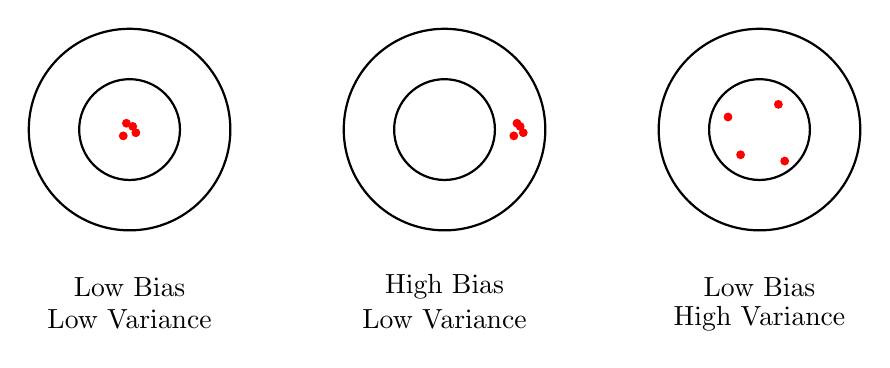
\begin{tikzpicture}[scale=0.8]
% Low bias, low variance
\begin{scope}[shift={(0,0)}]
\draw[thick] (0,0) circle (0.8);
\draw[thick] (0,0) circle (1.6);
\fill[red] (0.05,0.05) circle (2pt);
\fill[red] (-0.05,0.1) circle (2pt);
\fill[red] (0.1,-0.05) circle (2pt);
\fill[red] (-0.1,-0.1) circle (2pt);
\node at (0,-2.5) {Low Bias};
\node at (0,-3) {Low Variance};
\end{scope}

% High bias, low variance
\begin{scope}[shift={(5,0)}]
\draw[thick] (0,0) circle (0.8);
\draw[thick] (0,0) circle (1.6);
\fill[red] (1.2,0.05) circle (2pt);
\fill[red] (1.15,0.1) circle (2pt);
\fill[red] (1.25,-0.05) circle (2pt);
\fill[red] (1.1,-0.1) circle (2pt);
\node at (0,-2.5) {High Bias};
\node at (0,-3) {Low Variance};
\end{scope}

% Low bias, high variance
\begin{scope}[shift={(10,0)}]
\draw[thick] (0,0) circle (0.8);
\draw[thick] (0,0) circle (1.6);
\fill[red] (0.3,0.4) circle (2pt);
\fill[red] (-0.5,0.2) circle (2pt);
\fill[red] (0.4,-0.5) circle (2pt);
\fill[red] (-0.3,-0.4) circle (2pt);
\node at (0,-2.5) {Low Bias};
\node at (0,-3) {High Variance};
\end{scope}
\end{tikzpicture}
\caption{Bias-variance tradeoff visualization. Each dot represents a model trained on different data.}
\end{figure}

\subsection{Model Complexity and the Tradeoff}

\begin{keyidea}
As model complexity increases:
\begin{itemize}
\item \textbf{Bias decreases}: More flexible models can fit data better
\item \textbf{Variance increases}: More flexibility means more sensitivity to data
\end{itemize}

\textbf{Sweet spot}: Balance bias and variance to minimize total error.

\begin{figure}[H]
\centering
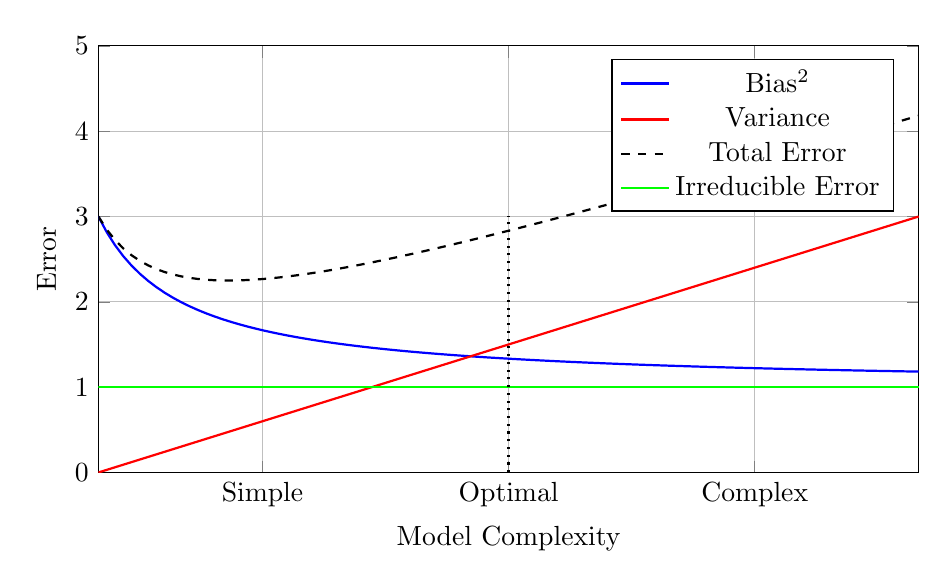
\begin{tikzpicture}
\begin{axis}[
    width=12cm,
    height=7cm,
    xlabel={Model Complexity},
    ylabel={Error},
    xmin=0, xmax=10,
    ymin=0, ymax=5,
    legend pos=north east,
    grid=major,
    xtick={2,5,8},
    xticklabels={Simple, Optimal, Complex}
]
\addplot[blue, thick, domain=0:10, samples=100] {2/(x+1) + 1};
\addlegendentry{Bias$^2$}

\addplot[red, thick, domain=0:10, samples=100] {0.3*x};
\addlegendentry{Variance}

\addplot[black, thick, dashed, domain=0:10, samples=100] {2/(x+1) + 0.3*x + 1};
\addlegendentry{Total Error}

\addplot[green, thick, domain=0:10, samples=100] {0*x + 1};
\addlegendentry{Irreducible Error}

\draw[dotted, thick] (axis cs:5,0) -- (axis cs:5,3);
\end{axis}
\end{tikzpicture}
\caption{Bias-variance tradeoff as a function of model complexity}
\end{figure}
\end{keyidea}

\subsection{Examples by Model Type}

\begin{table}[H]
\centering
\begin{tabular}{@{}lll@{}}
\toprule
Model & Bias & Variance \\
\midrule
Linear Regression & High (if data non-linear) & Low \\
High-degree Polynomial & Low & High \\
KNN with $k=1$ & Low & High \\
KNN with large $k$ & High & Low \\
Shallow Decision Tree & High & Low \\
Deep Decision Tree & Low & High \\
\bottomrule
\end{tabular}
\caption{Bias-variance characteristics of different models}
\end{table}

\subsection{Controlling the Tradeoff}

\subsubsection{Cross-Validation}

\begin{definition}[$k$-Fold Cross-Validation]
\begin{enumerate}
\item Split data into $k$ equal folds
\item For $i = 1, \ldots, k$:
\begin{itemize}
\item Train on folds $\{1, \ldots, k\} \setminus \{i\}$
\item Validate on fold $i$
\item Record error $E_i$
\end{itemize}
\item Report average: $\text{CV Error} = \frac{1}{k}\sum_{i=1}^k E_i$
\end{enumerate}

Common choice: $k = 5$ or $k = 10$.
\end{definition}

\textbf{Use}: Select hyperparameters (e.g., polynomial degree, regularization $\lambda$, tree depth) by choosing the value with lowest CV error.

\begin{definition}[Leave-One-Out Cross-Validation (LOOCV)]
Special case with $k = n$ (number of examples). Train on $n-1$ examples, test on 1. Repeat for each example.

\textbf{Pros}: Maximum training data, nearly unbiased estimate

\textbf{Cons}: Computationally expensive ($n$ model fits)
\end{definition}

\subsubsection{Regularization}

As discussed earlier, regularization (Ridge, Lasso, ElasticNet) explicitly controls model complexity:
\begin{itemize}
\item Increases bias (restricts model flexibility)
\item Decreases variance (less overfitting)
\item Tune $\lambda$ via cross-validation to find optimal tradeoff
\end{itemize}

\subsubsection{Ensemble Methods}

Preview of Part 3: Combining multiple models can reduce variance without increasing bias:
\begin{itemize}
\item \textbf{Bagging} (e.g., Random Forests): Reduces variance by averaging
\item \textbf{Boosting} (e.g., XGBoost): Reduces bias by sequential learning
\end{itemize}

\subsection{Summary of Part 1}

\begin{tcolorbox}[colback=yellow!10!white,colframe=orange!75!black,title=Key Takeaways]
\begin{enumerate}
\item \textbf{Linear Regression}: Foundation of supervised learning. Normal equation for closed-form; gradient descent for iterative solution.

\item \textbf{Regularization}: Ridge ($\ell_2$) for shrinkage, Lasso ($\ell_1$) for sparsity. Essential for high-dimensional data.

\item \textbf{Logistic Regression}: Linear model for classification using sigmoid function and cross-entropy loss.

\item \textbf{KNN}: Non-parametric, instance-based learning. Simple but suffers from curse of dimensionality.

\item \textbf{Decision Trees}: Interpretable, handles non-linear patterns. Prone to overfitting without pruning.

\item \textbf{Bias-Variance Tradeoff}: Fundamental tension in ML. Simple models: high bias, low variance. Complex models: low bias, high variance. Use cross-validation and regularization to balance.
\end{enumerate}

\textbf{Next Steps}: Part 2 explores probabilistic models (Naive Bayes, SVMs) that provide uncertainty estimates and maximum-margin classification.
\end{tcolorbox}

\begin{exercise}
\begin{enumerate}
\item Derive the gradient of Ridge regression loss and show it leads to $\vect{w}^* = (\mat{X}^\top\mat{X} + \lambda\mat{I})^{-1}\mat{X}^\top\vect{y}$.

\item Prove that the sigmoid derivative is $\sigma'(z) = \sigma(z)(1-\sigma(z))$.

\item For a dataset with 8 positive and 4 negative examples, compute the entropy. If a feature splits it into (6 pos, 1 neg) and (2 pos, 3 neg), compute the information gain.

\item Implement KNN ($k=3$) on 2D data: $\{(1,1,+), (2,2,+), (3,1,+), (6,5,-), (7,7,-), (8,6,-)\}$. Classify the point $(4,3)$.

\item For polynomial regression with degree $d$, how many parameters are in the model? How does this relate to overfitting as $d$ increases?

\item Draw a bias-variance diagram and mark where the following would fall: (a) $k=1$ KNN, (b) Linear regression on non-linear data, (c) Deep decision tree.
\end{enumerate}
\end{exercise}

% =======================
% Part 2: Probabilistic Models
% =======================
\addcontentsline{toc}{section}{Part 2: Probabilistic Models}
\section*{Part 2: Probabilistic Models}

\section{Naive Bayes}

\subsection{Probabilistic Classification Framework}

Unlike discriminative models (which learn $P(y|\vect{x})$ directly), \emph{generative models} learn the joint distribution $P(\vect{x}, y)$ and use Bayes' rule for prediction.

\begin{definition}[Bayes' Rule for Classification]
Given features $\vect{x}$ and class $y \in \{1, 2, \ldots, K\}$:
\[
P(y = c | \vect{x}) = \frac{P(\vect{x} | y = c) \cdot P(y = c)}{P(\vect{x})} = \frac{P(\vect{x} | y = c) \cdot P(y = c)}{\sum_{k=1}^K P(\vect{x} | y = k) \cdot P(y = k)}
\]
where:
\begin{itemize}
\item $P(y=c|\vect{x})$ is the \textbf{posterior} probability (what we want)
\item $P(\vect{x}|y=c)$ is the \textbf{likelihood} (how likely are these features given class $c$)
\item $P(y=c)$ is the \textbf{prior} (how common is class $c$ in general)
\item $P(\vect{x})$ is the \textbf{evidence} (normalization constant)
\end{itemize}
\end{definition}

\textbf{Classification rule}: 
\[
\hat{y} = \argmax_{c} P(y=c|\vect{x}) = \argmax_{c} P(\vect{x}|y=c) \cdot P(y=c)
\]
We can ignore $P(\vect{x})$ since it doesn't depend on $c$.

\subsection{The Naive Bayes Assumption}

\textbf{Challenge}: For $d$ features, estimating $P(\vect{x}|y=c) = P(x_1, x_2, \ldots, x_d | y=c)$ requires exponentially many parameters.

\textbf{Solution}: Assume \emph{conditional independence}.

\begin{definition}[Naive Bayes Assumption]
Features are conditionally independent given the class:
\[
P(\vect{x} | y = c) = P(x_1, x_2, \ldots, x_d | y = c) = \prod_{j=1}^d P(x_j | y = c)
\]
\end{definition}

\begin{intuition}
``Naive'' because we assume features don't interact given the class. For spam detection: knowing an email contains ``free'' doesn't change the probability of ``money'' appearing, given we know it's spam. This is often false in reality, but works surprisingly well in practice!
\end{intuition}

\begin{theorem}[Naive Bayes Classifier]
\[
\hat{y} = \argmax_{c} P(y=c) \prod_{j=1}^d P(x_j | y=c)
\]
In log space (for numerical stability):
\[
\hat{y} = \argmax_{c} \left[\log P(y=c) + \sum_{j=1}^d \log P(x_j | y=c)\right]
\]
\end{theorem}

\subsection{Estimating Parameters}

From training data $\mathcal{D} = \{(\vect{x}_i, y_i)\}_{i=1}^n$:

\begin{definition}[Prior Estimation]
\[
P(y = c) = \frac{\text{count}(y=c)}{n}
\]
Simply the fraction of training examples in class $c$.
\end{definition}

\begin{definition}[Likelihood Estimation]
Depends on the type of features:
\begin{itemize}
\item \textbf{Categorical}: $P(x_j = v | y=c) = \frac{\text{count}(x_j=v, y=c)}{\text{count}(y=c)}$
\item \textbf{Continuous}: Assume a distribution (e.g., Gaussian) and estimate parameters
\end{itemize}
\end{definition}

\subsection{Variants of Naive Bayes}

\subsubsection{Gaussian Naive Bayes}

For continuous features, assume each feature follows a Gaussian distribution.

\begin{definition}[Gaussian Naive Bayes]
Assume $P(x_j | y=c) \sim \mathcal{N}(\mu_{jc}, \sigma_{jc}^2)$:
\[
P(x_j | y=c) = \frac{1}{\sqrt{2\pi\sigma_{jc}^2}} \exp\left(-\frac{(x_j - \mu_{jc})^2}{2\sigma_{jc}^2}\right)
\]
where $\mu_{jc}$ and $\sigma_{jc}^2$ are estimated from training data:
\[
\mu_{jc} = \frac{1}{n_c}\sum_{i: y_i=c} x_{ij}, \quad \sigma_{jc}^2 = \frac{1}{n_c}\sum_{i: y_i=c} (x_{ij} - \mu_{jc})^2
\]
\end{definition}

\begin{example}[Medical Diagnosis]
Predict disease (yes/no) from symptoms: temperature and blood pressure.

\textbf{Training data}:
\begin{itemize}
\item Disease=Yes (3 examples): temps = [38.5, 39.0, 38.7], BP = [140, 145, 142]
\item Disease=No (2 examples): temps = [36.8, 37.1], BP = [120, 118]
\end{itemize}

\textbf{Estimates}:
\begin{itemize}
\item $P(\text{Disease}=\text{Yes}) = 3/5 = 0.6$
\item $\mu_{\text{temp,yes}} = 38.73$, $\sigma_{\text{temp,yes}}^2 = 0.043$
\item $\mu_{\text{temp,no}} = 36.95$, $\sigma_{\text{temp,no}}^2 = 0.0225$
\item Similar for blood pressure
\end{itemize}

\textbf{Test}: Patient with temp=38.0, BP=135. Compute both posteriors and predict the larger.
\end{example}

\subsubsection{Multinomial Naive Bayes}

For count data (e.g., word frequencies in documents).

\begin{definition}[Multinomial Naive Bayes]
Each feature $x_j$ is a count of how many times feature $j$ appears. Model:
\[
P(\vect{x} | y=c) = \frac{\left(\sum_j x_j\right)!}{\prod_j x_j!} \prod_{j=1}^d \theta_{jc}^{x_j}
\]
where $\theta_{jc} = P(\text{feature } j | y=c)$.

\textbf{Parameter estimation} (with Laplace smoothing):
\[
\theta_{jc} = \frac{\text{count}(x_j, y=c) + \alpha}{\sum_{j'} \text{count}(x_{j'}, y=c) + \alpha d}
\]
$\alpha > 0$ is a smoothing parameter (typically $\alpha=1$).
\end{definition}

\begin{intuition}
Laplace smoothing prevents zero probabilities. If a word never appears in spam training data, we still assign it a small non-zero probability rather than zero (which would make the entire product zero).
\end{intuition}

\begin{example}[Text Classification]
Classify documents as ``sports'' or ``politics''.

\textbf{Vocabulary}: \{game, team, vote, election, win\}

\textbf{Training}:
\begin{itemize}
\item Sports docs: ``game win'', ``team game'', ``team win win''
\item Politics docs: ``vote election'', ``election win''
\end{itemize}

\textbf{Word counts by class}:
\begin{itemize}
\item Sports: game=3, team=2, vote=0, election=0, win=4
\item Politics: game=0, team=0, vote=1, election=2, win=1
\end{itemize}

With $\alpha=1$:
\[
\theta_{\text{game,sports}} = \frac{3+1}{9+5} = \frac{4}{14} \approx 0.286
\]

\textbf{Test}: ``game election'' $\to$ compute $P(\text{sports}|\text{doc})$ and $P(\text{politics}|\text{doc})$.
\end{example}

\subsubsection{Bernoulli Naive Bayes}

For binary features (presence/absence).

\begin{definition}[Bernoulli Naive Bayes]
Each $x_j \in \{0, 1\}$ indicates feature presence:
\[
P(x_j | y=c) = \theta_{jc}^{x_j}(1-\theta_{jc})^{1-x_j}
\]
where $\theta_{jc} = P(x_j=1 | y=c)$.

\textbf{Estimation}:
\[
\theta_{jc} = \frac{\text{count}(x_j=1, y=c) + \alpha}{\text{count}(y=c) + 2\alpha}
\]
\end{definition}

\textbf{Multinomial vs Bernoulli}: Multinomial uses counts; Bernoulli uses only presence/absence. For text: Bernoulli asks ``Does word $j$ appear?''; Multinomial asks ``How many times?''

\subsection{Applications}

\begin{keyidea}
\textbf{Spam Filtering}:
\begin{itemize}
\item Features: words in email
\item Classes: spam / not spam
\item Use Multinomial or Bernoulli NB
\item Fast training and prediction
\end{itemize}

\textbf{Document Classification}:
\begin{itemize}
\item Categorize news articles, scientific papers
\item Large vocabularies: naive assumption helps reduce parameters
\end{itemize}

\textbf{Sentiment Analysis}:
\begin{itemize}
\item Classify reviews as positive/negative
\item Features: word frequencies or presence
\end{itemize}

\textbf{Advantages}:
\begin{itemize}
\item Simple, fast training and prediction
\item Works well with small training data
\item Handles high-dimensional data naturally
\item Probabilistic predictions (useful for uncertainty estimation)
\end{itemize}

\textbf{Limitations}:
\begin{itemize}
\item Strong independence assumption rarely holds
\item Poor at capturing feature interactions
\item Probability estimates can be extreme (overconfident)
\end{itemize}
\end{keyidea}

% =======================
\section{Generative vs Discriminative Models}
% =======================

\subsection{Key Distinction}

\begin{definition}[Discriminative Models]
Learn the conditional probability $P(y|\vect{x})$ directly.

\textbf{Examples}: Logistic regression, SVM, decision trees, neural networks

\textbf{Goal}: Find the decision boundary separating classes
\end{definition}

\begin{definition}[Generative Models]
Learn the joint probability $P(\vect{x}, y) = P(\vect{x}|y)P(y)$ and use Bayes' rule.

\textbf{Examples}: Naive Bayes, Gaussian Discriminant Analysis, HMMs

\textbf{Goal}: Model how data is generated for each class
\end{definition}

\begin{table}[H]
\centering
\begin{tabular}{@{}lll@{}}
\toprule
Aspect & Generative & Discriminative \\
\midrule
Learns & $P(\vect{x}, y)$ & $P(y|\vect{x})$ \\
Can sample new data? & Yes & No \\
Outlier detection & Natural & Difficult \\
Performance (large data) & Often worse & Often better \\
Performance (small data) & Often better & Often worse \\
Can handle missing features? & Yes (naturally) & Difficult \\
\bottomrule
\end{tabular}
\caption{Generative vs discriminative models}
\end{table}

\begin{intuition}
\textbf{Generative}: ``I understand what cats and dogs look like. Let me generate examples of each and see which your image resembles.''

\textbf{Discriminative}: ``I just need to distinguish cats from dogs. Let me find the boundary that separates them best.''

Generative models do more (model full distribution), so they need more assumptions. Discriminative models focus only on the decision boundary, often giving better classification.
\end{intuition}

\subsection{Gaussian Discriminant Analysis (GDA)}

GDA is a generative classifier that models each class as a multivariate Gaussian.

\begin{definition}[GDA Model]
For binary classification ($y \in \{0, 1\}$):
\begin{align}
y &\sim \text{Bernoulli}(\phi) \\
\vect{x}|y=0 &\sim \mathcal{N}(\vect{\mu}_0, \mat{\Sigma}) \\
\vect{x}|y=1 &\sim \mathcal{N}(\vect{\mu}_1, \mat{\Sigma})
\end{align}
Note: We assume the \emph{same} covariance $\mat{\Sigma}$ for both classes.
\end{definition}

\begin{theorem}[GDA Parameters]
Maximum likelihood estimates from data $\{(\vect{x}_i, y_i)\}_{i=1}^n$:
\begin{align}
\phi &= \frac{1}{n} \sum_{i=1}^n \mathbb{I}(y_i = 1), \\
\boldsymbol{\mu}_0 &= \frac{\sum_{i=1}^n \mathbb{I}(y_i = 0)\,\boldsymbol{x}_i}{\sum_{i=1}^n \mathbb{I}(y_i = 0)}, \\
\boldsymbol{\mu}_1 &= \frac{\sum_{i=1}^n \mathbb{I}(y_i = 1)\,\boldsymbol{x}_i}{\sum_{i=1}^n \mathbb{I}(y_i = 1)}, \\
\boldsymbol{\Sigma} &= \frac{1}{n} \sum_{i=1}^n \bigl(\boldsymbol{x}_i - \boldsymbol{\mu}_{y_i}\bigr)\bigl(\boldsymbol{x}_i - \boldsymbol{\mu}_{y_i}\bigr)^\top.
\end{align}
\end{theorem}

\begin{theorem}[GDA Decision Boundary]
The decision boundary where $P(y=1|\vect{x}) = P(y=0|\vect{x})$ is linear:
\[
\vect{w}^\top\vect{x} + w_0 = 0
\]
where $\vect{w} = \mat{\Sigma}^{-1}(\vect{\mu}_1 - \vect{\mu}_0)$ and $w_0$ involves $\phi$, $\vect{\mu}_0$, $\vect{\mu}_1$.

This shows GDA produces a linear classifier, similar to logistic regression!
\end{theorem}

\begin{keyidea}
\textbf{GDA vs Logistic Regression}:
\begin{itemize}
\item Both produce linear decision boundaries
\item GDA makes stronger assumptions (Gaussian distributions)
\item If assumptions hold, GDA is more efficient (needs less data)
\item If assumptions violated, logistic regression is more robust
\item GDA can be viewed as a special case that implies logistic regression
\end{itemize}

\textbf{Rule of thumb}: Try both. If data looks roughly Gaussian, GDA may work better. Otherwise, prefer logistic regression.
\end{keyidea}

\subsection{Hidden Markov Models (Brief Overview)}

\begin{definition}[Hidden Markov Model (HMM)]
A sequence model with:
\begin{itemize}
\item \textbf{Hidden states} $z_1, z_2, \ldots, z_T$ (not observed)
\item \textbf{Observations} $x_1, x_2, \ldots, x_T$ (observed)
\item \textbf{Transition probabilities}: $P(z_t | z_{t-1})$
\item \textbf{Emission probabilities}: $P(x_t | z_t)$
\end{itemize}
\end{definition}

\begin{intuition}
Think of speech recognition: hidden states are phonemes (sound units), observations are audio features. We observe the audio but want to infer the underlying phoneme sequence.
\end{intuition}

\textbf{Key algorithms}:
\begin{itemize}
\item \textbf{Forward-Backward}: Compute $P(\vect{x})$ (likelihood)
\item \textbf{Viterbi}: Find most likely hidden state sequence $\argmax_{\vect{z}} P(\vect{z}|\vect{x})$
\item \textbf{Baum-Welch}: Learn parameters (EM algorithm)
\end{itemize}

\textbf{Applications}: Speech recognition, part-of-speech tagging, bioinformatics (gene prediction).

\begin{remark}
HMMs are beyond the scope of this introductory treatment. They represent an important class of generative models for sequential data. Modern alternatives include RNNs and Transformers (covered in Part 4).
\end{remark}

% =======================
\section{Support Vector Machines}
% =======================

\subsection{Intuition: Maximum Margin Classification}

Unlike logistic regression (which finds \emph{any} separating hyperplane), SVM finds the hyperplane with the \emph{largest margin}.

\begin{definition}[Margin]
The \emph{margin} is the distance from the decision boundary to the nearest data point.

A \emph{maximum margin classifier} maximizes this distance.
\end{definition}

\begin{intuition}
Imagine two classes of points that are linearly separable. Many hyperplanes separate them, but intuitively, the one in the ``middle'' (farthest from both classes) is most robust to noise and generalizes better.
\end{intuition}

\begin{figure}[H]
\centering
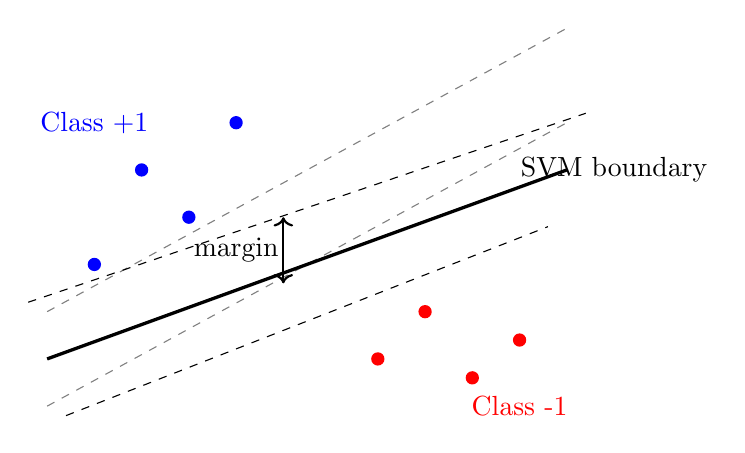
\begin{tikzpicture}[scale=1.2]
% Data points
\foreach \point in {(1,2), (1.5,3), (2,2.5), (2.5,3.5)}
    \fill[blue] \point circle (2pt);
\foreach \point in {(4,1), (4.5,1.5), (5,0.8), (5.5,1.2)}
    \fill[red] \point circle (2pt);

% Three possible separators
\draw[gray, dashed] (0.5,0.5) -- (6,3.5);
\draw[gray, dashed] (0.5,1.5) -- (6,4.5);
\draw[black, very thick] (0.5,1) -- (6,3);

% Margin lines
\draw[black, dashed] (0.7,0.4) -- (5.8,2.4);
\draw[black, dashed] (0.3,1.6) -- (6.2,3.6);

% Annotations
\draw[<->, thick] (3,1.8) -- (3,2.5);
\node at (2.5,2.15) {margin};
\node[blue] at (1,3.5) {Class +1};
\node[red] at (5.5,0.5) {Class -1};
\node at (6.5,3) {SVM boundary};
\end{tikzpicture}
\caption{SVM finds the hyperplane with maximum margin (thick line) between classes}
\end{figure}

\subsection{Mathematical Formulation (Hard Margin)}

\begin{definition}[Linear Classifier]
Decision function: $f(\vect{x}) = \vect{w}^\top\vect{x} + b$

Prediction: $\hat{y} = \text{sign}(f(\vect{x})) = \begin{cases} +1 & \text{if } f(\vect{x}) > 0 \\ -1 & \text{if } f(\vect{x}) < 0 \end{cases}$
\end{definition}

\begin{definition}[Functional and Geometric Margin]
\textbf{Functional margin} of $(\vect{w}, b)$ with respect to $(\vect{x}_i, y_i)$:
\[
\hat{\gamma}_i = y_i(\vect{w}^\top\vect{x}_i + b)
\]
Positive when correctly classified.

\textbf{Geometric margin} (actual distance to hyperplane):
\[
\gamma_i = \frac{y_i(\vect{w}^\top\vect{x}_i + b)}{\norm{\vect{w}}}
\]
\end{definition}

\begin{theorem}[Hard Margin SVM (Primal Form)]
To maximize the margin:
\[
\begin{aligned}
\max_{\vect{w}, b} \quad & \frac{1}{\norm{\vect{w}}} \\
\text{subject to} \quad & y_i(\vect{w}^\top\vect{x}_i + b) \geq 1, \quad i = 1, \ldots, n
\end{aligned}
\]
Equivalently (minimization form):
\[
\begin{aligned}
\min_{\vect{w}, b} \quad & \frac{1}{2}\norm{\vect{w}}^2 \\
\text{subject to} \quad & y_i(\vect{w}^\top\vect{x}_i + b) \geq 1, \quad i = 1, \ldots, n
\end{aligned}
\]
\end{theorem}

\begin{intuition}
The constraint $y_i(\vect{w}^\top\vect{x}_i + b) \geq 1$ ensures all points are correctly classified and at least distance $1/\norm{\vect{w}}$ from the boundary. Minimizing $\norm{\vect{w}}^2$ maximizes the margin $1/\norm{\vect{w}}$.
\end{intuition}

\subsection{Lagrange Duality and the Dual Form}

The primal is a constrained optimization problem. We use Lagrange multipliers.

\begin{definition}[Lagrangian]
\[
\mathcal{L}(\vect{w}, b, \vect{\alpha}) = \frac{1}{2}\norm{\vect{w}}^2 - \sum_{i=1}^n \alpha_i[y_i(\vect{w}^\top\vect{x}_i + b) - 1]
\]
where $\alpha_i \geq 0$ are Lagrange multipliers.
\end{definition}

\begin{theorem}[KKT Conditions]
At the optimum:
\begin{enumerate}
\item $\nabla_{\vect{w}} \mathcal{L} = 0 \implies \vect{w} = \sum_{i=1}^n \alpha_i y_i \vect{x}_i$
\item $\pp{\mathcal{L}}{b} = 0 \implies \sum_{i=1}^n \alpha_i y_i = 0$
\item $\alpha_i \geq 0$
\item $\alpha_i [y_i(\vect{w}^\top\vect{x}_i + b) - 1] = 0$ (complementary slackness)
\end{enumerate}
\end{theorem}

\begin{keyidea}
The complementary slackness condition is crucial:
\begin{itemize}
\item If $\alpha_i > 0$, then $y_i(\vect{w}^\top\vect{x}_i + b) = 1$ (point is on the margin)
\item These points are called \textbf{support vectors}
\item Only support vectors affect the decision boundary!
\item Most $\alpha_i = 0$ $\to$ sparse solution
\end{itemize}
\end{keyidea}

\begin{theorem}[Dual Form]
Substituting the KKT conditions into the Lagrangian:
\[
\begin{aligned}
\max_{\vect{\alpha}} \quad & \sum_{i=1}^n \alpha_i - \frac{1}{2}\sum_{i=1}^n\sum_{j=1}^n \alpha_i\alpha_j y_i y_j \vect{x}_i^\top\vect{x}_j \\
\text{subject to} \quad & \alpha_i \geq 0, \quad i = 1, \ldots, n \\
& \sum_{i=1}^n \alpha_i y_i = 0
\end{aligned}
\]
This is a \emph{quadratic programming} problem in $\vect{\alpha}$.
\end{theorem}

\textbf{Why dual is useful}:
\begin{itemize}
\item Only depends on dot products $\vect{x}_i^\top\vect{x}_j$ (enables kernel trick!)
\item Sparse solution (most $\alpha_i = 0$)
\item Once solved, prediction: $f(\vect{x}) = \sum_{i=1}^n \alpha_i y_i \vect{x}_i^\top\vect{x} + b$
\end{itemize}

\subsection{The Kernel Trick}

\textbf{Problem}: What if data is not linearly separable?

\textbf{Solution}: Map data to higher-dimensional space where it becomes separable!

\begin{definition}[Feature Map]
Let $\vect{\phi}: \R^d \to \R^D$ (with $D \gg d$) be a feature map.

Transform: $\vect{x} \to \vect{\phi}(\vect{x})$

Run SVM in the transformed space: $f(\vect{x}) = \vect{w}^\top\vect{\phi}(\vect{x}) + b$
\end{definition}

\begin{example}[Simple Kernel]
For $\vect{x} = [x_1, x_2]^\top$, define:
\[
\vect{\phi}(\vect{x}) = [x_1^2, \sqrt{2}x_1x_2, x_2^2, \sqrt{2}x_1, \sqrt{2}x_2, 1]^\top
\]
This maps 2D to 6D. Data that's not linearly separable in 2D might be in 6D!
\end{example}

\textbf{Issue}: Computing $\vect{\phi}(\vect{x})$ explicitly for high $D$ is expensive.

\begin{theorem}[Kernel Trick]
We only need dot products $\vect{\phi}(\vect{x}_i)^\top\vect{\phi}(\vect{x}_j)$ in the dual.

Define \textbf{kernel function}: $K(\vect{x}_i, \vect{x}_j) = \vect{\phi}(\vect{x}_i)^\top\vect{\phi}(\vect{x}_j)$

If we can compute $K$ directly without computing $\vect{\phi}$ explicitly, we get efficiency!
\end{theorem}

\begin{definition}[Common Kernels]
\begin{itemize}
\item \textbf{Linear}: $K(\vect{x}, \vect{z}) = \vect{x}^\top\vect{z}$

\item \textbf{Polynomial}: $K(\vect{x}, \vect{z}) = (\vect{x}^\top\vect{z} + c)^p$

Corresponds to all polynomials up to degree $p$.

\item \textbf{RBF (Radial Basis Function / Gaussian)}: 
\[
K(\vect{x}, \vect{z}) = \exp\left(-\gamma\norm{\vect{x} - \vect{z}}^2\right)
\]
where $\gamma > 0$ is a bandwidth parameter.

This corresponds to \emph{infinite-dimensional} feature space!

\item \textbf{Sigmoid}: $K(\vect{x}, \vect{z}) = \tanh(\alpha \vect{x}^\top\vect{z} + c)$
\end{itemize}
\end{definition}

\begin{keyidea}
\textbf{The kernel trick magic}:

The polynomial kernel $(x^\top z + 1)^2$ computes the dot product in a space of all degree-2 polynomials:
\[
(x^\top z + 1)^2 = (x_1z_1 + x_2z_2 + 1)^2 = x_1^2z_1^2 + 2x_1x_2z_1z_2 + x_2^2z_2^2 + 2x_1z_1 + 2x_2z_2 + 1
\]
This equals $\vect{\phi}(\vect{x})^\top\vect{\phi}(\vect{z})$ with $\vect{\phi}(\vect{x}) = [x_1^2, \sqrt{2}x_1x_2, x_2^2, \sqrt{2}x_1, \sqrt{2}x_2, 1]^\top$.

We computed this in $O(d)$ time instead of $O(D)$ where $D=\binom{d+2}{2}$!

For RBF kernel: we operate in infinite dimensions without ever computing infinite-dimensional vectors!
\end{keyidea}

\begin{theorem}[Kernelized Dual]
With kernel $K$:
\[
\begin{aligned}
\max_{\vect{\alpha}} \quad & \sum_{i=1}^n \alpha_i - \frac{1}{2}\sum_{i=1}^n\sum_{j=1}^n \alpha_i\alpha_j y_i y_j K(\vect{x}_i, \vect{x}_j) \\
\text{subject to} \quad & \alpha_i \geq 0, \sum_{i=1}^n \alpha_i y_i = 0
\end{aligned}
\]
Prediction: $f(\vect{x}) = \sum_{i=1}^n \alpha_i y_i K(\vect{x}_i, \vect{x}) + b$
\end{theorem}

\subsection{Soft Margin SVM}

\textbf{Problem}: Real data is rarely perfectly separable. Hard margin SVM fails if any point violates the constraint.

\textbf{Solution}: Allow some misclassifications with penalty.

\begin{definition}[Slack Variables]
Introduce $\xi_i \geq 0$ for each point:
\begin{itemize}
\item $\xi_i = 0$: Point correctly classified with margin $\geq 1$
\item $0 < \xi_i < 1$: Correctly classified but within margin
\item $\xi_i \geq 1$: Misclassified
\end{itemize}
Relaxed constraint: $y_i(\vect{w}^\top\vect{x}_i + b) \geq 1 - \xi_i$
\end{definition}

\begin{theorem}[Soft Margin SVM]
\[
\begin{aligned}
\min_{\vect{w}, b, \vect{\xi}} \quad & \frac{1}{2}\norm{\vect{w}}^2 + C\sum_{i=1}^n \xi_i \\
\text{subject to} \quad & y_i(\vect{w}^\top\vect{x}_i + b) \geq 1 - \xi_i \\
& \xi_i \geq 0, \quad i = 1, \ldots, n
\end{aligned}
\]
$C > 0$ is a hyperparameter controlling the trade-off:
\begin{itemize}
\item Large $C$: Fewer violations allowed (closer to hard margin, may overfit)
\item Small $C$: More violations allowed (more regularization, may underfit)
\end{itemize}
\end{theorem}

\begin{intuition}
Soft margin balances two goals:
\begin{enumerate}
\item Maximize margin (minimize $\norm{\vect{w}}^2$)
\item Minimize classification errors (minimize $\sum \xi_i$)
\end{enumerate}
Parameter $C$ controls this trade-off. Use cross-validation to choose $C$.
\end{intuition}

\begin{definition}[Hinge Loss Formulation]
Soft margin SVM can be written as:
\[
\min_{\vect{w}, b} \frac{1}{2}\norm{\vect{w}}^2 + C\sum_{i=1}^n \max(0, 1 - y_i(\vect{w}^\top\vect{x}_i + b))
\]
where $\ell_{\text{hinge}}(z) = \max(0, 1-z)$ is the hinge loss.

This connects SVM to other loss functions (logistic loss, squared loss, etc.).
\end{definition}

\subsection{Support Vector Regression (SVR)}

SVM can also be used for regression!

\begin{definition}[$\epsilon$-insensitive Loss]
\[
\ell_\epsilon(y, \hat{y}) = \begin{cases}
0 & \text{if } |y - \hat{y}| < \epsilon \\
|y - \hat{y}| - \epsilon & \text{otherwise}
\end{cases}
\]
No penalty for predictions within $\epsilon$ of the true value.
\end{definition}

\begin{definition}[SVR Formulation]
\[
\begin{aligned}
\min_{\vect{w}, b} \quad & \frac{1}{2}\norm{\vect{w}}^2 + C\sum_{i=1}^n (\xi_i + \xi_i^*)\\
\text{subject to} \quad & y_i - (\vect{w}^\top\vect{x}_i + b) \leq \epsilon + \xi_i \\
& (\vect{w}^\top\vect{x}_i + b) - y_i \leq \epsilon + \xi_i^* \\
& \xi_i, \xi_i^* \geq 0
\end{aligned}
\]
\end{definition}

\begin{intuition}
SVR fits a ``tube'' of width $2\epsilon$ around the data. Points inside the tube have no penalty. Points outside pay a linear penalty proportional to their distance from the tube.
\end{intuition}

\subsection{Practical Considerations}

\begin{implementationbox}
\textbf{Choosing SVM Parameters}:

\begin{itemize}
\item \textbf{Kernel}: Start with RBF (most flexible). Try linear if $d$ is large.
\item \textbf{$C$}: Controls regularization. Use grid search + CV.
\item \textbf{$\gamma$ (for RBF)}: Controls kernel width. Small $\gamma$ = wide kernel (smooth), large $\gamma$ = narrow kernel (complex boundary).
\end{itemize}

\textbf{Feature Scaling}: Critical for SVMs! Since they use distances, features should be normalized (e.g., to $[0,1]$ or standardized to mean 0, std 1).

\textbf{Complexity}:
\begin{itemize}
\item Training: $O(n^2 d)$ to $O(n^3)$ (solving QP)
\item Prediction: $O(n_{\text{sv}} d)$ where $n_{\text{sv}}$ is number of support vectors
\end{itemize}

\textbf{When to use SVMs}:
\begin{itemize}
\item Medium-sized datasets (1000s to 100,000s of examples)
\item High-dimensional data (works well when $d > n$)
\item When you need a strong theoretical guarantee (maximum margin)
\item Non-linear decision boundaries (with kernels)
\end{itemize}

\textbf{When NOT to use SVMs}:
\begin{itemize}
\item Very large datasets ($n > 1$M) - use linear models or neural networks
\item When interpretability is critical - use decision trees or linear models
\item When probabilistic outputs are essential - use logistic regression or Naive Bayes
\end{itemize}
\end{implementationbox}

\subsection{Summary of Part 2}

\begin{tcolorbox}[colback=yellow!10!white,colframe=orange!75!black,title=Key Takeaways]
\begin{enumerate}
\item \textbf{Naive Bayes}: Generative classifier using Bayes' rule with conditional independence assumption. Fast, works well for text classification despite ``naive'' assumption.

\item \textbf{Generative vs Discriminative}: Generative models ($P(\vect{x}, y)$) model how data is generated; discriminative models ($P(y|\vect{x})$) focus on decision boundaries. Trade-offs in performance, data requirements, and capabilities.

\item \textbf{GDA}: Assumes Gaussian distributions per class. Produces linear boundaries like logistic regression but with stronger assumptions.

\item \textbf{SVM}: Maximum margin classifier. Primal form maximizes margin; dual form enables kernel trick. Soft margin allows violations with penalty $C$.

\item \textbf{Kernel Trick}: Implicitly maps to high (or infinite) dimensional spaces via kernel functions. RBF kernel most popular for non-linear boundaries.

\item \textbf{SVR}: Adapts SVM for regression using $\epsilon$-insensitive loss. Fits tube around data.
\end{enumerate}

\textbf{Next Steps}: Part 3 explores ensemble methods (Bagging, Boosting, Stacking) that combine multiple models to achieve better performance than any single model.
\end{tcolorbox}

\begin{exercise}
\begin{enumerate}
\item Given training data for spam (words: ``free''=10, ``money''=8) and ham (``free''=2, ``money''=1), with priors $P(\text{spam})=0.4$, compute $P(\text{spam}|\text{``free money''})$ using Multinomial Naive Bayes with Laplace smoothing ($\alpha=1$).

\item Prove that if we assume Gaussian distributions with same covariance for both classes (GDA), the posterior $P(y=1|\vect{x})$ has the form of logistic regression.

\item For the polynomial kernel $K(\vect{x}, \vect{z}) = (\vect{x}^\top\vect{z} + 1)^2$, explicitly write out the feature map $\vect{\phi}(\vect{x})$ for $\vect{x} \in \R^2$.

\item Show that the RBF kernel $K(\vect{x}, \vect{z}) = \exp(-\gamma\norm{\vect{x}-\vect{z}}^2)$ satisfies the property $K(\vect{x}, \vect{x}) = 1$ and $K(\vect{x}, \vect{z}) \to 0$ as $\norm{\vect{x}-\vect{z}} \to \infty$.

\item Consider a 1D SVM with data $\{(1, +1), (2, +1), (4, -1), (5, -1)\}$. Assuming hard margin is feasible, what are the support vectors?

\item Explain why feature scaling is critical for SVMs but not for decision trees.
\end{enumerate}
\end{exercise}

% =======================
% Part 3: Ensemble Methods
% =======================
\addcontentsline{toc}{section}{Part 3: Ensemble Methods}
\section*{Part 3: Ensemble Methods}

\section{Introduction to Ensemble Learning}

\begin{definition}[Ensemble Learning]
An \emph{ensemble method} combines predictions from multiple base models (called \emph{learners} or \emph{weak learners}) to produce a final prediction that is typically more accurate and robust than any individual model.
\end{definition}

\begin{intuition}
``Wisdom of crowds'': Just as a group of people can make better decisions than individuals, combining multiple models can reduce errors. Different models make different mistakes; by aggregating, we can cancel out individual errors.
\end{intuition}

\begin{keyidea}
\textbf{Why Ensembles Work}:

From the bias-variance perspective:
\begin{itemize}
\item \textbf{Reduce Variance}: Average multiple high-variance models (e.g., deep trees) $\to$ more stable predictions
\item \textbf{Reduce Bias}: Sequentially build models that correct errors of previous ones $\to$ better fit
\item \textbf{Improve Robustness}: Different models capture different patterns; ensemble is less likely to fail
\end{itemize}

\textbf{Three Main Paradigms}:
\begin{enumerate}
\item \textbf{Bagging}: Train models independently on bootstrap samples, then average (reduces variance)
\item \textbf{Boosting}: Train models sequentially, each focusing on previous errors (reduces bias)
\item \textbf{Stacking}: Train a meta-model to combine base model predictions (learns optimal combination)
\end{enumerate}
\end{keyidea}

% =======================
\section{Bagging (Bootstrap Aggregating)}
% =======================

\subsection{Bootstrap Sampling}

\begin{definition}[Bootstrap Sample]
Given a dataset $\mathcal{D}$ of size $n$, a \emph{bootstrap sample} $\mathcal{D}_i$ is created by:
\begin{enumerate}
\item Randomly sample $n$ examples from $\mathcal{D}$ \emph{with replacement}
\item Some examples appear multiple times, others not at all
\end{enumerate}

On average, about 63.2\% of unique examples appear in each bootstrap sample.
\end{definition}

\begin{proof}[Why 63.2\%?]
Probability that example $i$ is NOT selected in one draw: $(1 - 1/n)$

Probability NOT selected in $n$ draws: $(1 - 1/n)^n$

As $n \to \infty$: $(1 - 1/n)^n \to e^{-1} \approx 0.368$

So probability of being selected: $1 - 0.368 = 0.632$ or 63.2\%.
\end{proof}

\subsection{Bagging Algorithm}

\begin{algorithmbox}
\textbf{Bagging for Classification/Regression}

\textbf{Input}: 
\begin{itemize}
\item Training data $\mathcal{D} = \{(\vect{x}_i, y_i)\}_{i=1}^n$
\item Base learning algorithm $\mathcal{A}$
\item Number of models $M$
\end{itemize}

\textbf{Training}:
\begin{enumerate}
\item \textbf{For} $m = 1$ to $M$:
\begin{itemize}
\item Create bootstrap sample $\mathcal{D}_m$ by sampling $n$ examples from $\mathcal{D}$ with replacement
\item Train base learner: $h_m = \mathcal{A}(\mathcal{D}_m)$
\end{itemize}
\end{enumerate}

\textbf{Prediction} for new example $\vect{x}$:
\begin{itemize}
\item \textbf{Classification}: $\hat{y} = \text{majority\_vote}(h_1(\vect{x}), h_2(\vect{x}), \ldots, h_M(\vect{x}))$
\item \textbf{Regression}: $\hat{y} = \frac{1}{M}\sum_{m=1}^M h_m(\vect{x})$
\end{itemize}

\textbf{Output}: Ensemble predictor $H(\vect{x})$
\end{algorithmbox}

\begin{theorem}[Variance Reduction in Bagging]
Suppose we have $M$ independent models, each with variance $\sigma^2$ and we average their predictions. The variance of the ensemble is:
\[
\Var(\text{average}) = \frac{\sigma^2}{M}
\]
If models are correlated with correlation $\rho$:
\[
\Var(\text{average}) = \rho\sigma^2 + \frac{1-\rho}{M}\sigma^2
\]
As $M \to \infty$, variance approaches $\rho\sigma^2$.
\end{theorem}

\begin{keyidea}
Bagging reduces variance most when:
\begin{enumerate}
\item Base learners have high variance (e.g., deep decision trees)
\item Base learners are diverse (low correlation $\rho$)
\end{enumerate}

This is why bagging works best with unstable algorithms like decision trees, but doesn't help much with stable algorithms like linear regression.
\end{keyidea}

\subsection{Random Forests}

Random Forests extend bagging by adding another source of randomness.

\begin{definition}[Random Forest]
A Random Forest is an ensemble of decision trees where:
\begin{enumerate}
\item Each tree is trained on a bootstrap sample (like bagging)
\item \textbf{Additional randomness}: At each split, only a random subset of $m$ features is considered (out of total $d$ features)
\end{enumerate}
\end{definition}

\textbf{Feature subset size $m$}:
\begin{itemize}
\item Classification: $m = \lfloor\sqrt{d}\rfloor$ (default)
\item Regression: $m = \lfloor d/3 \rfloor$ (default)
\item Can tune via cross-validation
\end{itemize}

\begin{intuition}
Why limit features at each split?

Without this, trees in bagging would be similar---they'd all split on the strongest features first. By randomly limiting choices, we force trees to consider different features, increasing diversity and decorrelating predictions.
\end{intuition}

\begin{algorithmbox}
\textbf{Random Forest Algorithm}

\textbf{Input}: Data $\mathcal{D}$, number of trees $M$, feature subset size $m$

\textbf{For} $i = 1$ to $M$:
\begin{enumerate}
\item Draw bootstrap sample $\mathcal{D}_i$ from $\mathcal{D}$
\item Grow tree $T_i$ on $\mathcal{D}_i$:
\begin{itemize}
\item At each node, randomly select $m$ features from $d$ total
\item Choose best split among these $m$ features only
\item Split and recurse until stopping criterion
\item Do NOT prune trees (grow to maximum depth or min samples)
\end{itemize}
\end{enumerate}

\textbf{Prediction}: Average (regression) or vote (classification) across all $M$ trees.
\end{algorithmbox}

\begin{figure}
    \centering
    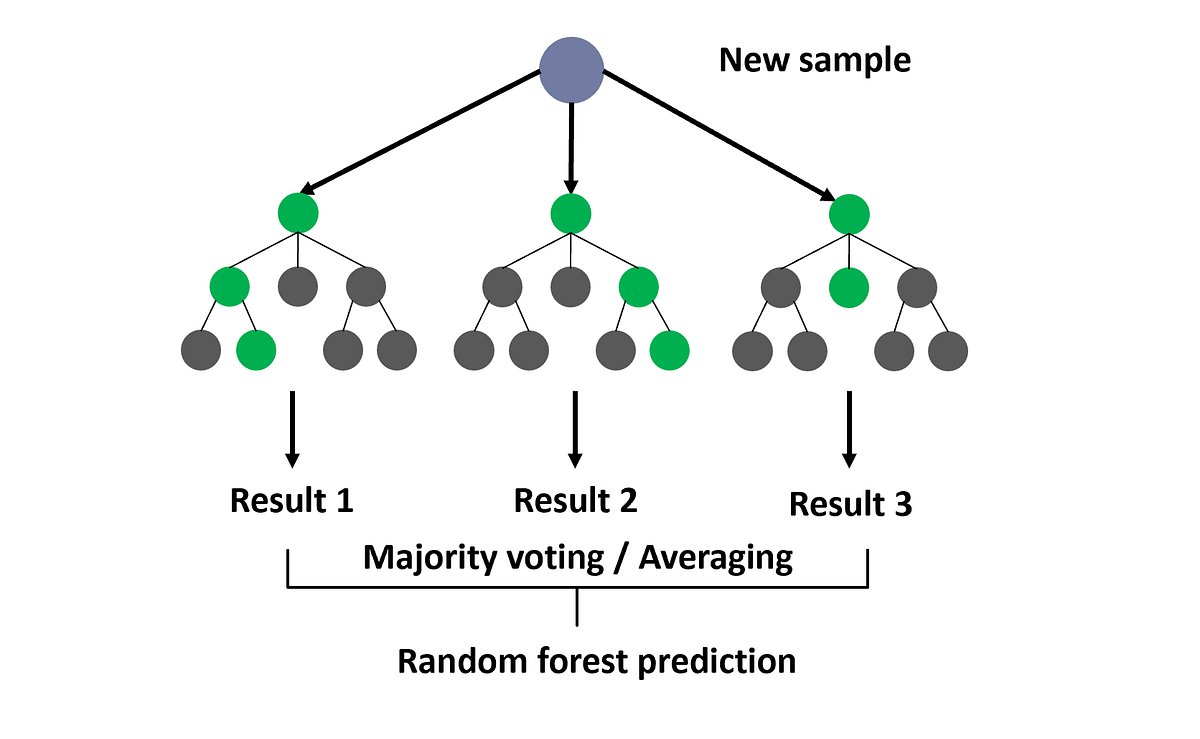
\includegraphics[width=1\linewidth]{Random_Forest.png}
    \caption{Random Forest: Multiple diverse trees vote for final prediction}
    \label{fig:randomforest}
\end{figure}

\subsection{Out-of-Bag (OOB) Error Estimation}

\begin{definition}[Out-of-Bag (OOB) Examples]
For each bootstrap sample, approximately 37\% of examples are \emph{not} selected. These are called \emph{out-of-bag} (OOB) examples for that tree.

For each data point $(\vect{x}_i, y_i)$, consider only trees where $i$ was OOB. Average their predictions to get OOB prediction for $\vect{x}_i$.
\end{definition}

\begin{definition}[OOB Error]
\[
\text{OOB Error} = \frac{1}{n}\sum_{i=1}^n \ell(y_i, \hat{y}_i^{\text{OOB}})
\]
where $\hat{y}_i^{\text{OOB}}$ is the prediction using only trees where $i$ was OOB.
\end{definition}

\begin{keyidea}
OOB error provides a free validation estimate!
\begin{itemize}
\item No need for separate validation set
\item Each example has been tested on $\approx 37\%$ of trees
\item Approximates cross-validation error
\item Can use to tune hyperparameters (number of trees, max depth, etc.)
\end{itemize}

This is a major practical advantage of Random Forests.
\end{keyidea}

\subsection{Feature Importance in Random Forests}

\begin{definition}[Mean Decrease in Impurity (MDI)]
For each feature $j$, compute the total reduction in impurity (Gini or entropy) when splitting on feature $j$, averaged over all trees and all nodes.

Higher values indicate more important features.
\end{definition}

\begin{definition}[Permutation Importance]
\begin{enumerate}
\item Compute baseline OOB error
\item For each feature $j$:
\begin{itemize}
\item Randomly permute feature $j$ in OOB data
\item Compute new OOB error
\item Importance = increase in error
\end{itemize}
\end{enumerate}

If permuting a feature greatly increases error, that feature is important.
\end{definition}

\subsection{Advantages and Limitations}

\begin{keyidea}
\textbf{Advantages of Random Forests}:
\begin{itemize}
\item \textbf{Excellent performance}: Often among the best off-the-shelf algorithms
\item \textbf{Minimal tuning}: Works well with default parameters
\item \textbf{Robust to overfitting}: Even with many trees
\item \textbf{Handles mixed data}: Numerical and categorical features
\item \textbf{Feature importance}: Built-in importance measures
\item \textbf{Parallelizable}: Trees trained independently
\item \textbf{OOB error}: Free validation estimate
\end{itemize}

\textbf{Limitations}:
\begin{itemize}
\item \textbf{Less interpretable}: Cannot visualize like a single tree
\item \textbf{Memory intensive}: Must store $M$ trees
\item \textbf{Slow prediction}: Must query $M$ trees
\item \textbf{Extrapolation}: Cannot predict beyond training range (averaging effect)
\item \textbf{Biased toward categorical features}: With many levels
\end{itemize}

\textbf{Typical hyperparameters}:
\begin{itemize}
\item Number of trees $M$: 100-1000 (more is usually better, diminishing returns)
\item Max features $m$: $\sqrt{d}$ for classification, $d/3$ for regression
\item Min samples per leaf: 1-10 (larger = more regularization)
\item Max depth: Usually unlimited (full trees)
\end{itemize}
\end{keyidea}

% =======================
\section{Boosting}
% =======================

\subsection{Boosting Philosophy}

Unlike bagging (parallel training), boosting trains models \emph{sequentially}, with each new model focusing on examples that previous models got wrong.

\begin{intuition}
Think of boosting as learning from mistakes:
\begin{enumerate}
\item Train model 1 on data
\item Identify examples model 1 struggles with
\item Train model 2 to focus on those hard examples
\item Combine models 1 and 2
\item Repeat, always focusing on current ensemble's weaknesses
\end{enumerate}

This reduces \emph{bias} by creating increasingly complex models that fit the data better.
\end{intuition}

\subsection{AdaBoost (Adaptive Boosting)}

AdaBoost adjusts weights on training examples, increasing weights on misclassified examples.

\begin{algorithmbox}
\textbf{AdaBoost for Binary Classification}

\textbf{Input}: Data $\{(\vect{x}_i, y_i)\}_{i=1}^n$ with $y_i \in \{-1, +1\}$, number of rounds $T$

\textbf{Initialize}: Weights $w_i^{(1)} = 1/n$ for all $i$

\textbf{For} $t = 1$ to $T$:
\begin{enumerate}
\item Train weak classifier $h_t$ on weighted data (minimizing weighted error):
\[
\epsilon_t = \sum_{i=1}^n w_i^{(t)} \,\mathbb{I}\bigl(h_t(\boldsymbol{x}_i) \neq y_i\bigr)
\]
\item Compute classifier weight:
\[
\alpha_t = \frac{1}{2}\ln\left(\frac{1-\epsilon_t}{\epsilon_t}\right)
\]
Higher $\alpha_t$ for more accurate classifiers.

\item Update example weights:
\[
w_i^{(t+1)} = w_i^{(t)} \cdot \exp(-\alpha_t y_i h_t(\vect{x}_i))
\]
\begin{itemize}
\item If correct ($y_i = h_t(\vect{x}_i)$): weight decreases
\item If incorrect ($y_i \neq h_t(\vect{x}_i)$): weight increases
\end{itemize}

\item Normalize: $w_i^{(t+1)} = w_i^{(t+1)} / \sum_j w_j^{(t+1)}$
\end{enumerate}

\textbf{Final classifier}:
\[
H(\vect{x}) = \text{sign}\left(\sum_{t=1}^T \alpha_t h_t(\vect{x})\right)
\]
\end{algorithmbox}

\begin{example}[AdaBoost Iteration]
Suppose after round 1:
\begin{itemize}
\item Examples 1,2,3 correctly classified
\item Example 4 misclassified
\end{itemize}

In round 2:
\begin{itemize}
\item Example 4 has much higher weight
\item Next classifier focuses on getting example 4 right
\item May sacrifice accuracy on 1,2,3 (which already work)
\end{itemize}

Final ensemble combines both classifiers, each weighted by $\alpha_t$.
\end{example}

\begin{theorem}[AdaBoost Training Error Bound]
The training error of AdaBoost is bounded by:
\[
\frac{1}{n}\sum_{i=1}^n \mathbb{I}\bigl(H(\boldsymbol{x}_i) \neq y_i\bigr)
\;\leq\;
\prod_{t=1}^T 2\sqrt{\epsilon_t(1-\epsilon_t)}
\]
If each weak learner has error $\epsilon_t \leq 1/2 - \gamma$ (better than random), then training error decreases exponentially in $T$.
\end{theorem}

\begin{keyidea}
\textbf{Weak Learner Assumption}: AdaBoost requires weak learners to be better than random guessing ($\epsilon_t < 0.5$). Even slightly better than random is enough!

Common weak learners:
\begin{itemize}
\item \textbf{Decision stumps}: Trees with depth 1 (one split)
\item \textbf{Shallow trees}: Depth 2-5
\end{itemize}

\textbf{Why AdaBoost works}:
\begin{itemize}
\item Reduces both bias (sequential improvement) and variance (averaging)
\item Focuses on hard examples
\item Adaptive weights ensure all examples eventually learned
\end{itemize}

\textbf{Potential issue}: Sensitive to noise and outliers (keeps increasing their weights).
\end{keyidea}

\subsection{Gradient Boosting}

Gradient Boosting generalizes boosting to arbitrary differentiable loss functions using gradient descent in function space.

\begin{definition}[Gradient Boosting Framework]
Goal: Minimize loss over training data:
\[
\Loss = \sum_{i=1}^n \ell(y_i, F(\vect{x}_i))
\]
where $F(\vect{x})$ is our ensemble model.

\textbf{Key insight}: At iteration $t$, we have current model $F_{t-1}$. To improve, we want to move in the direction of steepest descent:
\[
-\nabla_F \Loss = -\left[\pp{\ell(y_i, F(\vect{x}_i))}{F(\vect{x}_i)}\right]_{F=F_{t-1}}
\]
These are the \emph{negative gradients} or \emph{pseudo-residuals}.
\end{definition}

\begin{algorithmbox}
\textbf{Gradient Boosting Machine (GBM)}

\textbf{Input}: Data $\{(\vect{x}_i, y_i)\}$, loss $\ell$, number of iterations $M$, learning rate $\eta$

\textbf{Initialize}: $F_0(\vect{x}) = \argmin_c \sum_{i=1}^n \ell(y_i, c)$

\textbf{For} $m = 1$ to $M$:
\begin{enumerate}
\item Compute pseudo-residuals:
\[
r_{im} = -\left[\pp{\ell(y_i, F(\vect{x}_i))}{F(\vect{x}_i)}\right]_{F=F_{m-1}}
\]

\item Fit base learner $h_m$ to pseudo-residuals: $h_m \approx \{(\vect{x}_i, r_{im})\}$

\item Find optimal step size:
\[
\rho_m = \argmin_\rho \sum_{i=1}^n \ell(y_i, F_{m-1}(\vect{x}_i) + \rho h_m(\vect{x}_i))
\]

\item Update model:
\[
F_m(\vect{x}) = F_{m-1}(\vect{x}) + \eta \rho_m h_m(\vect{x})
\]
where $\eta$ is the learning rate (typically 0.01-0.3).
\end{enumerate}

\textbf{Output}: $F_M(\vect{x})$
\end{algorithmbox}

\begin{example}[Gradient Boosting for Regression]
For squared loss $\ell(y, F) = \frac{1}{2}(y - F)^2$:
\[
r_{im} = -\pp{}{F}\left[\frac{1}{2}(y_i - F)^2\right]_{F=F_{m-1}} = y_i - F_{m-1}(\vect{x}_i)
\]
The pseudo-residuals are just the \emph{ordinary residuals}!

So Gradient Boosting for regression fits each new tree to the residuals of the current ensemble.
\end{example}

\begin{keyidea}
\textbf{Gradient Boosting vs AdaBoost}:
\begin{itemize}
\item AdaBoost: Adjusts example weights (specific to exponential loss)
\item Gradient Boosting: Works with any differentiable loss function
\end{itemize}

\textbf{Common loss functions}:
\begin{itemize}
\item Regression: Squared loss, absolute loss, Huber loss
\item Classification: Logistic loss (log-likelihood)
\item Ranking: Pairwise ranking loss
\end{itemize}

\textbf{Base learners}: Typically shallow decision trees (depth 3-8). Deeper trees capture interactions but may overfit.
\end{keyidea}

\subsection{XGBoost (Extreme Gradient Boosting)}

XGBoost is an optimized implementation of gradient boosting with several enhancements.

\begin{definition}[XGBoost Objective]
At iteration $t$, minimize:
\[
\Loss^{(t)} = \sum_{i=1}^n \ell(y_i, F_{t-1}(\vect{x}_i) + h_t(\vect{x}_i)) + \Omega(h_t)
\]
where $\Omega(h_t)$ is a regularization term:
\[
\Omega(h) = \gamma T + \frac{1}{2}\lambda\sum_{j=1}^T w_j^2
\]
$T$ = number of leaves, $w_j$ = leaf weights, $\gamma$ and $\lambda$ are regularization parameters.
\end{definition}

\textbf{Key innovations in XGBoost}:
\begin{enumerate}
\item \textbf{Regularization}: Explicit control of tree complexity
\item \textbf{Second-order approximation}: Uses both gradients and Hessians for better optimization
\item \textbf{Sparsity awareness}: Handles missing values naturally
\item \textbf{Column subsampling}: Like Random Forest feature randomness
\item \textbf{Parallel tree construction}: Fast implementation
\item \textbf{Cache-aware access patterns}: Optimized for modern hardware
\end{enumerate}

\begin{implementationbox}
\textbf{Key XGBoost Hyperparameters}:

\begin{itemize}
\item \textbf{n\_estimators}: Number of boosting rounds (100-1000)
\item \textbf{learning\_rate} ($\eta$): Step size shrinkage (0.01-0.3). Lower $\to$ more rounds needed but better generalization
\item \textbf{max\_depth}: Tree depth (3-10). Deeper $\to$ more interactions but overfitting
\item \textbf{subsample}: Fraction of samples per tree (0.5-1.0). Like bootstrap in bagging
\item \textbf{colsample\_bytree}: Fraction of features per tree (0.5-1.0)
\item \textbf{gamma}: Minimum loss reduction for split (regularization)
\item \textbf{lambda}: L2 regularization on weights
\item \textbf{alpha}: L1 regularization on weights
\end{itemize}

\textbf{Tuning strategy}:
\begin{enumerate}
\item Fix learning rate (e.g., 0.1), tune tree parameters (max\_depth, subsample, colsample)
\item Tune regularization (gamma, lambda, alpha)
\item Lower learning rate and increase n\_estimators for final model
\end{enumerate}
\end{implementationbox}

\subsection{LightGBM and CatBoost}

\begin{definition}[LightGBM]
Microsoft's gradient boosting framework with novel algorithms:

\begin{itemize}
\item \textbf{Leaf-wise tree growth}: Splits leaf with maximum gain (vs level-wise in XGBoost). Faster but can overfit---control with max\_depth.
\item \textbf{Gradient-based One-Side Sampling (GOSS)}: Keeps all large-gradient examples, randomly samples small-gradient ones. Reduces data size while maintaining accuracy.
\item \textbf{Exclusive Feature Bundling (EFB)}: Bundles mutually exclusive features (sparse features). Reduces dimensionality.
\end{itemize}

\textbf{Advantage}: Very fast training, especially on large datasets and high dimensions.
\end{definition}

\begin{definition}[CatBoost]
Yandex's gradient boosting with focus on categorical features:

\begin{itemize}
\item \textbf{Ordered boosting}: Novel approach to prevent target leakage and prediction shift
\item \textbf{Optimal quantization}: Better binning of continuous features
\item \textbf{Native categorical feature support}: No need for manual encoding
\item \textbf{Symmetric trees}: All trees are balanced (oblivious decision trees)
\end{itemize}

\textbf{Advantage}: Robust to overfitting, works well out-of-the-box, excellent for categorical data.
\end{definition}

\begin{table}[H]
\centering
\begin{tabular}{@{}llll@{}}
\toprule
Feature & XGBoost & LightGBM & CatBoost \\
\midrule
Speed & Good & Excellent & Good \\
Accuracy & Excellent & Excellent & Excellent \\
Categorical features & Manual encoding & Manual encoding & Native support \\
Tree growth & Level-wise & Leaf-wise & Symmetric \\
Memory usage & Moderate & Low & Moderate \\
Overfitting resistance & Good & Moderate & Excellent \\
Large datasets & Good & Excellent & Good \\
\bottomrule
\end{tabular}
\caption{Comparison of modern gradient boosting implementations}
\end{table}

\subsection{Regularization in Boosting}

\begin{keyidea}
Boosting is prone to overfitting as we add more trees. Several regularization techniques:

\textbf{1. Learning Rate (Shrinkage)}:
\[
F_m = F_{m-1} + \eta \cdot h_m, \quad 0 < \eta \leq 1
\]
Smaller $\eta$ requires more trees but generalizes better. Typical: $\eta = 0.01$ to $0.1$.

\textbf{2. Early Stopping}:
Monitor validation error. Stop adding trees when validation error stops improving.

\textbf{3. Subsampling}:
\begin{itemize}
\item \textbf{Row subsampling}: Use random fraction of examples per tree (0.5-1.0)
\item \textbf{Column subsampling}: Use random fraction of features per tree (0.5-1.0)
\end{itemize}
Adds randomness like Random Forest, reduces overfitting.

\textbf{4. Tree Constraints}:
\begin{itemize}
\item Max depth: Limit tree complexity (3-8 typically)
\item Min samples per leaf: Require minimum examples in leaf nodes
\item Max number of leaves: Direct control on tree size
\end{itemize}

\textbf{5. Explicit Regularization} (XGBoost):
Add penalty terms for tree complexity (number of leaves, L1/L2 on weights).

\textbf{Best practice}: Combine multiple techniques. Use cross-validation to tune.
\end{keyidea}

\subsection{When to Use Boosting vs Bagging}

\begin{table}[H]
\centering
\begin{tabular}{@{}lll@{}}
\toprule
Criterion & Bagging (Random Forest) & Boosting (XGBoost/GBM) \\
\midrule
Primary goal & Reduce variance & Reduce bias \\
Training & Parallel (fast) & Sequential (slower) \\
Overfitting risk & Low & Moderate to high \\
Tuning required & Minimal & Significant \\
Interpretability & Low & Very low \\
Robustness to noise & High & Moderate (sensitive) \\
Small datasets & Good & Excellent \\
Large datasets & Excellent & Good \\
Out-of-box performance & Very good & Good (needs tuning) \\
Best accuracy (tuned) & Excellent & Excellent \\
\bottomrule
\end{tabular}
\caption{Bagging vs Boosting comparison}
\end{table}

\textbf{Rule of thumb}:
\begin{itemize}
\item Start with Random Forest (robust, minimal tuning)
\item If need last few \% accuracy and have time to tune: try XGBoost/LightGBM
\item If have categorical features: consider CatBoost
\item If have outliers/noise: prefer Random Forest
\item For Kaggle competitions: ensemble of both often wins!
\end{itemize}

% =======================
\section{Stacking and Blending}
% =======================

\subsection{Stacking (Stacked Generalization)}

\begin{definition}[Stacking]
Train a \emph{meta-model} (or \emph{blender}) to combine predictions from multiple base models.

\textbf{Two levels}:
\begin{enumerate}
\item \textbf{Level 0}: Train diverse base models on training data
\item \textbf{Level 1}: Train meta-model on base model predictions
\end{enumerate}
\end{definition}

\begin{algorithmbox}
\textbf{Stacking with Cross-Validation}

\textbf{Training}:

\textbf{Step 1}: Train level-0 models with CV
\begin{enumerate}
\item Split training data into $K$ folds
\item For each base model $m$ and fold $k$:
\begin{itemize}
\item Train $m$ on folds $\{1, \ldots, K\} \setminus \{k\}$
\item Predict on fold $k$ (out-of-fold predictions)
\end{itemize}
\item Concatenate out-of-fold predictions to get $\hat{\vect{y}}_m^{\text{OOF}}$ for each model
\item Retrain each model on full training set for final level-0 models
\end{enumerate}

\textbf{Step 2}: Train level-1 meta-model
\begin{itemize}
\item Meta-features: $[\hat{\vect{y}}_1^{\text{OOF}}, \hat{\vect{y}}_2^{\text{OOF}}, \ldots, \hat{\vect{y}}_M^{\text{OOF}}]$
\item Meta-target: Original labels $\vect{y}$
\item Train meta-model: $f_{\text{meta}}(\hat{y}_1, \ldots, \hat{y}_M) \to y$
\end{itemize}

\textbf{Prediction}:
\begin{enumerate}
\item Get predictions from all level-0 models
\item Feed to meta-model for final prediction
\end{enumerate}
\end{algorithmbox}

\begin{intuition}
Stacking learns how to optimally combine base models. If model 1 is good at some types of examples and model 2 at others, the meta-model learns when to trust each one.

\textbf{Why cross-validation?} Training base models on full data and then meta-model on training predictions would overfit---base models have seen these examples. CV creates out-of-fold predictions that base models haven't seen, giving more honest signals to the meta-model.
\end{intuition}

\begin{figure}[H]
\centering
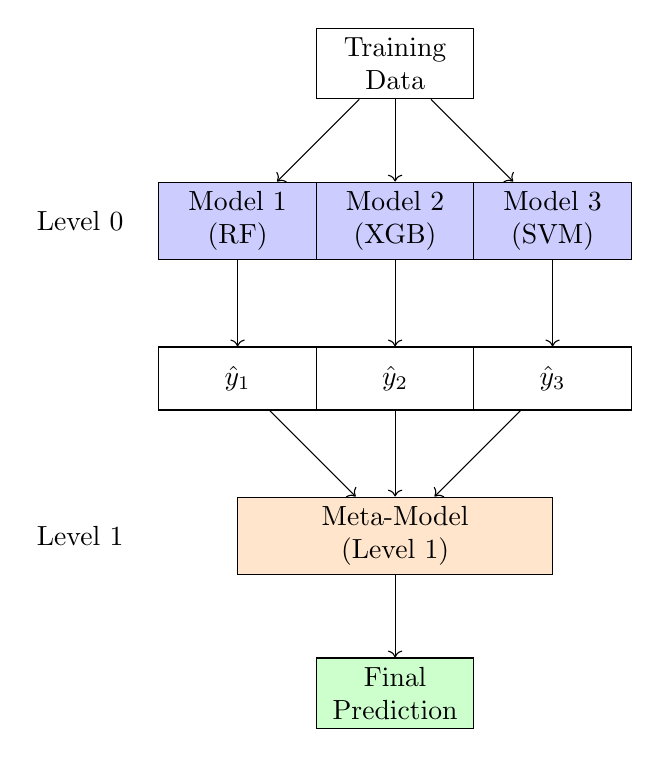
\begin{tikzpicture}[
    box/.style={rectangle, draw, minimum width=20mm, minimum height=8mm, align=center},
    level0/.style={fill=blue!20},
    level1/.style={fill=orange!20}
]
% Training data
\node[box] (data) at (0,0) {Training\\Data};

% Level 0 models
\node[box, level0] (m1) at (-2,-2) {Model 1\\(RF)};
\node[box, level0] (m2) at (0,-2) {Model 2\\(XGB)};
\node[box, level0] (m3) at (2,-2) {Model 3\\(SVM)};

% Predictions
\node[box] (p1) at (-2,-4) {$\hat{y}_1$};
\node[box] (p2) at (0,-4) {$\hat{y}_2$};
\node[box] (p3) at (2,-4) {$\hat{y}_3$};

% Meta model
\node[box, level1, minimum width=40mm] (meta) at (0,-6) {Meta-Model\\(Level 1)};

% Final prediction
\node[box, fill=green!20] (final) at (0,-8) {Final\\Prediction};

% Arrows
\draw[->] (data) -- (m1);
\draw[->] (data) -- (m2);
\draw[->] (data) -- (m3);
\draw[->] (m1) -- (p1);
\draw[->] (m2) -- (p2);
\draw[->] (m3) -- (p3);
\draw[->] (p1) -- (meta);
\draw[->] (p2) -- (meta);
\draw[->] (p3) -- (meta);
\draw[->] (meta) -- (final);

\node at (-4,-2) {Level 0};
\node at (-4,-6) {Level 1};
\end{tikzpicture}
\caption{Stacking architecture: Base models at level 0, meta-model at level 1}
\end{figure}

\subsection{Blending}

\begin{definition}[Blending]
Simplified version of stacking:
\begin{enumerate}
\item Split data: training set + hold-out validation set
\item Train base models on training set only
\item Generate predictions on hold-out set
\item Train meta-model on hold-out predictions
\end{enumerate}

Difference from stacking: Uses single hold-out set instead of cross-validation.
\end{definition}

\textbf{Blending vs Stacking}:
\begin{itemize}
\item Blending: Simpler, faster, but wastes data (hold-out not used for base model training)
\item Stacking: More complex, uses all data efficiently, more robust
\end{itemize}

\subsection{Choosing Base Models}

\begin{keyidea}
\textbf{Diversity is key}! Choose base models that make different types of errors.

\textbf{Good base model combinations}:
\begin{itemize}
\item Different algorithms: Linear models, tree-based, neural networks, SVMs
\item Different feature sets: Some models with all features, some with subsets
\item Different hyperparameters: Multiple trees with different depths
\item Different preprocessing: Some with PCA, some without; different scalings
\end{itemize}

\textbf{Poor combination}: 5 XGBoost models with similar hyperparameters (too correlated).

\textbf{Meta-model choices}:
\begin{itemize}
\item \textbf{Linear/Logistic Regression}: Simple, interpretable weights show model contributions
\item \textbf{Shallow tree}: Can capture interactions between base models
\item \textbf{Neural network}: Can learn complex combinations
\end{itemize}

Usually simple meta-models work best---base models already do the heavy lifting.
\end{keyidea}

\subsection{Practical Implementation}

\begin{implementationbox}
\textbf{Stacking in Practice}:

\begin{lstlisting}[language=Python]
from sklearn.ensemble import StackingClassifier
from sklearn.linear_model import LogisticRegression
from sklearn.ensemble import RandomForestClassifier
from xgboost import XGBClassifier
from sklearn.svm import SVC

# Define base models
base_models = [
    ('rf', RandomForestClassifier(n_estimators=100)),
    ('xgb', XGBClassifier(n_estimators=100)),
    ('svm', SVC(probability=True))
]

# Define meta-model
meta_model = LogisticRegression()

# Create stacking ensemble
stacking = StackingClassifier(
    estimators=base_models,
    final_estimator=meta_model,
    cv=5  # 5-fold CV for out-of-fold predictions
)

# Train
stacking.fit(X_train, y_train)

# Predict
y_pred = stacking.predict(X_test)
\end{lstlisting}

\textbf{Tips}:
\begin{itemize}
\item Use 5-10 fold CV for stacking
\item Include original features as inputs to meta-model (optional, often helps)
\item For competitions: Stack multiple levels (3-4 levels possible)
\item Ensure no information leakage between levels
\item Validate on completely separate test set
\end{itemize}
\end{implementationbox}

\subsection{Multi-Level Stacking}

\begin{definition}[Multi-Level Stacking]
Extend to more than 2 levels:
\begin{itemize}
\item Level 0: Many diverse base models
\item Level 1: Mid-level models on level-0 predictions
\item Level 2: Top-level meta-model on level-1 predictions
\item ... (can continue)
\end{itemize}
\end{definition}

\textbf{Caution}: Diminishing returns after 2-3 levels. More levels increase:
\begin{itemize}
\item Complexity and computational cost
\item Risk of overfitting
\item Difficulty in debugging
\end{itemize}

Used mainly in competitions where every 0.01\% matters.

\subsection{Summary of Part 3}

\begin{tcolorbox}[colback=yellow!10!white,colframe=orange!75!black,title=Key Takeaways]
\begin{enumerate}
\item \textbf{Ensemble Learning}: Combine multiple models for better performance. Three paradigms: bagging, boosting, stacking.

\item \textbf{Bagging/Random Forests}: Train models independently on bootstrap samples. Reduces variance. RF adds feature randomness. OOB error provides free validation. Excellent general-purpose algorithm.

\item \textbf{AdaBoost}: Sequential training with adaptive example weights. Focuses on hard examples. Requires weak learners better than random.

\item \textbf{Gradient Boosting}: Generalizes boosting to arbitrary losses via functional gradient descent. XGBoost, LightGBM, CatBoost are modern optimized implementations with regularization.

\item \textbf{Boosting Regularization}: Learning rate, early stopping, subsampling, tree constraints. Essential to prevent overfitting.

\item \textbf{Stacking}: Train meta-model to combine base model predictions. Use CV to generate out-of-fold predictions. Learns optimal combination weights.

\item \textbf{Model Selection}: Random Forest for robust baseline. XGBoost/LightGBM for maximum accuracy (with tuning). Stacking to combine diverse models.
\end{enumerate}

\textbf{Next Steps}: Part 4 covers neural networks and deep learning: perceptrons, backpropagation, CNNs, RNNs, Transformers, and modern optimization techniques.
\end{tcolorbox}

\begin{exercise}
\begin{enumerate}
\item Show that the probability of a specific example appearing in a bootstrap sample approaches $1 - e^{-1} \approx 0.632$ as $n \to \infty$.

\item For a Random Forest with 100 trees, each with 90\% accuracy but only 50\% correlated predictions, compute the expected ensemble accuracy if we use majority voting.

\item In AdaBoost, suppose a weak learner has error rate $\epsilon_t = 0.4$. Compute its weight $\alpha_t$. What happens if $\epsilon_t = 0.5$ (random guessing)?

\item Explain why Gradient Boosting with squared loss is equivalent to sequentially fitting residuals.

\item Design a stacking ensemble with 4 base models for a classification task. What would you choose as base models and meta-model? Justify your choices.

\item Compare computational complexity: training 100 decision trees in Random Forest vs XGBoost. Which is faster and why?

\item For XGBoost, if learning rate is 0.01, how many trees would you typically need? What if learning rate is 0.3?
\end{enumerate}
\end{exercise}

% =======================
% Part 4: Neural Networks and Deep Learning
% =======================
\addcontentsline{toc}{section}{Part 4: Neural Networks and Deep Learning}
\section*{Part 4: Neural Networks and Deep Learning}

\section{The Perceptron}

\subsection{The Perceptron Model}

\begin{definition}[Perceptron]
The perceptron is the simplest neural network unit, proposed by Rosenblatt (1958). For binary classification with $y \in \{-1, +1\}$:
\[
\hat{y} = \text{sign}(\vect{w}^\top\vect{x} + b) = \text{sign}\left(\sum_{i=1}^d w_i x_i + b\right)
\]
where $\vect{w}$ are weights, $b$ is bias, and $\text{sign}(z) = \begin{cases} +1 & z \geq 0 \\ -1 & z < 0 \end{cases}$.
\end{definition}

\begin{intuition}
The perceptron is a linear classifier: it separates data with a hyperplane. Think of it as a simplified neuron that ``fires'' (+1) when the weighted input exceeds a threshold, and doesn't fire (-1) otherwise.
\end{intuition}

\begin{figure}[H]
\centering
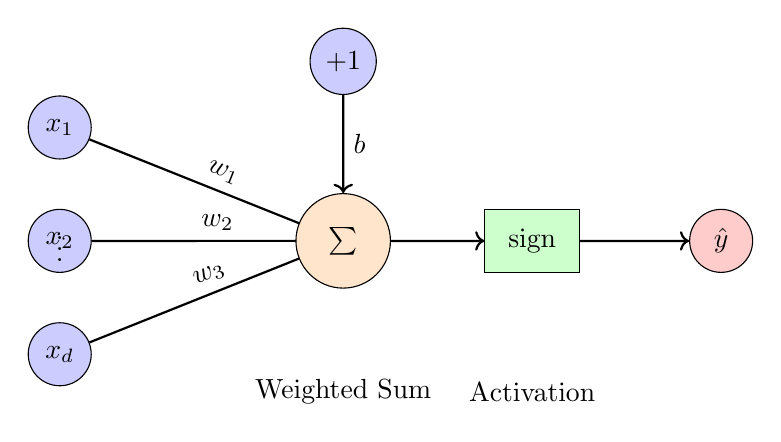
\begin{tikzpicture}[scale=1.2]
% Input nodes
\foreach \i/\label in {1/$x_1$, 2/$x_2$, 3/$x_d$} {
    \node[circle, draw, fill=blue!20, minimum size=8mm] (x\i) at (0, -\i*1.2) {\label};
}
\node at (0, -2.4) {$\vdots$};

% Weights
\foreach \i in {1,2,3} {
    \draw[->, thick] (x\i) -- (3, -2.4) node[midway, above, sloped] {$w_{\i}$};
}

% Perceptron node
\node[circle, draw, fill=orange!20, minimum size=12mm] (p) at (3, -2.4) {$\sum$};

% Activation
\node[rectangle, draw, fill=green!20, minimum width=12mm, minimum height=8mm] (a) at (5, -2.4) {sign};

% Output
\node[circle, draw, fill=red!20, minimum size=8mm] (y) at (7, -2.4) {$\hat{y}$};

% Bias
\node[circle, draw, fill=blue!20, minimum size=8mm] (b) at (3, -0.5) {$+1$};
\draw[->, thick] (b) -- (p) node[midway, right] {$b$};

% Connections
\draw[->, thick] (p) -- (a);
\draw[->, thick] (a) -- (y);

\node at (3, -4) {Weighted Sum};
\node at (5, -4) {Activation};
\end{tikzpicture}
\caption{Perceptron architecture: inputs, weights, sum, and sign activation}
\end{figure}

\subsection{Perceptron Learning Algorithm}

\begin{algorithmbox}
\textbf{Perceptron Learning Rule}

\textbf{Input}: Training data $\{(\vect{x}_i, y_i)\}_{i=1}^n$ with $y_i \in \{-1, +1\}$

\textbf{Initialize}: $\vect{w} = \vect{0}$, $b = 0$

\textbf{Repeat} until convergence (or max iterations):
\begin{enumerate}
\item For each training example $(\vect{x}_i, y_i)$:
\begin{itemize}
\item Compute prediction: $\hat{y}_i = \text{sign}(\vect{w}^\top\vect{x}_i + b)$
\item If $\hat{y}_i \neq y_i$ (misclassified):
\[
\vect{w} \leftarrow \vect{w} + y_i\vect{x}_i, \quad b \leftarrow b + y_i
\]
\end{itemize}
\end{enumerate}

\textbf{Output}: Learned weights $\vect{w}$ and bias $b$
\end{algorithmbox}

\begin{intuition}
The update rule is intuitive:
\begin{itemize}
\item If true label is $+1$ but we predicted $-1$: increase $\vect{w}$ in direction of $\vect{x}$
\item If true label is $-1$ but we predicted $+1$: decrease $\vect{w}$ in direction of $\vect{x}$
\item Correct predictions: no update
\end{itemize}
This gradually rotates the hyperplane to correctly classify examples.
\end{intuition}

\begin{theorem}[Perceptron Convergence Theorem]
If the training data is linearly separable, the perceptron learning algorithm converges in a finite number of steps. Specifically, if all examples satisfy $\norm{\vect{x}_i} \leq R$ and there exists a unit vector $\vect{w}^*$ with margin $\gamma$ such that $y_i(\vect{w}^{*\top}\vect{x}_i) \geq \gamma$ for all $i$, then the algorithm makes at most $(R/\gamma)^2$ mistakes.
\end{theorem}

\begin{proof}[Sketch]
Define mistake counter $k$. After $k$ mistakes, the weight vector is a sum of misclassified examples. Using properties of inner products and norms, one can show:
\begin{itemize}
\item Lower bound: $\vect{w}_k \cdot \vect{w}^* \geq k\gamma$ (progress toward optimal)
\item Upper bound: $\norm{\vect{w}_k}^2 \leq kR^2$ (bounded growth)
\end{itemize}
Combining via Cauchy-Schwarz: $k \leq (R/\gamma)^2$.
\end{proof}

\subsection{Limitations of the Perceptron}

\begin{keyidea}
\textbf{The XOR Problem}:

Perceptron can only learn \emph{linearly separable} functions. The XOR function is not linearly separable:

\begin{center}
\begin{tabular}{cc|c}
$x_1$ & $x_2$ & XOR \\
\hline
0 & 0 & 0 \\
0 & 1 & 1 \\
1 & 0 & 1 \\
1 & 1 & 0 \\
\end{tabular}
\end{center}

No single line can separate the 1s from the 0s!

\begin{figure}[H]
\centering
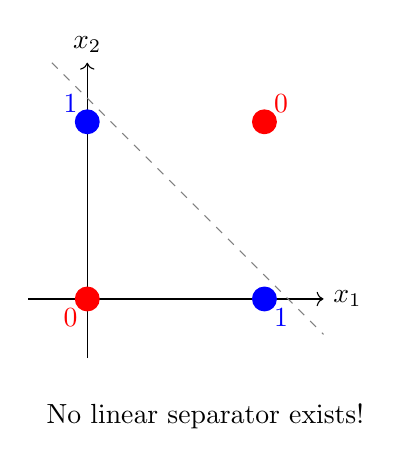
\begin{tikzpicture}[scale=1.5]
\draw[->] (-0.5,0) -- (2,0) node[right] {$x_1$};
\draw[->] (0,-0.5) -- (0,2) node[above] {$x_2$};

% XOR points
\fill[red] (0,0) circle (3pt) node[below left] {0};
\fill[blue] (0,1.5) circle (3pt) node[above left] {1};
\fill[blue] (1.5,0) circle (3pt) node[below right] {1};
\fill[red] (1.5,1.5) circle (3pt) node[above right] {0};

% Attempted separator (fails)
\draw[dashed, gray] (-0.3, 2) -- (2, -0.3);
\node at (1, -1) {No linear separator exists!};
\end{tikzpicture}
\caption{XOR is not linearly separable}
\end{figure}

\textbf{Solution}: Use multiple perceptrons in layers $\to$ Multi-Layer Perceptron (MLP) can learn XOR.

\textbf{Historical note}: This limitation caused the first ``AI winter'' in the 1970s. Minsky and Papert's book (1969) highlighted these limitations, dampening enthusiasm until backpropagation was rediscovered in the 1980s.
\end{keyidea}

% =======================
\section{Artificial Neural Networks}
% =======================

\subsection{The Neuron Model}

\begin{definition}[Artificial Neuron]
A neuron computes:
\[
a = f\left(\sum_{i=1}^d w_i x_i + b\right) = f(\vect{w}^\top\vect{x} + b)
\]
where:
\begin{itemize}
\item $\vect{x} = [x_1, \ldots, x_d]^\top$ are inputs
\item $\vect{w} = [w_1, \ldots, w_d]^\top$ are weights
\item $b$ is bias
\item $f$ is the \emph{activation function}
\item $a$ is the neuron's output (activation)
\end{itemize}
\end{definition}

\subsection{Activation Functions}

\begin{definition}[Common Activation Functions]

\textbf{1. Sigmoid}:
\[
\sigma(z) = \frac{1}{1 + e^{-z}}, \quad \sigma'(z) = \sigma(z)(1-\sigma(z))
\]
Range: $(0, 1)$. Used in output layer for binary classification.

\textbf{2. Hyperbolic Tangent (Tanh)}:
\[
\tanh(z) = \frac{e^z - e^{-z}}{e^z + e^{-z}}, \quad \tanh'(z) = 1 - \tanh^2(z)
\]
Range: $(-1, 1)$. Zero-centered (better than sigmoid for hidden layers).

\textbf{3. ReLU (Rectified Linear Unit)}:
\[
\text{ReLU}(z) = \max(0, z), \quad \text{ReLU}'(z) = \begin{cases} 1 & z > 0 \\ 0 & z \leq 0 \end{cases}
\]
Most popular for hidden layers. Fast, addresses vanishing gradient.

\textbf{4. Leaky ReLU}:
\[
\text{LeakyReLU}(z) = \max(\alpha z, z), \quad \alpha \in (0, 1) \text{ typically } 0.01
\]
Prevents ``dead neurons'' (neurons that never activate).

\textbf{5. GELU (Gaussian Error Linear Unit)}:
\[
\text{GELU}(z) = z \cdot \Phi(z)
\]
where $\Phi$ is the Gaussian CDF. Smooth, used in Transformers (BERT, GPT).

\textbf{6. Softmax} (for output layer, multi-class):
\[
\text{softmax}(\vect{z})_i = \frac{e^{z_i}}{\sum_{j=1}^K e^{z_j}}
\]
Converts logits to probability distribution.
\end{definition}

\begin{figure}[H]
\centering
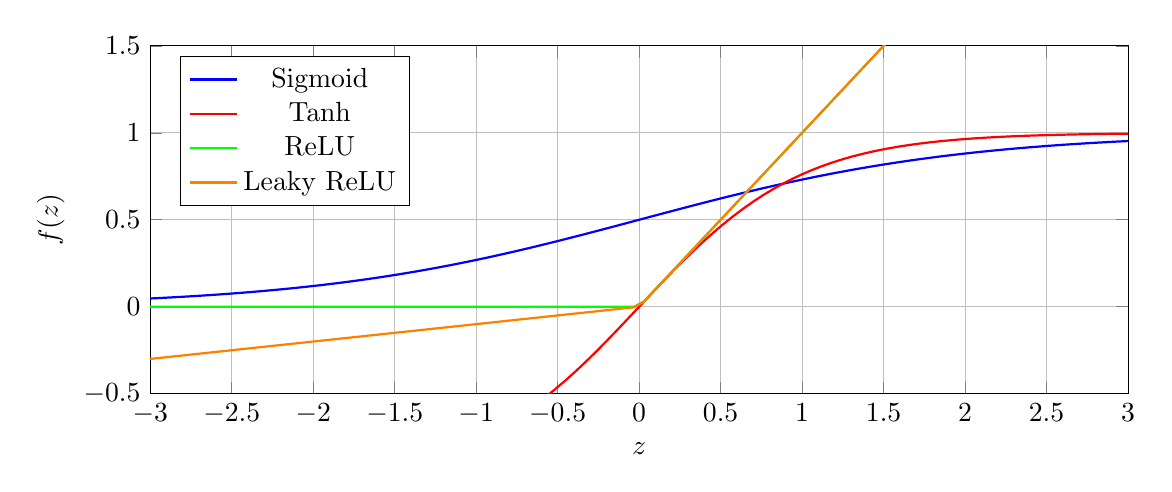
\begin{tikzpicture}
\begin{axis}[
    width=14cm,
    height=6cm,
    xlabel={$z$},
    ylabel={$f(z)$},
    xmin=-3, xmax=3,
    ymin=-0.5, ymax=1.5,
    legend pos=north west,
    grid=major
]
\addplot[blue, thick, domain=-3:3, samples=100] {1/(1+exp(-x))};
\addlegendentry{Sigmoid}

\addplot[red, thick, domain=-3:3, samples=100] {tanh(x)};
\addlegendentry{Tanh}

\addplot[green, thick, domain=-3:3, samples=100] {max(0,x)};
\addlegendentry{ReLU}

\addplot[orange, thick, domain=-3:3, samples=100] {max(0.1*x, x)};
\addlegendentry{Leaky ReLU}
\end{axis}
\end{tikzpicture}
\caption{Common activation functions}
\end{figure}

\begin{keyidea}
\textbf{Why non-linear activations?}

Without non-linearity, stacking layers is useless:
\[
f(\vect{W}_2 f(\vect{W}_1 \vect{x})) = f(\vect{W}_2 \vect{W}_1 \vect{x}) = f(\vect{W} \vect{x})
\]
Multiple linear layers collapse to a single linear transformation. Non-linear activations enable neural networks to approximate any continuous function (Universal Approximation Theorem).

\textbf{Choosing activation}:
\begin{itemize}
\item \textbf{Hidden layers}: ReLU (default), Leaky ReLU, GELU
\item \textbf{Output layer}: 
\begin{itemize}
\item Binary classification: Sigmoid
\item Multi-class: Softmax
\item Regression: Linear (no activation)
\end{itemize}
\end{itemize}
\end{keyidea}

\subsection{Multi-Layer Perceptron (MLP)}

\begin{definition}[Feedforward Neural Network]
An MLP with $L$ layers has:
\begin{itemize}
\item \textbf{Input layer}: $\vect{x} = \vect{a}^{(0)} \in \R^{d_0}$
\item \textbf{Hidden layers} $\ell = 1, \ldots, L-1$:
\[
\vect{z}^{(\ell)} = \vect{W}^{(\ell)}\vect{a}^{(\ell-1)} + \vect{b}^{(\ell)}, \quad \vect{a}^{(\ell)} = f^{(\ell)}(\vect{z}^{(\ell)})
\]
\item \textbf{Output layer} $\ell = L$:
\[
\vect{z}^{(L)} = \vect{W}^{(L)}\vect{a}^{(L-1)} + \vect{b}^{(L)}, \quad \hat{\vect{y}} = \vect{a}^{(L)} = f^{(L)}(\vect{z}^{(L)})
\]
\end{itemize}
where $\vect{W}^{(\ell)} \in \R^{d_\ell \times d_{\ell-1}}$, $\vect{b}^{(\ell)} \in \R^{d_\ell}$.
\end{definition}

\begin{figure}[H]
\centering
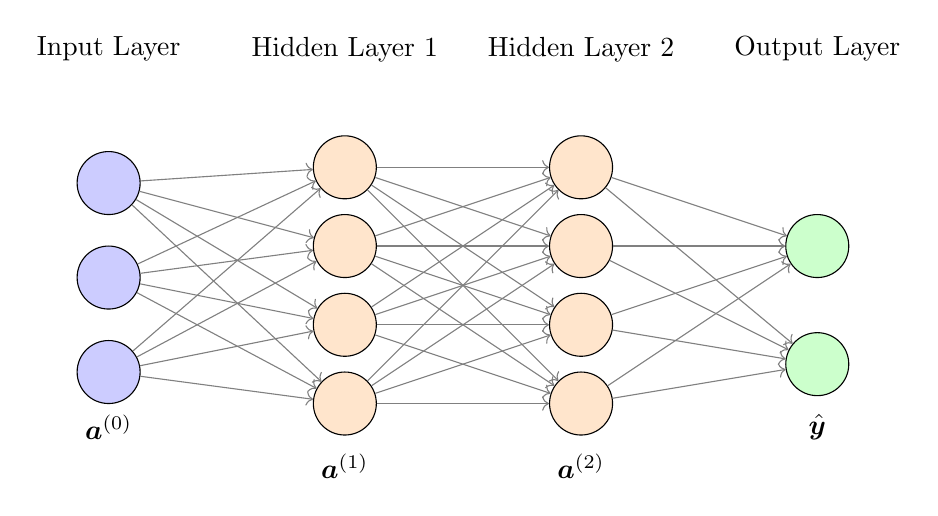
\begin{tikzpicture}[
    neuron/.style={circle, draw, minimum size=8mm, fill=blue!20},
    layer/.style={rectangle, draw=none}
]
% Input layer
\foreach \i in {1,2,3} {
    \node[neuron] (i\i) at (0, -\i*1.2) {};
}
\node[layer] at (0, 0.5) {Input Layer};
\node[layer] at (0, -4.3) {$\vect{a}^{(0)}$};

% Hidden layer 1
\foreach \i in {1,2,3,4} {
    \node[neuron, fill=orange!20] (h1\i) at (3, -\i*1) {};
}
\node[layer] at (3, 0.5) {Hidden Layer 1};
\node[layer] at (3, -4.8) {$\vect{a}^{(1)}$};

% Hidden layer 2
\foreach \i in {1,2,3,4} {
    \node[neuron, fill=orange!20] (h2\i) at (6, -\i*1) {};
}
\node[layer] at (6, 0.5) {Hidden Layer 2};
\node[layer] at (6, -4.8) {$\vect{a}^{(2)}$};

% Output layer
\foreach \i in {1,2} {
    \node[neuron, fill=green!20] (o\i) at (9, -\i*1.5-0.5) {};
}
\node[layer] at (9, 0.5) {Output Layer};
\node[layer] at (9, -4.3) {$\hat{\vect{y}}$};

% Connections (sample, not all)
\foreach \i in {1,2,3} {
    \foreach \j in {1,2,3,4} {
        \draw[->, thin, gray] (i\i) -- (h1\j);
    }
}
\foreach \i in {1,2,3,4} {
    \foreach \j in {1,2,3,4} {
        \draw[->, thin, gray] (h1\i) -- (h2\j);
    }
}
\foreach \i in {1,2,3,4} {
    \foreach \j in {1,2} {
        \draw[->, thin, gray] (h2\i) -- (o\j);
    }
}
\end{tikzpicture}
\caption{Multi-Layer Perceptron with 2 hidden layers}
\end{figure}

\subsection{Forward Propagation}

\begin{algorithmbox}
\textbf{Forward Propagation Algorithm}

\textbf{Input}: Example $\vect{x}$, network parameters $\{\vect{W}^{(\ell)}, \vect{b}^{(\ell)}\}_{\ell=1}^L$

\textbf{Initialize}: $\vect{a}^{(0)} = \vect{x}$

\textbf{For} $\ell = 1$ to $L$:
\begin{enumerate}
\item Compute pre-activation: $\vect{z}^{(\ell)} = \vect{W}^{(\ell)}\vect{a}^{(\ell-1)} + \vect{b}^{(\ell)}$
\item Compute activation: $\vect{a}^{(\ell)} = f^{(\ell)}(\vect{z}^{(\ell)})$
\end{enumerate}

\textbf{Output}: Prediction $\hat{\vect{y}} = \vect{a}^{(L)}$
\end{algorithmbox}

\subsection{Loss Functions}

\begin{definition}[Common Loss Functions]

\textbf{Regression (continuous output)}:
\begin{itemize}
\item \textbf{Mean Squared Error}: $\Loss = \frac{1}{n}\sum_{i=1}^n \norm{\vect{y}_i - \hat{\vect{y}}_i}_2^2$
\item \textbf{Mean Absolute Error}: $\Loss = \frac{1}{n}\sum_{i=1}^n \norm{\vect{y}_i - \hat{\vect{y}}_i}_1$
\end{itemize}

\textbf{Binary Classification}:
\begin{itemize}
\item \textbf{Binary Cross-Entropy}:
\[
\Loss = -\frac{1}{n}\sum_{i=1}^n [y_i\log(\hat{y}_i) + (1-y_i)\log(1-\hat{y}_i)]
\]
\end{itemize}

\textbf{Multi-Class Classification}:
\begin{itemize}
\item \textbf{Categorical Cross-Entropy}:
\[
\Loss = -\frac{1}{n}\sum_{i=1}^n \sum_{k=1}^K y_{ik}\log(\hat{y}_{ik})
\]
where $\vect{y}_i$ is one-hot encoded.
\end{itemize}
\end{definition}

\subsection{Backpropagation}

Backpropagation efficiently computes gradients using the chain rule.

\begin{theorem}[Backpropagation Algorithm]
For a network with $L$ layers, we compute gradients backward from output to input.

\textbf{Output layer gradient}:
\[
\boldsymbol{\delta}^{(L)} = \nabla_{\vect{a}^{(L)}} \Loss \odot f'^{(L)}(\vect{z}^{(L)})
\]
where $\odot$ is element-wise product.

\textbf{Hidden layer gradients} (for $\ell = L-1, L-2, \ldots, 1$):
\[
\boldsymbol{\delta}^{(\ell)} = (\vect{W}^{(\ell+1)})^\top \boldsymbol{\delta}^{(\ell+1)} \odot f'^{(\ell)}(\vect{z}^{(\ell)})
\]

\textbf{Parameter gradients}:
\[
\nabla_{\vect{W}^{(\ell)}} \Loss = \boldsymbol{\delta}^{(\ell)} (\vect{a}^{(\ell-1)})^\top, \quad \nabla_{\vect{b}^{(\ell)}} \Loss = \boldsymbol{\delta}^{(\ell)}
\]
\end{theorem}

\begin{proof}[Derivation Sketch]
By chain rule, for layer $\ell$:
\[
\pp{\Loss}{\vect{W}^{(\ell)}} = \pp{\Loss}{\vect{z}^{(\ell)}} \cdot \pp{\vect{z}^{(\ell)}}{\vect{W}^{(\ell)}}
\]
Define $\boldsymbol{\delta}^{(\ell)} = \pp{\Loss}{\vect{z}^{(\ell)}}$ (the ``error'' at layer $\ell$).

For the output layer:
\[
\boldsymbol{\delta}^{(L)} = \pp{\Loss}{\vect{a}^{(L)}} \cdot \pp{\vect{a}^{(L)}}{\vect{z}^{(L)}} = \nabla_{\vect{a}^{(L)}} \Loss \odot f'^{(L)}(\vect{z}^{(L)})
\]

For hidden layers, using chain rule through layer $\ell+1$:
\[
\boldsymbol{\delta}^{(\ell)} = \pp{\vect{z}^{(\ell+1)}}{\vect{a}^{(\ell)}} \cdot \pp{\Loss}{\vect{z}^{(\ell+1)}} \cdot \pp{\vect{a}^{(\ell)}}{\vect{z}^{(\ell)}} = (\vect{W}^{(\ell+1)})^\top \boldsymbol{\delta}^{(\ell+1)} \odot f'^{(\ell)}(\vect{z}^{(\ell)})
\]

Finally:
\[
\nabla_{\vect{W}^{(\ell)}} \Loss = \boldsymbol{\delta}^{(\ell)} (\vect{a}^{(\ell-1)})^\top
\]
\end{proof}

\begin{algorithmbox}
\textbf{Backpropagation Algorithm}

\textbf{Forward Pass}: Compute all $\vect{z}^{(\ell)}$ and $\vect{a}^{(\ell)}$ for $\ell = 1, \ldots, L$

\textbf{Backward Pass}:
\begin{enumerate}
\item Compute output error: $\boldsymbol{\delta}^{(L)} = \nabla_{\vect{a}^{(L)}} \Loss \odot f'^{(L)}(\vect{z}^{(L)})$

\item \textbf{For} $\ell = L-1$ down to $1$:
\begin{itemize}
\item Backpropagate error: $\boldsymbol{\delta}^{(\ell)} = (\vect{W}^{(\ell+1)})^\top \boldsymbol{\delta}^{(\ell+1)} \odot f'^{(\ell)}(\vect{z}^{(\ell)})$
\item Compute weight gradient: $\nabla_{\vect{W}^{(\ell)}} \Loss = \boldsymbol{\delta}^{(\ell)} (\vect{a}^{(\ell-1)})^\top$
\item Compute bias gradient: $\nabla_{\vect{b}^{(\ell)}} \Loss = \boldsymbol{\delta}^{(\ell)}$
\end{itemize}
\end{enumerate}

\textbf{Update}: $\vect{W}^{(\ell)} \leftarrow \vect{W}^{(\ell)} - \eta \nabla_{\vect{W}^{(\ell)}} \Loss$ for all layers
\end{algorithmbox}

\begin{keyidea}
\textbf{Why backpropagation is efficient}:

Naive approach: Compute each partial derivative independently $\to$ $O(n \cdot p)$ where $p$ is number of parameters.

Backpropagation: Compute all gradients in one backward pass $\to$ $O(p)$, roughly the same as one forward pass.

The key insight: Reuse intermediate computations. The error $\boldsymbol{\delta}^{(\ell)}$ at layer $\ell$ depends on $\boldsymbol{\delta}^{(\ell+1)}$, so we propagate errors backward efficiently.
\end{keyidea}

\subsection{Vanishing and Exploding Gradients}

\begin{definition}[Gradient Vanishing]
In deep networks with sigmoid/tanh activations, gradients can become very small as they propagate backward, making early layers learn very slowly.

\textbf{Why?} $\sigma'(z) = \sigma(z)(1-\sigma(z)) \leq 0.25$. For a network with $L$ layers:
\[
\pp{\Loss}{\vect{W}^{(1)}} \propto \prod_{\ell=1}^L \sigma'(z^{(\ell)}) \vect{W}^{(\ell)}
\]
If $\sigma'(z) \approx 0.1$, then gradient $\approx 0.1^L \to 0$ exponentially fast.
\end{definition}

\begin{definition}[Gradient Exploding]
Conversely, if weights are large or activations unbounded, gradients can explode:
\[
\text{gradient} \propto \prod_{\ell} \vect{W}^{(\ell)} \to \infty
\]
Causes numerical instability, NaN values.
\end{definition}

\begin{keyidea}
\textbf{Solutions to Vanishing/Exploding Gradients}:

\textbf{1. Better Activation Functions}:
\begin{itemize}
\item ReLU: $f'(z) = 1$ for $z > 0$ (no vanishing in positive region)
\item Leaky ReLU, ELU: Address ``dying ReLU'' problem
\end{itemize}

\textbf{2. Careful Weight Initialization}:
\begin{itemize}
\item Xavier/Glorot: $\vect{W} \sim \mathcal{N}(0, 2/(d_{\text{in}} + d_{\text{out}}))$
\item He initialization (for ReLU): $\vect{W} \sim \mathcal{N}(0, 2/d_{\text{in}})$
\end{itemize}

\textbf{3. Batch Normalization}: Normalize activations at each layer

\textbf{4. Residual Connections} (ResNet): Skip connections allow gradients to flow directly

\textbf{5. Gradient Clipping}: Cap gradients at a maximum value (for exploding)

\textbf{6. LSTM/GRU}: Specifically designed for RNNs to address vanishing gradients
\end{keyidea}

% =======================
\section{Optimization in Deep Learning}
% =======================

\subsection{Stochastic Gradient Descent Variants}

\subsubsection{Momentum}

\begin{definition}[SGD with Momentum]
Accumulate past gradients to accelerate convergence:
\[
\vect{v}_t = \beta \vect{v}_{t-1} + \eta \nabla_{\vect{w}} \Loss, \quad \vect{w}_{t+1} = \vect{w}_t - \vect{v}_t
\]
Typical: $\beta = 0.9$. Alternatively, some formulations use $\vect{v}_t = \beta \vect{v}_{t-1} + \nabla_{\vect{w}} \Loss$ with $\vect{w}_{t+1} = \vect{w}_t - \eta \vect{v}_t$.
\end{definition}

\begin{intuition}
Momentum accelerates in directions with consistent gradients and dampens oscillations. Think of a ball rolling down a hill---it builds up speed in the downhill direction.
\end{intuition}

\subsubsection{RMSProp}

\begin{definition}[RMSProp (Root Mean Square Propagation)]
Adapt learning rate per parameter using moving average of squared gradients:
\[
\vect{s}_t = \beta \vect{s}_{t-1} + (1-\beta)(\nabla_{\vect{w}} \Loss)^2, \quad \vect{w}_{t+1} = \vect{w}_t - \frac{\eta}{\sqrt{\vect{s}_t + \epsilon}} \odot \nabla_{\vect{w}} \Loss
\]
Typical: $\beta = 0.9$, $\epsilon = 10^{-8}$.
\end{definition}

\begin{intuition}
RMSProp divides the learning rate by a running average of the gradient magnitude. Parameters with large gradients get smaller effective learning rates; parameters with small gradients get larger effective rates. This helps with different scales across parameters.
\end{intuition}

\subsubsection{Adam}

\begin{definition}[Adam (Adaptive Moment Estimation)]
Combines momentum and RMSProp:
\begin{align}
\vect{m}_t &= \beta_1 \vect{m}_{t-1} + (1-\beta_1)\nabla_{\vect{w}} \Loss && \text{(first moment)} \\
\vect{v}_t &= \beta_2 \vect{v}_{t-1} + (1-\beta_2)(\nabla_{\vect{w}} \Loss)^2 && \text{(second moment)} \\
\hat{\vect{m}}_t &= \frac{\vect{m}_t}{1 - \beta_1^t}, \quad \hat{\vect{v}}_t = \frac{\vect{v}_t}{1 - \beta_2^t} && \text{(bias correction)} \\
\vect{w}_{t+1} &= \vect{w}_t - \frac{\eta}{\sqrt{\hat{\vect{v}}_t} + \epsilon} \odot \hat{\vect{m}}_t
\end{align}
Typical: $\beta_1 = 0.9$, $\beta_2 = 0.999$, $\eta = 0.001$, $\epsilon = 10^{-8}$.
\end{definition}

\begin{keyidea}
\textbf{Adam is the default optimizer for deep learning}:
\begin{itemize}
\item Combines benefits of momentum (acceleration) and RMSProp (adaptive rates)
\item Works well across a wide range of problems
\item Bias correction ensures good estimates early in training
\item Relatively insensitive to hyperparameters
\end{itemize}

\textbf{Variants}:
\begin{itemize}
\item \textbf{AdamW}: Adam with decoupled weight decay (better regularization)
\item \textbf{AMSGrad}: Fixes potential convergence issues in Adam
\item \textbf{Nadam}: Nesterov + Adam
\end{itemize}
\end{keyidea}

\subsection{Learning Rate Schedules}

\begin{definition}[Learning Rate Decay Strategies]

\textbf{1. Step Decay}:
\[
\eta_t = \eta_0 \cdot \gamma^{\lfloor t / k \rfloor}
\]
Drop learning rate by factor $\gamma$ every $k$ epochs.

\textbf{2. Exponential Decay}:
\[
\eta_t = \eta_0 e^{-\lambda t}
\]

\textbf{3. Cosine Annealing}:
\[
\eta_t = \eta_{\min} + \frac{1}{2}(\eta_{\max} - \eta_{\min})\left(1 + \cos\left(\frac{t}{T}\pi\right)\right)
\]
Smoothly decreases from $\eta_{\max}$ to $\eta_{\min}$ over $T$ steps.

\textbf{4. Warm-up + Decay}:
\begin{itemize}
\item Linearly increase LR from 0 to $\eta_0$ over first few epochs (warm-up)
\item Then apply decay schedule
\end{itemize}
Used in Transformers.
\end{definition}

\subsection{Batch Normalization}

\begin{definition}[Batch Normalization]
For a mini-batch $\mathcal{B} = \{\vect{x}_1, \ldots, \vect{x}_m\}$, normalize each feature:
\begin{align}
\mu_{\mathcal{B}} &= \frac{1}{m}\sum_{i=1}^m x_i \\
\sigma_{\mathcal{B}}^2 &= \frac{1}{m}\sum_{i=1}^m (x_i - \mu_{\mathcal{B}})^2 \\
\hat{x}_i &= \frac{x_i - \mu_{\mathcal{B}}}{\sqrt{\sigma_{\mathcal{B}}^2 + \epsilon}} \\
y_i &= \gamma \hat{x}_i + \beta
\end{align}
where $\gamma$ and $\beta$ are learnable parameters (scale and shift).
\end{definition}

\begin{keyidea}
\textbf{Benefits of Batch Normalization}:
\begin{itemize}
\item \textbf{Faster training}: Can use higher learning rates
\item \textbf{Reduces internal covariate shift}: Stabilizes distribution of layer inputs
\item \textbf{Regularization effect}: Adds noise (batch statistics), reduces overfitting
\item \textbf{Less sensitive to initialization}: Makes training more robust
\end{itemize}

\textbf{Where to apply}: After linear transformation, before activation:
\[
\vect{z} = \vect{W}\vect{a}^{(\ell-1)} + \vect{b} \to \text{BatchNorm}(\vect{z}) \to f(\cdot)
\]

\textbf{At test time}: Use running averages of $\mu$ and $\sigma^2$ computed during training (no batch available).
\end{keyidea}

\subsection{Dropout}

\begin{definition}[Dropout]
During training, randomly set activations to zero with probability $p$ (typically 0.5):
\[
\tilde{a}_i = \begin{cases}
0 & \text{with probability } p \\
a_i / (1-p) & \text{with probability } 1-p
\end{cases}
\]
At test time, use all neurons (no dropout).
\end{definition}

\begin{intuition}
Dropout prevents co-adaptation of neurons. By randomly dropping neurons, the network cannot rely on any specific neurons, forcing it to learn robust features. It's like training an ensemble of networks that share weights.
\end{intuition}

\begin{keyidea}
\textbf{Dropout as Regularization}:
\begin{itemize}
\item Prevents overfitting, especially in fully-connected layers
\item Typical $p$: 0.2-0.5 for hidden layers, 0-0.2 for input layer
\item Not typically used in convolutional layers (they have fewer parameters)
\item Can be viewed as approximate Bayesian inference
\end{itemize}

\textbf{Variants}:
\begin{itemize}
\item \textbf{DropConnect}: Drop weights instead of activations
\item \textbf{Spatial Dropout}: For CNNs, drop entire feature maps
\end{itemize}
\end{keyidea}

% =======================
\section{Deep Architectures}
% =======================

\subsection{Convolutional Neural Networks (CNNs)}

\subsubsection{Motivation for CNNs}

\textbf{Problem with fully-connected networks for images}:
\begin{itemize}
\item Image $32 \times 32 \times 3$ has 3072 pixels. Hidden layer with 1000 neurons $\to$ 3M parameters just in first layer!
\item No spatial structure: treats pixels far apart the same as nearby pixels
\item Not translation invariant: must learn same feature at every location
\end{itemize}

\textbf{CNNs exploit}:
\begin{itemize}
\item \textbf{Local connectivity}: Neurons connect to small spatial regions
\item \textbf{Weight sharing}: Same filter applied across entire image
\item \textbf{Translation equivariance}: Features detected anywhere in the image
\end{itemize}

\subsubsection{Convolutional Layer}

\begin{definition}[Convolution Operation]
For input $\vect{X} \in \R^{H \times W \times C}$ and filter $\vect{K} \in \R^{F \times F \times C}$:
\[
Y[i,j] = \sum_{di=0}^{F-1}\sum_{dj=0}^{F-1}\sum_{c=1}^C X[i+di, j+dj, c] \cdot K[di, dj, c] + b
\]
Apply this for all positions $(i,j)$ to get feature map $\vect{Y}$.

With $D$ filters, output has shape $(H', W', D)$ where:
\[
H' = \frac{H - F + 2P}{S} + 1, \quad W' = \frac{W - F + 2P}{S} + 1
\]
$P$ = padding, $S$ = stride.
\end{definition}

\begin{figure}[H]
\centering
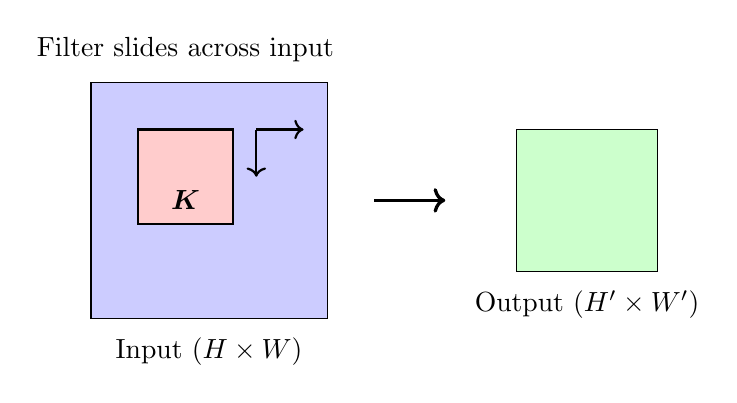
\begin{tikzpicture}[scale=0.6]
% Input
\draw[fill=blue!20] (0,0) rectangle (5,5);
\node at (2.5, -0.7) {Input $(H \times W)$};

% Filter
\draw[fill=red!20, thick] (1,2) rectangle (3,4);
\node at (2, 2.5) {$\vect{K}$};
\draw[->, very thick] (6, 2.5) -- (7.5, 2.5);

% Output
\draw[fill=green!20] (9,1) rectangle (12,4);
\node at (10.5, 0.3) {Output $(H' \times W')$};

% Annotations
\node at (2, 5.7) {Filter slides across input};
\draw[->, thick] (3.5, 4) -- (4.5, 4);
\draw[->, thick] (3.5, 4) -- (3.5, 3);
\end{tikzpicture}
\caption{Convolution operation: filter slides across input to produce output feature map}
\end{figure}

\begin{keyidea}
\textbf{Key Concepts}:

\textbf{1. Receptive Field}: Region of input that affects one output neuron. Deeper layers have larger receptive fields.

\textbf{2. Padding}:
\begin{itemize}
\item \textbf{Valid} (no padding): Output size decreases
\item \textbf{Same} (pad to maintain size): $P = (F-1)/2$ for stride 1
\end{itemize}

\textbf{3. Stride}: Step size. Larger stride $\to$ smaller output, reduces computation.

\textbf{4. Number of Parameters}: For filter $F \times F \times C$ with $D$ filters:
\[
\text{params} = (F \times F \times C + 1) \times D
\]
Much smaller than fully-connected layer!
\end{keyidea}

\subsubsection{Pooling Layers}

\begin{definition}[Pooling]
Downsampling operation to reduce spatial dimensions:

\textbf{Max Pooling}: Take maximum in each region
\[
Y[i,j] = \max_{di,dj} X[i \cdot S + di, j \cdot S + dj]
\]

\textbf{Average Pooling}: Take average
\[
Y[i,j] = \frac{1}{F^2}\sum_{di,dj} X[i \cdot S + di, j \cdot S + dj]
\]

Common: $2 \times 2$ pooling with stride 2 (halves dimensions).
\end{definition}

\textbf{Benefits of pooling}:
\begin{itemize}
\item Reduces computation and memory
\item Provides translation invariance
\item Increases receptive field
\end{itemize}

\subsubsection{Common CNN Architectures}

\begin{example}[LeNet-5 (1998) - Digit Recognition]
\texttt{Input (32×32) → Conv(6 filters, 5×5) → Pool(2×2) → Conv(16 filters, 5×5) → Pool(2×2) → FC(120) → FC(84) → FC(10)}

First successful CNN, used for ZIP code recognition.
\end{example}

\begin{example}[AlexNet (2012) - ImageNet Winner]
\begin{itemize}
\item 8 layers (5 conv, 3 FC)
\item ReLU activation (first major use)
\item Dropout for regularization
\item Data augmentation
\item 60M parameters, reduced top-5 error from 26\% to 15.3\%
\end{itemize}
Marked the beginning of the deep learning revolution.
\end{example}

\begin{example}[VGGNet (2014)]
\begin{itemize}
\item Very deep (16-19 layers)
\item Only $3 \times 3$ convolutions (smaller filters, stacked)
\item Showed depth is crucial
\item 138M parameters (VGG-16)
\end{itemize}
\end{example}

\begin{example}[ResNet (2015) - 152 Layers]
\textbf{Key innovation: Residual Connections}

Instead of learning $\mathcal{H}(\vect{x})$, learn residual $\mathcal{F}(\vect{x})$ where:
\[
\mathcal{H}(\vect{x}) = \mathcal{F}(\vect{x}) + \vect{x}
\]
Skip connections allow gradients to flow directly, enabling very deep networks.

Won ImageNet 2015, error rate 3.6\% (below human performance!).
\end{example}

\begin{figure}[H]
\centering
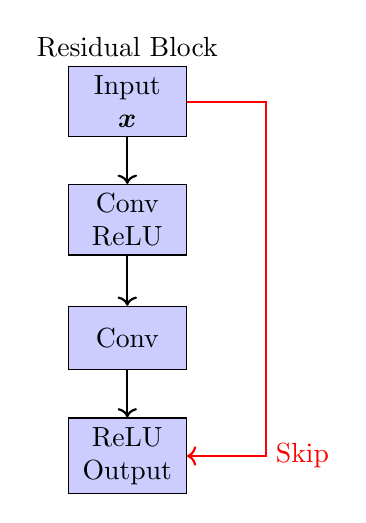
\begin{tikzpicture}[
    block/.style={rectangle, draw, minimum width=15mm, minimum height=8mm, align=center},
    conv/.style={fill=blue!20},
    fc/.style={fill=green!20}
]
% ResNet block
\node[block, conv] (in) at (0,0) {Input\\$\vect{x}$};
\node[block, conv] (c1) at (0,-1.5) {Conv\\ReLU};
\node[block, conv] (c2) at (0,-3) {Conv};
\node[block, conv] (out) at (0,-4.5) {ReLU\\Output};

% Skip connection
\draw[->, thick] (in) -- (c1);
\draw[->, thick] (c1) -- (c2);
\draw[->, thick] (c2) -- (out);
\draw[->, thick, red] (in.east) -- ++(1,0) |- (out.east) node[midway, right] {Skip};

\node at (0, 0.7) {Residual Block};
\end{tikzpicture}
\caption{ResNet residual block with skip connection}
\end{figure}

\subsection{Recurrent Neural Networks (RNNs)}

\subsubsection{Sequence Modeling}

\textbf{Motivation}: Many problems involve sequences:
\begin{itemize}
\item Text: ``The cat sat on the \_\_\_'' (predict next word)
\item Time series: Stock prices, weather data
\item Speech: Audio to text
\item Video: Frame-by-frame analysis
\end{itemize}

\textbf{Challenge}: Variable-length inputs and dependencies between timesteps.

\subsubsection{Vanilla RNN}

\begin{definition}[Recurrent Neural Network]
At timestep $t$:
\begin{align}
\vect{h}_t &= f(\vect{W}_{hh}\vect{h}_{t-1} + \vect{W}_{xh}\vect{x}_t + \vect{b}_h) \\
\vect{y}_t &= \vect{W}_{hy}\vect{h}_t + \vect{b}_y
\end{align}
where:
\begin{itemize}
\item $\vect{x}_t$: input at time $t$
\item $\vect{h}_t$: hidden state (memory)
\item $\vect{y}_t$: output at time $t$
\item $f$: activation (typically tanh or ReLU)
\end{itemize}
\end{definition}

\begin{figure}[H]
\centering
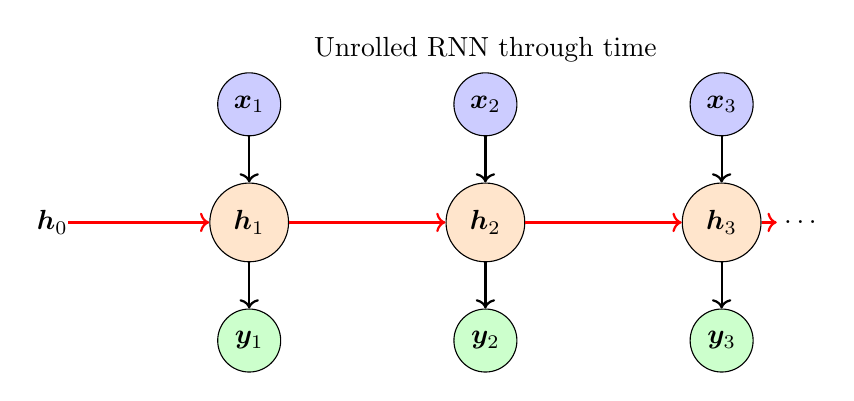
\begin{tikzpicture}[
    neuron/.style={circle, draw, minimum size=10mm, fill=orange!20},
    input/.style={circle, draw, minimum size=8mm, fill=blue!20},
    output/.style={circle, draw, minimum size=8mm, fill=green!20}
]
% Time steps
\foreach \t in {1,2,3} {
    \node[input] (x\t) at (\t*3, 0) {$\vect{x}_{\t}$};
    \node[neuron] (h\t) at (\t*3, -1.5) {$\vect{h}_{\t}$};
    \node[output] (y\t) at (\t*3, -3) {$\vect{y}_{\t}$};
    
    \draw[->, thick] (x\t) -- (h\t);
    \draw[->, thick] (h\t) -- (y\t);
    
    \ifnum\t>1
        \draw[->, thick, red] (h\the\numexpr\t-1) -- (h\t);
    \fi
}

\node at (0.5, -1.5) {$\vect{h}_0$};
\draw[->, thick, red] (0.7, -1.5) -- (h1);
\draw[->, thick, red] (h3) -- ++(0.7, 0);
\node at (10, -1.5) {$\ldots$};

\node at (6, 0.7) {Unrolled RNN through time};
\end{tikzpicture}
\caption{RNN unrolled through time. Red arrows show recurrent connections.}
\end{figure}

\subsubsection{Backpropagation Through Time (BPTT)}

Training RNNs: Unfold network through time and apply backpropagation. Gradients flow backward through all timesteps.

\textbf{Problem}: Vanishing gradients are even worse in RNNs!
\[
\pp{\Loss}{\vect{h}_1} \propto \prod_{t=2}^T \pp{\vect{h}_t}{\vect{h}_{t-1}} = \prod_{t=2}^T \vect{W}_{hh} \cdot f'(\vect{z}_t)
\]
For long sequences ($T$ large), gradient vanishes or explodes exponentially.

\subsubsection{LSTM (Long Short-Term Memory)}

\begin{definition}[LSTM Cell]
LSTM uses gates to control information flow:

\textbf{Forget gate}: What to forget from cell state
\[
\vect{f}_t = \sigma(\vect{W}_f[\vect{h}_{t-1}, \vect{x}_t] + \vect{b}_f)
\]

\textbf{Input gate}: What new information to add
\[
\vect{i}_t = \sigma(\vect{W}_i[\vect{h}_{t-1}, \vect{x}_t] + \vect{b}_i)
\]
\[
\tilde{\vect{c}}_t = \tanh(\vect{W}_c[\vect{h}_{t-1}, \vect{x}_t] + \vect{b}_c)
\]

\textbf{Cell state update}:
\[
\vect{c}_t = \vect{f}_t \odot \vect{c}_{t-1} + \vect{i}_t \odot \tilde{\vect{c}}_t
\]

\textbf{Output gate}: What to output
\[
\vect{o}_t = \sigma(\vect{W}_o[\vect{h}_{t-1}, \vect{x}_t] + \vect{b}_o)
\]
\[
\vect{h}_t = \vect{o}_t \odot \tanh(\vect{c}_t)
\]
\end{definition}

\begin{keyidea}
\textbf{Why LSTM works}:
\begin{itemize}
\item Cell state $\vect{c}_t$ acts as a ``conveyor belt'' for information
\item Gates (sigmoid $\in [0,1]$) control what flows through
\item Forget gate can preserve gradients over long sequences
\item Addresses vanishing gradient problem
\end{itemize}

\textbf{When to use LSTM}:
\begin{itemize}
\item Long sequences (>50-100 timesteps)
\item Long-term dependencies matter
\item Text generation, machine translation, speech recognition
\end{itemize}
\end{keyidea}

\subsubsection{GRU (Gated Recurrent Unit)}

\begin{definition}[GRU]
Simplified version of LSTM with fewer parameters:

\textbf{Update gate}:
\[
\vect{z}_t = \sigma(\vect{W}_z[\vect{h}_{t-1}, \vect{x}_t])
\]

\textbf{Reset gate}:
\[
\vect{r}_t = \sigma(\vect{W}_r[\vect{h}_{t-1}, \vect{x}_t])
\]

\textbf{Candidate hidden state}:
\[
\tilde{\vect{h}}_t = \tanh(\vect{W}[\vect{r}_t \odot \vect{h}_{t-1}, \vect{x}_t])
\]

\textbf{Hidden state update}:
\[
\vect{h}_t = (1 - \vect{z}_t) \odot \vect{h}_{t-1} + \vect{z}_t \odot \tilde{\vect{h}}_t
\]
\end{definition}

\textbf{GRU vs LSTM}:
\begin{itemize}
\item GRU: Simpler, fewer parameters, faster training
\item LSTM: More expressive, better for very long sequences
\item Performance often similar---try both!
\end{itemize}

\subsection{Transformers and Attention}

\subsubsection{Limitations of RNNs}

\begin{itemize}
\item \textbf{Sequential computation}: Cannot parallelize (must process $t-1$ before $t$)
\item \textbf{Long-range dependencies}: Still struggle despite LSTM/GRU
\item \textbf{Fixed hidden state}: Must compress entire history into $\vect{h}_t$
\end{itemize}

\textbf{Solution}: Attention mechanism---directly access any part of the input.

\subsubsection{Attention Mechanism}

\begin{definition}[Attention]
Given query $\vect{q}$, keys $\vect{K} = [\vect{k}_1, \ldots, \vect{k}_n]$, and values $\vect{V} = [\vect{v}_1, \ldots, \vect{v}_n]$:

\textbf{1. Compute attention scores}:
\[
e_i = \text{score}(\vect{q}, \vect{k}_i)
\]
Common: $\text{score}(\vect{q}, \vect{k}) = \vect{q}^\top\vect{k}$ (dot product)

\textbf{2. Normalize to get attention weights}:
\[
\alpha_i = \frac{\exp(e_i)}{\sum_j \exp(e_j)} \quad \text{(softmax)}
\]

\textbf{3. Compute weighted sum}:
\[
\text{context} = \sum_{i=1}^n \alpha_i \vect{v}_i
\]
\end{definition}

\begin{intuition}
Attention allows the model to ``focus'' on relevant parts of the input. For translation, when generating word $t$, attention looks at all source words and focuses on the most relevant ones.
\end{intuition}

\subsubsection{Scaled Dot-Product Attention}

\begin{definition}[Scaled Dot-Product Attention]
\[
\text{Attention}(\vect{Q}, \vect{K}, \vect{V}) = \text{softmax}\left(\frac{\vect{Q}\vect{K}^\top}{\sqrt{d_k}}\right)\vect{V}
\]
where $\vect{Q} \in \R^{n \times d_k}$, $\vect{K} \in \R^{m \times d_k}$, $\vect{V} \in \R^{m \times d_v}$.

Scaling by $\sqrt{d_k}$ prevents softmax saturation for large $d_k$.
\end{definition}

\subsubsection{Transformer Architecture}

\begin{definition}[Transformer (Vaswani et al., 2017)]
Uses only attention mechanisms (no recurrence):

\textbf{Key components}:
\begin{enumerate}
\item \textbf{Multi-Head Attention}: Multiple attention operations in parallel
\[
\text{MultiHead}(\vect{Q}, \vect{K}, \vect{V}) = \text{Concat}(\text{head}_1, \ldots, \text{head}_h)\vect{W}^O
\]
where $\text{head}_i = \text{Attention}(\vect{Q}\vect{W}_i^Q, \vect{K}\vect{W}_i^K, \vect{V}\vect{W}_i^V)$

\item \textbf{Positional Encoding}: Add position information (since no recurrence)
\[
PE_{(pos, 2i)} = \sin(pos/10000^{2i/d}), \quad PE_{(pos, 2i+1)} = \cos(pos/10000^{2i/d})
\]

\item \textbf{Feed-Forward Networks}: Applied position-wise
\[
\text{FFN}(\vect{x}) = \max(0, \vect{x}\vect{W}_1 + \vect{b}_1)\vect{W}_2 + \vect{b}_2
\]

\item \textbf{Layer Normalization} and \textbf{Residual Connections}
\end{enumerate}
\end{definition}

\begin{keyidea}
\textbf{Why Transformers Revolutionized NLP}:
\begin{itemize}
\item \textbf{Parallelization}: All positions processed simultaneously
\item \textbf{Long-range dependencies}: Direct connections between any positions
\item \textbf{Scalability}: Can train on massive datasets efficiently
\item \textbf{Transfer learning}: Pre-train on large corpus, fine-tune on task
\end{itemize}

\textbf{Impact}:
\begin{itemize}
\item BERT (2018): Bidirectional Transformer for language understanding
\item GPT series (2018-2023): Decoder-only Transformers for generation
\item Vision Transformers (ViT): Applied to images
\item Now the dominant architecture in NLP and increasingly in vision
\end{itemize}
\end{keyidea}

\subsection{Summary of Part 4}

\begin{tcolorbox}[colback=yellow!10!white,colframe=orange!75!black,title=Key Takeaways]
\begin{enumerate}
\item \textbf{Perceptron}: First neural network model. Linear classifier with convergence guarantee for separable data. Cannot learn XOR (not linearly separable).

\item \textbf{MLPs}: Stack layers with non-linear activations. Universal approximators. Trained via backpropagation---efficient gradient computation using chain rule.

\item \textbf{Activation Functions}: ReLU is default for hidden layers (addresses vanishing gradients). Sigmoid/Softmax for output. GELU in modern architectures.

\item \textbf{Optimization}: Adam is standard optimizer. Learning rate schedules improve convergence. Batch normalization and dropout for regularization.

\item \textbf{CNNs}: Exploit spatial structure via convolution and pooling. Weight sharing reduces parameters. ResNet's skip connections enable very deep networks.

\item \textbf{RNNs}: Process sequences with recurrent connections. Vanilla RNNs suffer from vanishing gradients. LSTM/GRU use gates to maintain long-term memory.

\item \textbf{Transformers}: Attention mechanism allows direct access to all inputs. Fully parallelizable, handles long-range dependencies. Dominant architecture in modern NLP and increasingly in vision.
\end{enumerate}

\textbf{Next Steps}: Part 5 explores unsupervised learning: clustering, dimensionality reduction, and methods for discovering structure without labels.
\end{tcolorbox}

\begin{exercise}
\begin{enumerate}
\item Prove that a single-layer perceptron cannot learn the XOR function. Show that a two-layer network with 2 hidden neurons can learn it.

\item Derive the backpropagation equations for a 3-layer network with sigmoid activations and MSE loss.

\item For a conv layer with input $32 \times 32 \times 3$, filter size $5 \times 5$, 64 filters, stride 1, padding 2: compute output dimensions and number of parameters.

\item Explain why ReLU helps with vanishing gradients compared to sigmoid. What is the ``dying ReLU'' problem?

\item Implement gradient descent with momentum by hand for $f(x) = x^2$, starting from $x_0 = 10$, with $\eta = 0.1$, $\beta = 0.9$. Show 5 iterations.

\item In an LSTM, what happens if the forget gate outputs all 1s? All 0s?

\item For scaled dot-product attention with $d_k = 64$, why do we divide by $\sqrt{64} = 8$? What happens without scaling?

\item Compare computational complexity: training a 10-layer RNN vs a 10-layer Transformer on a sequence of length 100. Which is faster and why?
\end{enumerate}
\end{exercise}

% =======================
% Part 5: Unsupervised Learning
% =======================
\addcontentsline{toc}{section}{Part 5: Unsupervised Learning}
\section*{Part 5: Unsupervised Learning}

\section{Introduction to Unsupervised Learning}

\begin{definition}[Unsupervised Learning]
In unsupervised learning, we have only input data $\mathcal{D} = \{\vect{x}_1, \vect{x}_2, \ldots, \vect{x}_n\}$ without labels. The goal is to discover hidden structure or patterns in the data.
\end{definition}

\begin{keyidea}
\textbf{Main Tasks in Unsupervised Learning}:

\begin{itemize}
\item \textbf{Clustering}: Group similar examples together
\item \textbf{Dimensionality Reduction}: Find lower-dimensional representations
\item \textbf{Density Estimation}: Model the probability distribution $P(\vect{x})$
\item \textbf{Anomaly Detection}: Identify unusual or outlier examples
\item \textbf{Association Rules}: Discover relationships between variables
\end{itemize}

\textbf{Why Unsupervised Learning?}
\begin{itemize}
\item Labeled data is expensive; unlabeled data is abundant
\item Discover hidden structures humans might miss
\item Preprocessing for supervised learning (feature extraction)
\item Understand data distribution and relationships
\end{itemize}
\end{keyidea}

% =======================
\section{Clustering}
% =======================

\subsection{K-Means Clustering}

\subsubsection{Problem Formulation}

\begin{definition}[K-Means Objective]
Given data $\{\vect{x}_i\}_{i=1}^n$ and desired number of clusters $K$, find:
\begin{itemize}
\item Cluster centers (centroids) $\{\vect{\mu}_k\}_{k=1}^K$
\item Cluster assignments $\{c_i\}_{i=1}^n$ where $c_i \in \{1, \ldots, K\}$
\end{itemize}
to minimize within-cluster sum of squares:
\[
J = \sum_{i=1}^n \norm{\vect{x}_i - \vect{\mu}_{c_i}}_2^2 = \sum_{k=1}^K \sum_{i: c_i=k} \norm{\vect{x}_i - \vect{\mu}_k}_2^2
\]
\end{definition}

\begin{intuition}
K-means finds $K$ cluster centers and assigns each point to its nearest center. The objective minimizes the total distance from points to their assigned centers---we want tight, compact clusters.
\end{intuition}

\subsubsection{Lloyd's Algorithm}

\begin{algorithmbox}
\textbf{K-Means Algorithm (Lloyd's Algorithm)}

\textbf{Input}: Data $\{\vect{x}_i\}_{i=1}^n$, number of clusters $K$, max iterations $T$

\textbf{Initialize}: Randomly select $K$ points as initial centroids $\{\vect{\mu}_k\}_{k=1}^K$

\textbf{Repeat} until convergence (or $T$ iterations):
\begin{enumerate}
\item \textbf{Assignment step}: Assign each point to nearest centroid
\[
c_i = \argmin_{k \in \{1,\ldots,K\}} \norm{\vect{x}_i - \vect{\mu}_k}_2^2
\]

\item \textbf{Update step}: Recompute centroids as mean of assigned points
\[
\vect{\mu}_k = \frac{1}{|C_k|}\sum_{i \in C_k} \vect{x}_i
\]
where $C_k = \{i : c_i = k\}$ is the set of points assigned to cluster $k$.

\item \textbf{Check convergence}: If assignments don't change, stop
\end{enumerate}

\textbf{Output}: Cluster centers $\{\vect{\mu}_k\}$ and assignments $\{c_i\}$
\end{algorithmbox}

\begin{theorem}[K-Means Convergence]
Lloyd's algorithm is guaranteed to converge to a local minimum of $J$. The objective decreases (or stays the same) at each iteration:
\begin{itemize}
\item Assignment step: Each point moves to nearest center $\to$ $J$ decreases
\item Update step: Each center moves to mean of its cluster $\to$ $J$ decreases
\end{itemize}
Since $J \geq 0$ and there are finitely many possible assignments, the algorithm must converge.
\end{theorem}

\begin{figure}[H]
\centering
\begin{tikzpicture}[scale=0.9]
% Initial data points
\foreach \point in {(1,1), (1.5,1.2), (1.2,0.8), (5,1), (5.5,1.3), (5.2,0.9), (3,4), (3.5,4.2), (3.2,3.8)} {
    \fill[blue] \point circle (2pt);
}

% Initial centroids
\fill[red] (2,2) circle (4pt);
\fill[red] (4,1) circle (4pt);
\fill[red] (3,3) circle (4pt);
\node at (3, -0.5) {Iteration 0: Random init};

% After iteration 1
\begin{scope}[shift={(8,0)}]
\foreach \point in {(1,1), (1.5,1.2), (1.2,0.8)} {
    \fill[blue!50] \point circle (2pt);
}
\foreach \point in {(5,1), (5.5,1.3), (5.2,0.9)} {
    \fill[green!50] \point circle (2pt);
}
\foreach \point in {(3,4), (3.5,4.2), (3.2,3.8)} {
    \fill[orange!50] \point circle (2pt);
}

\fill[red] (1.23,1) circle (4pt);
\fill[red] (5.23,1.07) circle (4pt);
\fill[red] (3.23,4) circle (4pt);
\node at (3, -0.5) {Iteration 1: Converged};
\end{scope}
\end{tikzpicture}
\caption{K-Means iterations: Initial random centroids converge to cluster centers}
\end{figure}

\begin{keyidea}
\textbf{Initialization Matters!}

K-means finds a \emph{local} minimum, which depends on initialization.

\textbf{K-Means++ Initialization}:
\begin{enumerate}
\item Choose first center uniformly at random
\item For each subsequent center, choose point with probability proportional to squared distance from nearest existing center
\item Repeat until $K$ centers chosen
\end{enumerate}

This spreads out initial centers, leading to better final clusters.

\textbf{Multiple Runs}: Run K-means multiple times (10-100) with different initializations, keep the best result (lowest $J$).
\end{keyidea}

\subsubsection{Choosing K (Number of Clusters)}

\begin{definition}[Elbow Method]
Plot $J$ (within-cluster sum of squares) vs $K$. Look for an ``elbow''---a point where $J$ stops decreasing rapidly.

\begin{figure}[H]
\centering
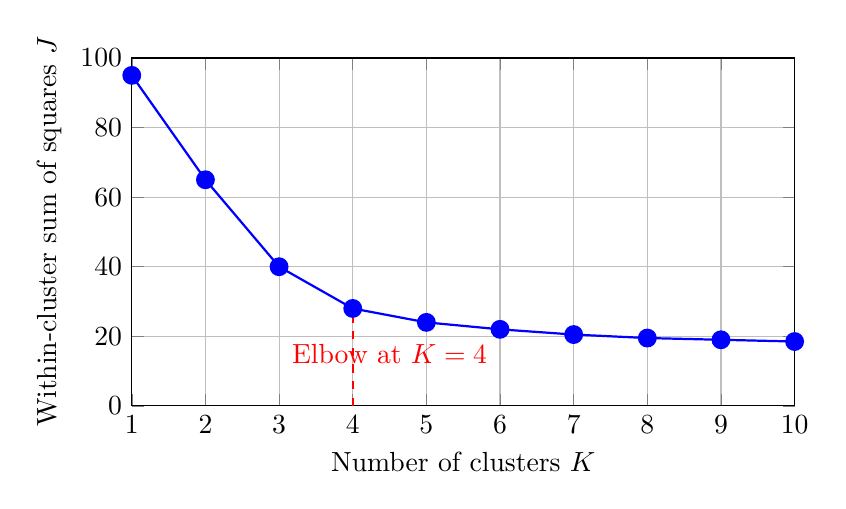
\begin{tikzpicture}
\begin{axis}[
    width=10cm,
    height=6cm,
    xlabel={Number of clusters $K$},
    ylabel={Within-cluster sum of squares $J$},
    xmin=1, xmax=10,
    ymin=0, ymax=100,
    xtick={1,2,3,4,5,6,7,8,9,10},
    grid=major
]
\addplot[blue, thick, mark=*, mark size=3pt] coordinates {
    (1,95) (2,65) (3,40) (4,28) (5,24) (6,22) (7,20.5) (8,19.5) (9,19) (10,18.5)
};
\draw[red, dashed, thick] (axis cs:4,0) -- (axis cs:4,28);
\node[red] at (axis cs:4.5,15) {Elbow at $K=4$};
\end{axis}
\end{tikzpicture}
\caption{Elbow method: $J$ decreases rapidly until $K=4$, then flattens}
\end{figure}
\end{definition}

\begin{definition}[Silhouette Score]
For each point $i$, compute:
\begin{itemize}
\item $a_i$: Average distance to other points in same cluster
\item $b_i$: Average distance to points in nearest other cluster
\end{itemize}
Silhouette coefficient:
\[
s_i = \frac{b_i - a_i}{\max(a_i, b_i)} \in [-1, 1]
\]
\begin{itemize}
\item $s_i \approx 1$: Well clustered (far from other clusters)
\item $s_i \approx 0$: On boundary between clusters
\item $s_i < 0$: Possibly assigned to wrong cluster
\end{itemize}

\textbf{Silhouette score}: Average $s_i$ over all points. Higher is better.
\end{definition}

\subsubsection{Advantages and Limitations}

\begin{keyidea}
\textbf{Advantages of K-Means}:
\begin{itemize}
\item Simple, intuitive, easy to implement
\item Fast: $O(nKdT)$ where $T$ is number of iterations (usually small)
\item Scales to large datasets
\item Works well for spherical, well-separated clusters
\end{itemize}

\textbf{Limitations}:
\begin{itemize}
\item Must specify $K$ in advance
\item Assumes spherical clusters of similar size
\item Sensitive to outliers
\item Sensitive to initialization (local minima)
\item Only uses Euclidean distance
\item Poor with non-convex cluster shapes
\end{itemize}

\textbf{Variants}:
\begin{itemize}
\item \textbf{K-Medoids}: Use actual data points as centers (more robust to outliers)
\item \textbf{Fuzzy C-Means}: Soft assignments (points can belong to multiple clusters)
\item \textbf{K-Means||}: Parallelizable version for big data
\end{itemize}
\end{keyidea}

\subsection{Hierarchical Clustering}

\begin{definition}[Hierarchical Clustering]
Build a tree (dendrogram) of nested clusters. Two approaches:
\begin{itemize}
\item \textbf{Agglomerative (bottom-up)}: Start with each point as its own cluster, merge closest pairs
\item \textbf{Divisive (top-down)}: Start with all points in one cluster, recursively split
\end{itemize}
Agglomerative is more common.
\end{definition}

\subsubsection{Agglomerative Clustering}

\begin{algorithmbox}
\textbf{Agglomerative Hierarchical Clustering}

\textbf{Input}: Data $\{\vect{x}_i\}_{i=1}^n$, linkage criterion

\textbf{Initialize}: Each point is its own cluster: $C_i = \{\vect{x}_i\}$ for $i=1,\ldots,n$

\textbf{Repeat} until one cluster remains:
\begin{enumerate}
\item Find the two closest clusters $C_i$ and $C_j$ according to linkage criterion
\item Merge them: $C_{\text{new}} = C_i \cup C_j$
\item Remove $C_i$ and $C_j$, add $C_{\text{new}}$
\end{enumerate}

\textbf{Output}: Dendrogram (tree of merges)
\end{algorithmbox}

\begin{definition}[Linkage Criteria]
How to measure distance between clusters?

\textbf{1. Single Linkage} (minimum):
\[
d(C_i, C_j) = \min_{\vect{x} \in C_i, \vect{z} \in C_j} \norm{\vect{x} - \vect{z}}
\]
Distance between closest points. Tends to create long, chain-like clusters.

\textbf{2. Complete Linkage} (maximum):
\[
d(C_i, C_j) = \max_{\vect{x} \in C_i, \vect{z} \in C_j} \norm{\vect{x} - \vect{z}}
\]
Distance between farthest points. Creates compact, spherical clusters.

\textbf{3. Average Linkage}:
\[
d(C_i, C_j) = \frac{1}{|C_i||C_j|}\sum_{\vect{x} \in C_i}\sum_{\vect{z} \in C_j} \norm{\vect{x} - \vect{z}}
\]
Average distance between all pairs.

\textbf{4. Ward's Method}:
Minimize increase in within-cluster variance when merging. Most popular choice.
\[
d(C_i, C_j) = \frac{|C_i||C_j|}{|C_i| + |C_j|} \norm{\vect{\mu}_i - \vect{\mu}_j}^2
\]
\end{definition}

\begin{figure}[H]
\centering
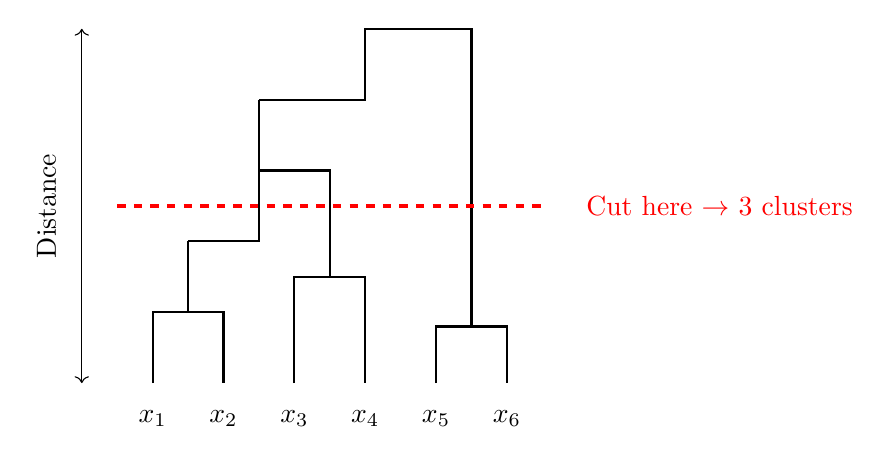
\begin{tikzpicture}[scale=0.9]
% Dendrogram
\draw[thick] (0,0) -- (0,1) -- (1,1) -- (1,0);
\draw[thick] (0.5,1) -- (0.5,2);
\draw[thick] (2,0) -- (2,1.5) -- (3,1.5) -- (3,0);
\draw[thick] (2.5,1.5) -- (2.5,2);
\draw[thick] (0.5,2) -- (1.5,2) -- (1.5,3) -- (2.5,3) -- (2.5,2);
\draw[thick] (1.5,3) -- (1.5,4);
\draw[thick] (4,0) -- (4,0.8) -- (5,0.8) -- (5,0);
\draw[thick] (4.5,0.8) -- (4.5,4);
\draw[thick] (1.5,4) -- (3,4) -- (3,5) -- (4.5,5) -- (4.5,4);

% Cut line
\draw[red, dashed, very thick] (-0.5, 2.5) -- (5.5, 2.5);
\node[red] at (8, 2.5) {Cut here $\to$ 3 clusters};

% Labels
\node at (0, -0.5) {$x_1$};
\node at (1, -0.5) {$x_2$};
\node at (2, -0.5) {$x_3$};
\node at (3, -0.5) {$x_4$};
\node at (4, -0.5) {$x_5$};
\node at (5, -0.5) {$x_6$};

\draw[<->] (-1, 0) -- (-1, 5);
\node[rotate=90] at (-1.5, 2.5) {Distance};
\end{tikzpicture}
\caption{Dendrogram: Hierarchical clustering tree. Cut at different heights for different $K$.}
\end{figure}

\begin{keyidea}
\textbf{Advantages of Hierarchical Clustering}:
\begin{itemize}
\item No need to specify $K$ in advance
\item Dendrogram provides full hierarchy
\item Deterministic (no random initialization)
\item Can handle any distance metric
\item Intuitive visualization
\end{itemize}

\textbf{Limitations}:
\begin{itemize}
\item \textbf{Computational cost}: $O(n^3)$ time, $O(n^2)$ space
\item Cannot scale to large datasets (millions of points)
\item Greedy: Cannot undo merges
\item Sensitive to noise and outliers
\end{itemize}

\textbf{When to use}:
\begin{itemize}
\item Small to medium datasets ($n < 10,000$)
\item When you want to explore different numbers of clusters
\item When hierarchy itself is meaningful (taxonomy, phylogenetic trees)
\end{itemize}
\end{keyidea}

\subsection{DBSCAN (Density-Based Clustering)}

\begin{definition}[DBSCAN]
DBSCAN (Density-Based Spatial Clustering of Applications with Noise) clusters based on density. Two parameters:
\begin{itemize}
\item $\epsilon$: Neighborhood radius
\item $\text{minPts}$: Minimum points to form a dense region
\end{itemize}

\textbf{Point types}:
\begin{itemize}
\item \textbf{Core point}: Has $\geq \text{minPts}$ points within distance $\epsilon$
\item \textbf{Border point}: Within $\epsilon$ of a core point, but not core itself
\item \textbf{Noise point}: Neither core nor border
\end{itemize}
\end{definition}

\begin{algorithmbox}
\textbf{DBSCAN Algorithm}

\textbf{Input}: Data $\{\vect{x}_i\}$, $\epsilon$, $\text{minPts}$

\textbf{Initialize}: All points unmarked, cluster counter $C = 0$

\textbf{For} each unmarked point $\vect{x}_i$:
\begin{enumerate}
\item Find $N_\epsilon(\vect{x}_i) = \{\vect{x}_j : \norm{\vect{x}_i - \vect{x}_j} \leq \epsilon\}$ (neighbors)
\item \textbf{If} $|N_\epsilon(\vect{x}_i)| < \text{minPts}$: 
\begin{itemize}
\item Mark $\vect{x}_i$ as noise (for now)
\end{itemize}
\item \textbf{Else} ($\vect{x}_i$ is core point):
\begin{itemize}
\item $C = C + 1$ (new cluster)
\item Mark $\vect{x}_i$ with cluster $C$
\item Initialize queue $Q = N_\epsilon(\vect{x}_i)$
\item \textbf{While} $Q$ not empty:
\begin{itemize}
\item Pop $\vect{x}_j$ from $Q$
\item If $\vect{x}_j$ was noise: mark with cluster $C$ (border point)
\item If $\vect{x}_j$ unmarked: mark with cluster $C$
\item If $\vect{x}_j$ is core point: add its neighbors to $Q$
\end{itemize}
\end{itemize}
\end{enumerate}

\textbf{Output}: Cluster assignments (or noise label)
\end{algorithmbox}

\begin{figure}[H]
\centering
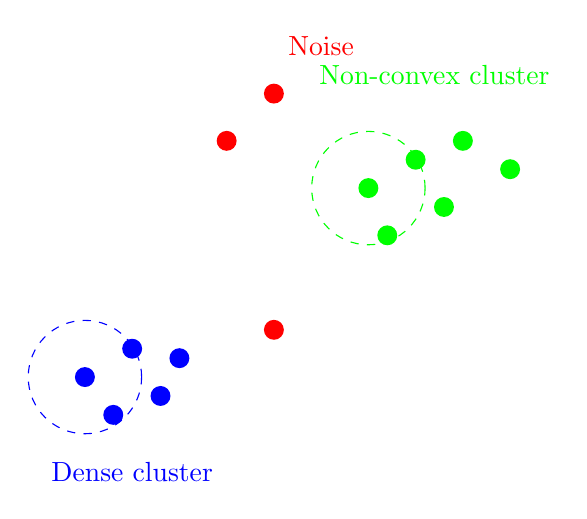
\begin{tikzpicture}[scale=1.2]
% Cluster 1
\foreach \point in {(0,0), (0.5,0.3), (0.3,-0.4), (1,0.2), (0.8,-0.2)} {
    \fill[blue] \point circle (3pt);
}

% Cluster 2 (crescent shape)
\foreach \point in {(3,2), (3.5,2.3), (3.2,1.5), (3.8,1.8), (4,2.5), (4.5,2.2)} {
    \fill[green] \point circle (3pt);
}

% Noise points
\fill[red] (2,0.5) circle (3pt);
\fill[red] (1.5,2.5) circle (3pt);
\fill[red] (2,3) circle (3pt);

% Epsilon circles (examples)
\draw[blue, dashed] (0,0) circle (0.6);
\draw[green, dashed] (3,2) circle (0.6);

\node[blue] at (0.5, -1) {Dense cluster};
\node[green] at (3.7, 3.2) {Non-convex cluster};
\node[red] at (2.5, 3.5) {Noise};
\end{tikzpicture}
\caption{DBSCAN finds arbitrarily-shaped clusters and identifies outliers as noise}
\end{figure}

\begin{keyidea}
\textbf{Advantages of DBSCAN}:
\begin{itemize}
\item \textbf{Discovers arbitrary shapes}: Not limited to spherical clusters
\item \textbf{Handles noise}: Explicitly identifies outliers
\item \textbf{No need to specify $K$}: Number of clusters determined automatically
\item \textbf{Only two parameters}: $\epsilon$ and minPts
\end{itemize}

\textbf{Limitations}:
\begin{itemize}
\item Sensitive to $\epsilon$ and minPts (hard to tune)
\item Struggles with varying densities
\item $O(n^2)$ complexity (can use KD-trees to reduce to $O(n\log n)$)
\item Border points can be assigned arbitrarily if equidistant to multiple clusters
\end{itemize}

\textbf{Parameter selection}:
\begin{itemize}
\item \textbf{minPts}: Often set to $2d$ where $d$ is dimensionality, or 4-5 for 2D data
\item \textbf{$\epsilon$}: Plot k-distance graph (distance to $k$-th nearest neighbor), look for ``knee''
\end{itemize}
\end{keyidea}

\subsection{Cluster Evaluation Metrics}

When ground truth labels are unavailable:

\begin{definition}[Davies-Bouldin Index]
\[
\text{DB} = \frac{1}{K}\sum_{i=1}^K \max_{j \neq i} \left(\frac{s_i + s_j}{d_{ij}}\right)
\]
where $s_i$ is average distance within cluster $i$, and $d_{ij}$ is distance between cluster centers.

\textbf{Lower is better} (smaller within-cluster spread, larger between-cluster separation).
\end{definition}

\begin{definition}[Calinski-Harabasz Index (Variance Ratio)]
\[
\text{CH} = \frac{\text{Between-cluster variance}}{\text{Within-cluster variance}} \cdot \frac{n - K}{K - 1}
\]
\textbf{Higher is better} (better separation).
\end{definition}

When ground truth labels are available:

\begin{definition}[Adjusted Rand Index (ARI)]
Measures agreement between predicted clusters and true labels, adjusted for chance.
\[
\text{ARI} \in [-1, 1]
\]
\begin{itemize}
\item ARI = 1: Perfect agreement
\item ARI = 0: Random assignment
\item ARI < 0: Worse than random
\end{itemize}
\end{definition}

% =======================
\section{Dimensionality Reduction}
% =======================

\subsection{Motivation}

\begin{keyidea}
\textbf{The Curse of Dimensionality}:
\begin{itemize}
\item Data in high dimensions is sparse (most volume in corners of hypercube)
\item Distance metrics become less meaningful
\item Overfitting becomes severe
\item Computational cost grows exponentially
\end{itemize}

\textbf{Benefits of Dimensionality Reduction}:
\begin{itemize}
\item Visualization (reduce to 2D or 3D)
\item Noise reduction (eliminate irrelevant features)
\item Faster training (fewer features)
\item Storage efficiency
\item Avoid overfitting
\end{itemize}

\textbf{Two approaches}:
\begin{itemize}
\item \textbf{Feature Selection}: Select subset of original features
\item \textbf{Feature Extraction}: Create new features as combinations of originals
\end{itemize}
\end{keyidea}

\subsection{Principal Component Analysis (PCA)}

\subsubsection{Intuition and Formulation}

\begin{definition}[PCA Goal]
Find a low-dimensional linear subspace that captures maximum variance in the data.

Formally, find $k$ orthogonal directions $\{\vect{u}_1, \ldots, \vect{u}_k\}$ that maximize:
\[
\max_{\vect{u}_1, \ldots, \vect{u}_k} \sum_{j=1}^k \Var(\vect{x}^\top \vect{u}_j)
\]
subject to $\norm{\vect{u}_j} = 1$ and $\vect{u}_i \perp \vect{u}_j$ for $i \neq j$.
\end{definition}

\begin{intuition}
PCA finds new coordinate axes (principal components) along which data has maximum spread. The first component captures the most variance, the second captures the most remaining variance (orthogonal to the first), and so on.

Think of a 3D cloud of points shaped like a pancake. PCA finds the plane that best fits the pancake, and potentially a line within that plane.
\end{intuition}

\begin{theorem}[PCA via Eigendecomposition]
Given centered data (mean subtracted), the principal components are the eigenvectors of the covariance matrix $\mat{\Sigma} = \frac{1}{n}\mat{X}^\top\mat{X}$.

\textbf{Steps}:
\begin{enumerate}
\item Center data: $\tilde{\vect{x}}_i = \vect{x}_i - \bar{\vect{x}}$ where $\bar{\vect{x}} = \frac{1}{n}\sum_i \vect{x}_i$
\item Compute covariance: $\mat{\Sigma} = \frac{1}{n}\sum_{i=1}^n \tilde{\vect{x}}_i\tilde{\vect{x}}_i^\top$
\item Eigendecomposition: $\mat{\Sigma} = \mat{U}\mat{\Lambda}\mat{U}^\top$
\item Sort eigenvalues $\lambda_1 \geq \lambda_2 \geq \cdots \geq \lambda_d$
\item Top $k$ eigenvectors $\{\vect{u}_1, \ldots, \vect{u}_k\}$ are principal components
\end{enumerate}

\textbf{Projection}: $\vect{z}_i = \mat{U}_k^\top \tilde{\vect{x}}_i \in \R^k$ where $\mat{U}_k = [\vect{u}_1, \ldots, \vect{u}_k]$.

\textbf{Reconstruction}: $\hat{\vect{x}}_i = \mat{U}_k \vect{z}_i + \bar{\vect{x}}$.
\end{theorem}

\begin{proof}[Sketch]
We want to maximize $\sum_i (\vect{u}_1^\top \tilde{\vect{x}}_i)^2 = \vect{u}_1^\top \left(\sum_i \tilde{\vect{x}}_i\tilde{\vect{x}}_i^\top\right)\vect{u}_1 = \vect{u}_1^\top \mat{\Sigma} \vect{u}_1$.

Using Lagrange multipliers for constraint $\norm{\vect{u}_1} = 1$:
\[
\mathcal{L} = \vect{u}_1^\top \mat{\Sigma} \vect{u}_1 - \lambda(\vect{u}_1^\top\vect{u}_1 - 1)
\]
Taking derivative and setting to zero:
\[
\mat{\Sigma}\vect{u}_1 = \lambda\vect{u}_1
\]
So $\vect{u}_1$ is an eigenvector of $\mat{\Sigma}$. To maximize variance, choose eigenvector with largest eigenvalue $\lambda_1$. The variance captured is $\lambda_1$. Repeat for subsequent components (orthogonal eigenvectors).
\end{proof}

\begin{algorithmbox}
\textbf{PCA Algorithm}

\textbf{Input}: Data $\mat{X} \in \R^{n \times d}$, target dimension $k$

\begin{enumerate}
\item Center data: $\tilde{\mat{X}} = \mat{X} - \bar{\vect{x}}\mathbf{1}^\top$ where $\bar{\vect{x}} = \frac{1}{n}\sum_i \vect{x}_i$
\item Compute covariance: $\mat{\Sigma} = \frac{1}{n}\tilde{\mat{X}}^\top\tilde{\mat{X}}$
\item Compute eigenvectors/eigenvalues: $\mat{\Sigma} = \mat{U}\mat{\Lambda}\mat{U}^\top$
\item Sort eigenvalues in descending order
\item Select top $k$ eigenvectors: $\mat{U}_k = [\vect{u}_1, \ldots, \vect{u}_k]$
\item Project data: $\mat{Z} = \tilde{\mat{X}}\mat{U}_k$
\end{enumerate}

\textbf{Output}: Reduced data $\mat{Z} \in \R^{n \times k}$, transformation $\mat{U}_k$
\end{algorithmbox}

\subsubsection{Choosing Number of Components}

\begin{definition}[Explained Variance Ratio]
Proportion of total variance captured by first $k$ components:
\[
\text{EVR}_k = \frac{\sum_{j=1}^k \lambda_j}{\sum_{j=1}^d \lambda_j}
\]
Common threshold: Keep enough components to explain 90-95\% of variance.
\end{definition}

\begin{figure}[H]
\centering
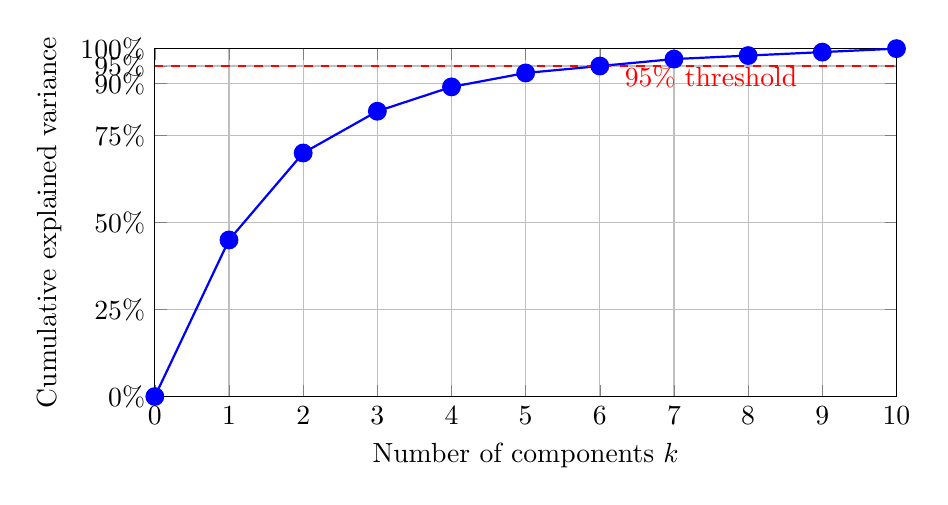
\begin{tikzpicture}
\begin{axis}[
    width=11cm,
    height=6cm,
    xlabel={Number of components $k$},
    ylabel={Cumulative explained variance},
    xmin=0, xmax=10,
    ymin=0, ymax=1,
    ytick={0, 0.25, 0.5, 0.75, 0.9, 0.95, 1},
    yticklabels={0\%, 25\%, 50\%, 75\%, 90\%, 95\%, 100\%},
    grid=major,
    legend pos=south east
]
\addplot[blue, thick, mark=*, mark size=3pt] coordinates {
    (0,0) (1,0.45) (2,0.70) (3,0.82) (4,0.89) (5,0.93) (6,0.95) (7,0.97) (8,0.98) (9,0.99) (10,1.0)
};
\draw[red, dashed] (axis cs:0,0.95) -- (axis cs:10,0.95);
\node[red] at (axis cs:7.5, 0.92) {95\% threshold};
\end{axis}
\end{tikzpicture}
\caption{Scree plot: Cumulative explained variance vs number of components}
\end{figure}

\subsubsection{PCA Properties and Limitations}

\begin{keyidea}
\textbf{Key Properties of PCA}:
\begin{itemize}
\item \textbf{Linear transformation}: $\vect{z} = \mat{U}_k^\top(\vect{x} - \bar{\vect{x}})$
\item \textbf{Optimal reconstruction}: Minimizes reconstruction error $\sum_i \norm{\vect{x}_i - \hat{\vect{x}}_i}^2$
\item \textbf{Uncorrelated components}: $\Cov(\vect{z}_i, \vect{z}_j) = 0$ for $i \neq j$
\item \textbf{Ordered by importance}: First component captures most variance
\end{itemize}

\textbf{Advantages}:
\begin{itemize}
\item Fast, closed-form solution (eigendecomposition)
\item Interpretable (variance explained)
\item No hyperparameters (except $k$)
\item Reversible (can reconstruct)
\end{itemize}

\textbf{Limitations}:
\begin{itemize}
\item \textbf{Linear only}: Cannot capture non-linear structure
\item \textbf{Assumes variance = importance}: High variance might be noise
\item \textbf{Sensitive to scaling}: Must standardize features first
\item \textbf{Assumes Gaussian distribution}: Works best for normally distributed data
\item \textbf{Interpretability}: Components are linear combinations, hard to interpret
\end{itemize}

\textbf{When to use PCA}:
\begin{itemize}
\item Preprocessing for supervised learning
\item Visualization (project to 2D/3D)
\item Noise reduction
\item When features are correlated
\end{itemize}
\end{keyidea}

\subsection{Linear Discriminant Analysis (LDA)}

\begin{definition}[LDA]
Unlike PCA (unsupervised), LDA is \emph{supervised} dimensionality reduction. It finds directions that maximize separation between classes.

\textbf{Goal}: Find projection $\vect{w}$ that maximizes:
\[
J(\vect{w}) = \frac{\text{Between-class variance}}{\text{Within-class variance}} = \frac{\vect{w}^\top \mat{S}_B \vect{w}}{\vect{w}^\top \mat{S}_W \vect{w}}
\]
where:
\begin{itemize}
\item $\mat{S}_W = \sum_{c=1}^K \sum_{i \in C_c} (\vect{x}_i - \vect{\mu}_c)(\vect{x}_i - \vect{\mu}_c)^\top$ (within-class scatter)
\item $\mat{S}_B = \sum_{c=1}^K n_c (\vect{\mu}_c - \vect{\mu})(\vect{\mu}_c - \vect{\mu})^\top$ (between-class scatter)
\end{itemize}
\end{definition}

\begin{theorem}[LDA Solution]
Optimal projection directions are eigenvectors of $\mat{S}_W^{-1}\mat{S}_B$ corresponding to largest eigenvalues.

Maximum number of components: $\min(d, K-1)$ where $K$ is number of classes.
\end{theorem}

\begin{keyidea}
\textbf{PCA vs LDA}:
\begin{itemize}
\item \textbf{PCA}: Unsupervised, maximizes variance, uses all data
\item \textbf{LDA}: Supervised, maximizes class separation, uses labels
\end{itemize}

\textbf{When to use LDA}:
\begin{itemize}
\item Dimensionality reduction before classification
\item When classes are well-separated
\item When you have class labels
\end{itemize}

LDA often gives better results for classification tasks because it uses label information.
\end{keyidea}

\subsection{Non-Linear Methods}

\subsubsection{t-SNE (t-Distributed Stochastic Neighbor Embedding)}

\begin{definition}[t-SNE]
Non-linear method that preserves local structure. Particularly good for visualization.

\textbf{Idea}:
\begin{enumerate}
\item In high-dimensional space, compute pairwise similarities:
\[
p_{ij} = \frac{\exp(-\norm{\vect{x}_i - \vect{x}_j}^2 / 2\sigma^2)}{\sum_{k \neq l} \exp(-\norm{\vect{x}_k - \vect{x}_l}^2 / 2\sigma^2)}
\]

\item In low-dimensional space, use t-distribution:
\[
q_{ij} = \frac{(1 + \norm{\vect{z}_i - \vect{z}_j}^2)^{-1}}{\sum_{k \neq l} (1 + \norm{\vect{z}_k - \vect{z}_l}^2)^{-1}}
\]

\item Minimize KL divergence: $\text{KL}(P||Q) = \sum_{i,j} p_{ij}\log\frac{p_{ij}}{q_{ij}}$
\end{enumerate}

Optimized via gradient descent.
\end{definition}

\begin{keyidea}
\textbf{t-SNE Properties}:
\begin{itemize}
\item Excellent for visualization (clusters become very clear)
\item Preserves local structure (nearby points stay nearby)
\item Non-linear (can capture complex manifolds)
\item Stochastic (different runs give different results)
\item \textbf{Cannot be applied to new data} (no explicit mapping, must rerun)
\item Computationally expensive: $O(n^2)$
\item Hyperparameter sensitive (perplexity, learning rate)
\end{itemize}

\textbf{When to use}:
\begin{itemize}
\item Visualization of high-dimensional data
\item Exploratory analysis
\item \textbf{Not for preprocessing} (use PCA for that)
\end{itemize}

\textbf{Interpretation caution}:
\begin{itemize}
\item Cluster sizes don't mean anything
\item Distances between clusters don't mean anything
\item Only local structure (within clusters) is meaningful
\end{itemize}
\end{keyidea}

\subsubsection{UMAP (Uniform Manifold Approximation and Projection)}

\begin{definition}[UMAP]
Similar goal to t-SNE but with better theoretical foundation (Riemannian geometry and algebraic topology).

\textbf{Advantages over t-SNE}:
\begin{itemize}
\item Faster ($O(n)$ vs $O(n^2)$)
\item Better preserves global structure
\item Can be applied to new data (unlike t-SNE)
\item Scales to larger datasets
\item Often better separation of clusters
\end{itemize}

Popular for single-cell RNA-seq visualization and other large-scale applications.
\end{definition}

\subsubsection{Autoencoders}

\begin{definition}[Autoencoder]
Neural network that learns to compress and reconstruct data.

\textbf{Architecture}:
\begin{itemize}
\item \textbf{Encoder}: $\vect{z} = f_{\text{enc}}(\vect{x}; \vect{\theta}_{\text{enc}})$ maps $\vect{x} \in \R^d$ to $\vect{z} \in \R^k$ (bottleneck)
\item \textbf{Decoder}: $\hat{\vect{x}} = f_{\text{dec}}(\vect{z}; \vect{\theta}_{\text{dec}})$ reconstructs from $\vect{z}$
\end{itemize}

\textbf{Training}: Minimize reconstruction error:
\[
\Loss = \sum_{i=1}^n \norm{\vect{x}_i - \hat{\vect{x}}_i}^2
\]
\end{definition}

\begin{keyidea}
\textbf{Types of Autoencoders}:
\begin{itemize}
\item \textbf{Undercomplete}: Bottleneck $k < d$ (forced to compress)
\item \textbf{Sparse}: Regularize activations in bottleneck
\item \textbf{Denoising}: Train to reconstruct from corrupted input
\item \textbf{Variational (VAE)}: Learn probability distribution in latent space (generative model)
\end{itemize}

\textbf{Advantages}:
\begin{itemize}
\item Non-linear (can capture complex structure)
\item Flexible architecture
\item Can handle any data type (images, text, etc.)
\item Can be applied to new data (just run encoder)
\end{itemize}

\textbf{Limitations}:
\begin{itemize}
\item Requires training (no closed form)
\item Many hyperparameters
\item Can be slow to train
\item May overfit with limited data
\end{itemize}
\end{keyidea}

% =======================
\section{Association Rule Learning}
% =======================

\subsection{Market Basket Analysis}

\begin{definition}[Association Rules]
Given transactions (sets of items), find rules of the form:
\[
X \Rightarrow Y
\]
meaning ``if $X$ is purchased, then $Y$ is likely to be purchased.''

\textbf{Example}: $\{\text{bread, butter}\} \Rightarrow \{\text{milk}\}$
\end{definition}

\begin{definition}[Key Metrics]
For rule $X \Rightarrow Y$:

\textbf{1. Support}:
\[
\text{support}(X \Rightarrow Y) = P(X \cup Y) = \frac{\text{transactions containing } X \text{ and } Y}{\text{total transactions}}
\]
Measures how frequently the rule occurs.

\textbf{2. Confidence}:
\[
\text{confidence}(X \Rightarrow Y) = P(Y | X) = \frac{\text{support}(X \cup Y)}{\text{support}(X)}
\]
Measures reliability: if $X$ is purchased, how often is $Y$ also purchased?

\textbf{3. Lift}:
\[
\text{lift}(X \Rightarrow Y) = \frac{P(X \cup Y)}{P(X)P(Y)} = \frac{\text{confidence}(X \Rightarrow Y)}{\text{support}(Y)}
\]
Measures how much more likely $Y$ is given $X$ compared to $Y$ alone.
\begin{itemize}
\item Lift > 1: $X$ and $Y$ are positively correlated
\item Lift = 1: Independent
\item Lift < 1: Negatively correlated
\end{itemize}
\end{definition}

\begin{example}[Market Basket]
Store with 1000 transactions:
\begin{itemize}
\item Bread purchased: 600 times
\item Milk purchased: 500 times
\item Bread AND Milk: 400 times
\end{itemize}

For rule $\{\text{bread}\} \Rightarrow \{\text{milk}\}$:
\begin{align}
\text{support} &= \frac{400}{1000} = 0.4 \\
\text{confidence} &= \frac{400}{600} = 0.67 \\
\text{lift} &= \frac{0.4}{0.6 \times 0.5} = 1.33
\end{align}
People who buy bread are 33\% more likely to buy milk than average.
\end{example}

\subsection{Apriori Algorithm}

\begin{theorem}[Apriori Principle]
If an itemset is frequent, then all of its subsets must also be frequent. Equivalently:
\[
\text{If } X \subseteq Y \text{ and } Y \text{ is infrequent, then } X \text{ is infrequent}
\]
This allows pruning the search space.
\end{theorem}

\begin{algorithmbox}
\textbf{Apriori Algorithm}

\textbf{Input}: Transactions $\mathcal{T}$, minimum support threshold $\text{minsup}$

\textbf{Initialize}: $L_1 = \{\text{frequent 1-itemsets}\}$ (items with support $\geq$ minsup)

\textbf{For} $k = 2, 3, \ldots$ until $L_k = \emptyset$:
\begin{enumerate}
\item \textbf{Generate candidates}: $C_k = \text{generate}(L_{k-1})$
\begin{itemize}
\item Join pairs in $L_{k-1}$ that share $k-2$ items
\item Prune candidates whose $(k-1)$-subsets are not in $L_{k-1}$
\end{itemize}

\item \textbf{Count support}: Scan database to count support of each candidate in $C_k$

\item \textbf{Filter}: $L_k = \{c \in C_k : \text{support}(c) \geq \text{minsup}\}$
\end{enumerate}

\textbf{Output}: All frequent itemsets $L = \bigcup_k L_k$

\textbf{Generate rules}: For each frequent itemset $X$, generate rules $X \setminus Y \Rightarrow Y$ for all $Y \subset X$ with sufficient confidence.
\end{algorithmbox}

\begin{keyidea}
\textbf{Apriori Advantages}:
\begin{itemize}
\item Uses smart pruning to avoid checking all $2^n$ itemsets
\item Guarantees finding all rules above thresholds
\item Simple and interpretable
\end{itemize}

\textbf{Limitations}:
\begin{itemize}
\item Multiple database scans (one per level)
\item Generates many candidates
\item Not efficient for very large databases or low support thresholds
\end{itemize}

\textbf{FP-Growth}: More efficient alternative
\begin{itemize}
\item Builds compressed data structure (FP-tree)
\item Only 2 database scans
\item No candidate generation
\item Faster than Apriori, especially for large dense datasets
\end{itemize}
\end{keyidea}

\subsection{Applications}

\begin{itemize}
\item \textbf{Retail}: Product placement, cross-selling, promotions
\item \textbf{Web usage mining}: Page navigation patterns
\item \textbf{Bioinformatics}: Gene co-occurrence, protein interactions
\item \textbf{Healthcare}: Symptom associations, drug interactions
\end{itemize}

\subsection{Summary of Part 5}

\begin{tcolorbox}[colback=yellow!10!white,colframe=orange!75!black,title=Key Takeaways]
\begin{enumerate}
\item \textbf{Clustering}: Group similar points. K-means for spherical clusters (fast but needs $K$). Hierarchical for dendrograms (intuitive but slow). DBSCAN for arbitrary shapes and noise handling.

\item \textbf{Cluster Evaluation}: Silhouette score, Davies-Bouldin index (intrinsic). ARI when ground truth available.

\item \textbf{PCA}: Linear dimensionality reduction via eigendecomposition. Maximizes variance, fast, but linear only. Use for preprocessing and visualization.

\item \textbf{LDA}: Supervised dimensionality reduction. Maximizes class separation. Better than PCA for classification tasks.

\item \textbf{t-SNE}: Non-linear visualization. Excellent for exploratory analysis but cannot be applied to new data. Preserves local structure only.

\item \textbf{UMAP}: Similar to t-SNE but faster, better global structure preservation, and can transform new data.

\item \textbf{Autoencoders}: Neural network-based non-linear reduction. Flexible but requires training.

\item \textbf{Association Rules}: Find patterns in transaction data. Apriori algorithm with support/confidence/lift metrics. Applications in retail and beyond.
\end{enumerate}

\textbf{Next Steps}: Part 6 covers model evaluation, selection, hyperparameter tuning, and practical aspects of deploying ML systems.
\end{tcolorbox}

\begin{exercise}
\begin{enumerate}
\item For K-means with data $\{(1,1), (1,2), (5,5), (5,6)\}$ and $K=2$, starting with centroids at $(1,1)$ and $(5,5)$, perform one complete iteration (assignment + update). What are the new centroids?

\item Show that the K-means objective $J$ decreases (or stays the same) in both the assignment step and the update step.

\item For hierarchical clustering with complete linkage, compute the dendrogram for points $\{(0,0), (1,0), (0,1), (5,5)\}$ using Euclidean distance.

\item Given covariance matrix $\mat{\Sigma} = \begin{bmatrix} 4 & 2 \\ 2 & 2 \end{bmatrix}$, find the principal components (eigenvectors) and explained variance (eigenvalues).

\item Explain why PCA requires centering the data (subtracting the mean). What happens if you don't center?

\item For transactions: $\{A,B,C\}, \{A,B\}, \{A,C\}, \{B,C\}, \{B\}$, find all rules with minimum support 0.4 and minimum confidence 0.6.

\item Compare computational complexity: K-means, hierarchical clustering (complete linkage), and DBSCAN. Which is fastest for $n=100,000$ points?

\item When would you use t-SNE vs PCA vs UMAP? Give specific scenarios for each.
\end{enumerate}
\end{exercise}

% =======================
% Part 6: Model Evaluation & Practical Aspects
% =======================
\addcontentsline{toc}{section}{Part 6: Model Evaluation \& Practical Aspects}
\section*{Part 6: Model Evaluation \& Practical Aspects}

\section{Model Evaluation Metrics}

\subsection{Classification Metrics}

\subsubsection{Confusion Matrix}

\begin{definition}[Confusion Matrix]
For binary classification with classes \{Positive, Negative\}:

\begin{center}
\begin{tabular}{cc|c|c|}
\multicolumn{2}{c}{} & \multicolumn{2}{c}{\textbf{Predicted}} \\
\cline{3-4}
\multicolumn{2}{c|}{} & Positive & Negative \\
\cline{2-4}
\multirow{2}{*}{\rotatebox{90}{\textbf{Actual}}} 
& Positive & TP & FN \\
\cline{2-4}
& Negative & FP & TN \\
\cline{2-4}
\end{tabular}
\end{center}

where:
\begin{itemize}
\item \textbf{TP (True Positive)}: Correctly predicted positive
\item \textbf{TN (True Negative)}: Correctly predicted negative
\item \textbf{FP (False Positive)}: Incorrectly predicted positive (Type I error)
\item \textbf{FN (False Negative)}: Incorrectly predicted negative (Type II error)
\end{itemize}
\end{definition}

\begin{example}[Medical Diagnosis]
Disease detection model tested on 100 patients:
\begin{center}
\begin{tabular}{cc|c|c|}
\cline{3-4}
\multicolumn{2}{c|}{} & \multicolumn{2}{c|}{\textbf{Predicted}} \\
\cline{3-4}
\multicolumn{2}{c|}{} & Disease & Healthy \\
\cline{2-4}
\multirow{2}{*}{\rotatebox{90}{\textbf{Actual}}}
& Disease & 40 & 10 \\
\cline{2-4}
& Healthy & 5 & 45 \\
\cline{2-4}
\end{tabular}
\end{center}

TP=40 (correct disease detection), TN=45 (correct healthy), FP=5 (false alarm), FN=10 (missed disease).
\end{example}

\subsubsection{Basic Metrics}

\begin{definition}[Classification Metrics]

\textbf{1. Accuracy}:
\[
\text{Accuracy} = \frac{TP + TN}{TP + TN + FP + FN}
\]
Proportion of correct predictions overall.

\textbf{Limitation}: Misleading for imbalanced datasets (e.g., 95\% negative class $\to$ predicting all negative gives 95\% accuracy).

\textbf{2. Precision (Positive Predictive Value)}:
\[
\text{Precision} = \frac{TP}{TP + FP}
\]
Of all predicted positives, what fraction are actually positive? ``How precise are positive predictions?''

\textbf{3. Recall (Sensitivity, True Positive Rate)}:
\[
\text{Recall} = \frac{TP}{TP + FN}
\]
Of all actual positives, what fraction did we detect? ``How many positives did we recall?''

\textbf{4. Specificity (True Negative Rate)}:
\[
\text{Specificity} = \frac{TN}{TN + FP}
\]
Of all actual negatives, what fraction did we correctly identify?

\textbf{5. F1-Score} (Harmonic Mean of Precision and Recall):
\[
F_1 = 2 \cdot \frac{\text{Precision} \cdot \text{Recall}}{\text{Precision} + \text{Recall}} = \frac{2TP}{2TP + FP + FN}
\]
Balances precision and recall. Useful when both are important.

\textbf{6. F$_\beta$-Score} (Generalized):
\[
F_\beta = (1 + \beta^2) \cdot \frac{\text{Precision} \cdot \text{Recall}}{\beta^2 \cdot \text{Precision} + \text{Recall}}
\]
\begin{itemize}
\item $\beta = 1$: Equal weight (F1)
\item $\beta > 1$: More weight on recall
\item $\beta < 1$: More weight on precision
\end{itemize}
\end{definition}

\begin{keyidea}
\textbf{Precision vs Recall Trade-off}:

\textbf{High Precision, Low Recall}:
\begin{itemize}
\item Conservative predictions
\item Few false alarms (FP), but miss many positives (FN)
\item Example: Spam filter that rarely flags legitimate email as spam but misses some spam
\end{itemize}

\textbf{High Recall, Low Precision}:
\begin{itemize}
\item Aggressive predictions
\item Catch most positives (low FN), but many false alarms (FP)
\item Example: Cancer screening that detects most cases but has many false positives
\end{itemize}

\textbf{When to prioritize}:
\begin{itemize}
\item \textbf{Precision}: When false positives are costly (e.g., predicting customer will buy expensive item, spam detection)
\item \textbf{Recall}: When false negatives are costly (e.g., disease detection, fraud detection)
\item \textbf{F1}: When both matter equally
\end{itemize}
\end{keyidea}

\begin{example}[Computing Metrics]
From medical diagnosis example (TP=40, TN=45, FP=5, FN=10):
\begin{align}
\text{Accuracy} &= \frac{40+45}{100} = 0.85 \\
\text{Precision} &= \frac{40}{40+5} = 0.889 \\
\text{Recall} &= \frac{40}{40+10} = 0.80 \\
\text{Specificity} &= \frac{45}{45+5} = 0.90 \\
F_1 &= 2 \cdot \frac{0.889 \cdot 0.80}{0.889 + 0.80} = 0.842
\end{align}
\end{example}

\subsubsection{ROC Curve and AUC}

\begin{definition}[ROC Curve]
The \textbf{Receiver Operating Characteristic (ROC)} curve plots:
\begin{itemize}
\item X-axis: False Positive Rate (FPR) = $\frac{FP}{FP + TN} = 1 - \text{Specificity}$
\item Y-axis: True Positive Rate (TPR) = $\frac{TP}{TP + FN} = \text{Recall}$
\end{itemize}
at various classification thresholds.

For a classifier outputting probability $p$, vary threshold $t$: predict positive if $p \geq t$.
\end{definition}

\begin{figure}[H]
\centering
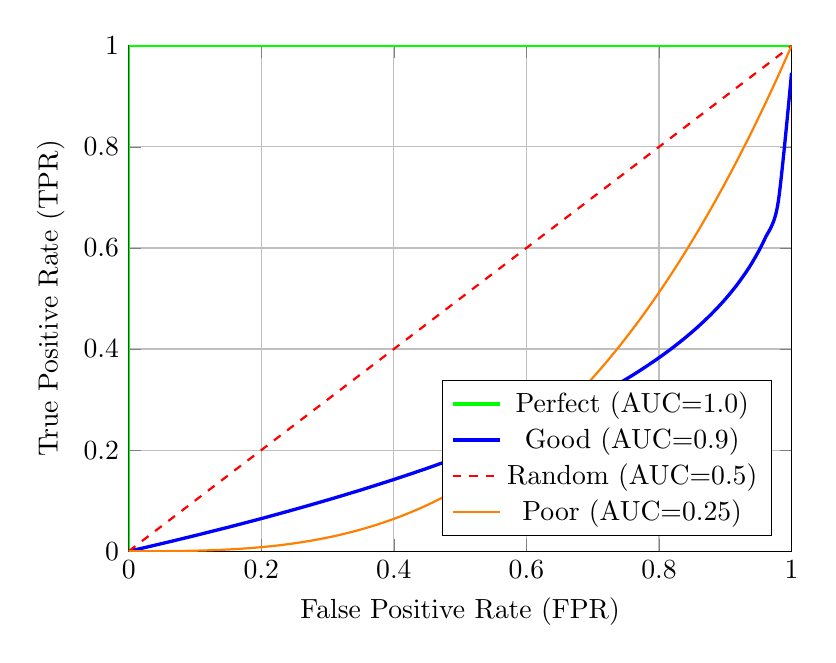
\begin{tikzpicture}
\begin{axis}[
    width=10cm,
    height=8cm,
    xlabel={False Positive Rate (FPR)},
    ylabel={True Positive Rate (TPR)},
    xmin=0, xmax=1,
    ymin=0, ymax=1,
    grid=major,
    legend pos=south east
]
% Perfect classifier
\addplot[green, very thick, domain=0:1] coordinates {(0,0) (0,1) (1,1)};
\addlegendentry{Perfect (AUC=1.0)}

% Good classifier
\addplot[blue, very thick, smooth, domain=0:1, samples=50] {1 - (1-x)^0.3};
\addlegendentry{Good (AUC=0.9)}

% Random classifier
\addplot[red, dashed, thick, domain=0:1] {x};
\addlegendentry{Random (AUC=0.5)}

% Poor classifier
\addplot[orange, thick, smooth, domain=0:1, samples=50] {x^3};
\addlegendentry{Poor (AUC=0.25)}

\end{axis}
\end{tikzpicture}
\caption{ROC curves for different classifier qualities}
\end{figure}

\begin{definition}[AUC (Area Under the Curve)]
\textbf{AUC-ROC} is the area under the ROC curve:
\begin{itemize}
\item AUC = 1.0: Perfect classifier (100\% TPR, 0\% FPR)
\item AUC = 0.5: Random guessing (diagonal line)
\item AUC < 0.5: Worse than random (invert predictions!)
\end{itemize}

\textbf{Interpretation}: Probability that the classifier ranks a random positive example higher than a random negative example.
\end{definition}

\begin{keyidea}
\textbf{Advantages of ROC-AUC}:
\begin{itemize}
\item \textbf{Threshold-independent}: Evaluates all possible thresholds
\item \textbf{Robust to class imbalance}: Unlike accuracy
\item \textbf{Single number summary}: Easy to compare models
\item \textbf{Probabilistic interpretation}: Ranking quality
\end{itemize}

\textbf{When to use ROC vs PR}:
\begin{itemize}
\item \textbf{ROC}: Balanced classes, care about both classes equally
\item \textbf{PR}: Imbalanced classes, focus on positive class (more informative)
\end{itemize}
\end{keyidea}

\subsubsection{Precision-Recall Curve}

\begin{definition}[PR Curve]
Plots Precision vs Recall at various thresholds.

Better for imbalanced datasets where positive class is rare.
\end{definition}

\begin{figure}[H]
\centering
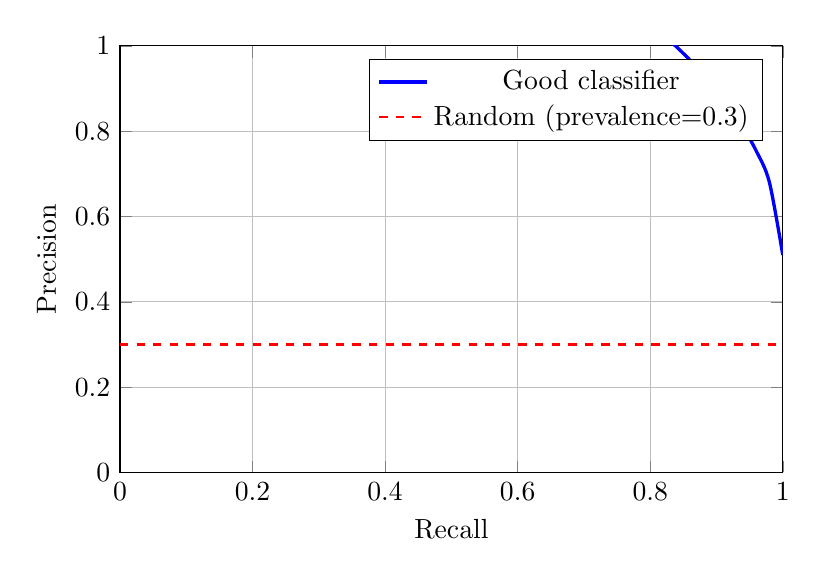
\begin{tikzpicture}
\begin{axis}[
    width=10cm,
    height=7cm,
    xlabel={Recall},
    ylabel={Precision},
    xmin=0, xmax=1,
    ymin=0, ymax=1,
    grid=major,
    legend pos=north east
]
% Good classifier
\addplot[blue, very thick, smooth, domain=0:1, samples=50] {(1-0.1*x)*(1-x^2)^0.5 + 0.5};
\addlegendentry{Good classifier}

% Baseline
\addplot[red, dashed, thick, domain=0:1] {0.3};
\addlegendentry{Random (prevalence=0.3)}

\end{axis}
\end{tikzpicture}
\caption{PR curve: Better classifiers maintain high precision as recall increases}
\end{figure}

\begin{definition}[AP and mAP]
\textbf{Average Precision (AP)}: Area under PR curve (approximation):
\[
AP = \sum_{k=1}^n (R_k - R_{k-1}) P_k
\]
where $P_k$ and $R_k$ are precision and recall at $k$-th threshold.

\textbf{Mean Average Precision (mAP)}: Average AP across multiple classes (used in object detection).
\end{definition}

\subsubsection{Multi-Class Metrics}

\begin{definition}[Multi-Class Extension]
For $K$ classes, confusion matrix is $K \times K$.

\textbf{Macro-averaging}: Compute metric for each class, then average (treats all classes equally).
\[
\text{Macro-F1} = \frac{1}{K}\sum_{k=1}^K F1_k
\]

\textbf{Micro-averaging}: Pool all TP, FP, FN across classes, then compute metric (weights by class size).
\[
\text{Micro-Precision} = \frac{\sum_{k=1}^K TP_k}{\sum_{k=1}^K (TP_k + FP_k)}
\]

\textbf{Weighted-averaging}: Weight each class metric by its support (number of true instances).
\end{definition}

\begin{keyidea}
\textbf{When to use}:
\begin{itemize}
\item \textbf{Macro}: When all classes are equally important (regardless of size)
\item \textbf{Micro}: When larger classes should dominate the metric
\item \textbf{Weighted}: Balance between macro and micro, considering class sizes
\end{itemize}

For imbalanced datasets, macro-averaging can reveal poor performance on minority classes that micro-averaging might hide.
\end{keyidea}

\subsection{Regression Metrics}

\begin{definition}[Regression Metrics]
For predictions $\hat{y}_i$ and true values $y_i$:

\textbf{1. Mean Absolute Error (MAE)}:
\[
MAE = \frac{1}{n}\sum_{i=1}^n |y_i - \hat{y}_i|
\]
Average absolute difference. Robust to outliers, same units as $y$.

\textbf{2. Mean Squared Error (MSE)}:
\[
MSE = \frac{1}{n}\sum_{i=1}^n (y_i - \hat{y}_i)^2
\]
Penalizes large errors heavily. Not in original units.

\textbf{3. Root Mean Squared Error (RMSE)}:
\[
RMSE = \sqrt{MSE} = \sqrt{\frac{1}{n}\sum_{i=1}^n (y_i - \hat{y}_i)^2}
\]
Same scale as $y$. More interpretable than MSE.

\textbf{4. Mean Absolute Percentage Error (MAPE)}:
\[
MAPE = \frac{100\%}{n}\sum_{i=1}^n \left|\frac{y_i - \hat{y}_i}{y_i}\right|
\]
Scale-independent. Undefined when $y_i = 0$.

\textbf{5. R² (Coefficient of Determination)}:
\[
R^2 = 1 - \frac{SS_{\text{res}}}{SS_{\text{tot}}} = 1 - \frac{\sum_i(y_i - \hat{y}_i)^2}{\sum_i(y_i - \bar{y})^2}
\]
where $\bar{y} = \frac{1}{n}\sum_i y_i$.

\begin{itemize}
\item $R^2 = 1$: Perfect predictions
\item $R^2 = 0$: Model no better than predicting mean
\item $R^2 < 0$: Model worse than mean (possible with non-linear models)
\end{itemize}

Measures proportion of variance explained by the model.
\end{definition}

\begin{keyidea}
\textbf{MAE vs MSE/RMSE}:
\begin{itemize}
\item \textbf{MAE}: 
  \begin{itemize}
  \item Robust to outliers
  \item All errors weighted equally
  \item Easier to interpret
  \end{itemize}
\item \textbf{MSE/RMSE}:
  \begin{itemize}
  \item Sensitive to outliers (large errors penalized heavily)
  \item Differentiable everywhere (better for optimization)
  \item Common in statistical theory
  \end{itemize}
\end{itemize}

\textbf{When outliers matter}: Use MAE

\textbf{When large errors are particularly bad}: Use MSE/RMSE

\textbf{R² advantages}:
\begin{itemize}
\item Scale-independent (compare across different problems)
\item Intuitive (percentage of variance explained)
\end{itemize}

\textbf{R² limitations}:
\begin{itemize}
\item Always increases with more features (use adjusted R²)
\item Can be negative for non-linear models
\item Doesn't indicate if model is appropriate
\end{itemize}
\end{keyidea}

% =======================
\section{Model Selection and Hyperparameter Tuning}
% =======================

\subsection{Cross-Validation}

\subsubsection{K-Fold Cross-Validation}

\begin{definition}[K-Fold Cross-Validation]
Split data into $K$ equal-sized folds. For each fold $k$:
\begin{enumerate}
\item Train on folds $\{1, \ldots, K\} \setminus \{k\}$
\item Validate on fold $k$
\item Record validation metric $M_k$
\end{enumerate}
Report average: $\text{CV Score} = \frac{1}{K}\sum_{k=1}^K M_k$

Common: $K = 5$ or $K = 10$.
\end{definition}

\begin{figure}[H]
\centering
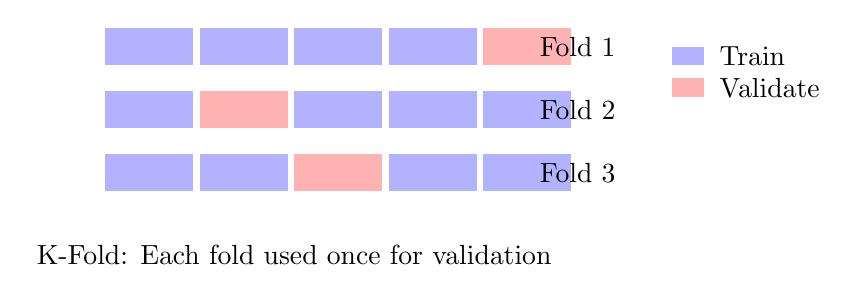
\begin{tikzpicture}[scale=0.8]
% Fold 1
\foreach \i in {0,1,2,3} {
    \fill[blue!30] (\i*1.5, 0) rectangle (\i*1.5+1.4, 0.6);
}
\fill[red!30] (4*1.5, 0) rectangle (4*1.5+1.4, 0.6);
\node at (7.5, 0.3) {Fold 1};

% Fold 2
\foreach \i in {0,2,3,4} {
    \fill[blue!30] (\i*1.5, -1) rectangle (\i*1.5+1.4, -0.4);
}
\fill[red!30] (1*1.5, -1) rectangle (1*1.5+1.4, -0.4);
\node at (7.5, -0.7) {Fold 2};

% Fold 3
\foreach \i in {0,1,3,4} {
    \fill[blue!30] (\i*1.5, -2) rectangle (\i*1.5+1.4, -1.4);
}
\fill[red!30] (2*1.5, -2) rectangle (2*1.5+1.4, -1.4);
\node at (7.5, -1.7) {Fold 3};

% Legend
\fill[blue!30] (9, 0) rectangle (9.5, 0.3);
\node[right] at (9.6, 0.15) {Train};
\fill[red!30] (9, -0.5) rectangle (9.5, -0.2);
\node[right] at (9.6, -0.35) {Validate};

\node at (3, -3) {K-Fold: Each fold used once for validation};
\end{tikzpicture}
\caption{5-fold cross-validation: Each fold serves as validation set once}
\end{figure}

\begin{algorithmbox}
\textbf{K-Fold Cross-Validation}

\textbf{Input}: Data $\mathcal{D}$, model/hyperparameters, $K$

\begin{enumerate}
\item Split $\mathcal{D}$ into $K$ equal-sized folds: $\{\mathcal{D}_1, \ldots, \mathcal{D}_K\}$

\item \textbf{For} $k = 1$ to $K$:
\begin{itemize}
\item $\mathcal{D}_{\text{train}} = \mathcal{D} \setminus \mathcal{D}_k$
\item $\mathcal{D}_{\text{val}} = \mathcal{D}_k$
\item Train model on $\mathcal{D}_{\text{train}}$
\item Evaluate on $\mathcal{D}_{\text{val}}$, record score $M_k$
\end{itemize}

\item Compute average score: $\bar{M} = \frac{1}{K}\sum_{k=1}^K M_k$

\item (Optional) Compute standard deviation: $\sigma_M = \sqrt{\frac{1}{K}\sum_{k=1}^K (M_k - \bar{M})^2}$
\end{enumerate}

\textbf{Output}: Mean score $\bar{M}$ and std $\sigma_M$
\end{algorithmbox}

\begin{keyidea}
\textbf{Why Cross-Validation?}

\textbf{Problem with single train/val split}:
\begin{itemize}
\item High variance (depends on random split)
\item Wastes data (validation set not used for training)
\item May not be representative
\end{itemize}

\textbf{CV advantages}:
\begin{itemize}
\item Lower variance estimate
\item Uses all data for both training and validation
\item Provides confidence interval (via standard deviation)
\item More reliable for model selection
\end{itemize}

\textbf{Choosing $K$}:
\begin{itemize}
\item \textbf{Small $K$ (e.g., 3)}: Faster, higher bias, higher variance
\item \textbf{Large $K$ (e.g., 10)}: Slower, lower bias, can have higher variance
\item \textbf{$K = n$ (LOOCV)}: Maximum data per fold, very slow, high variance
\item \textbf{Common choice}: $K = 5$ or $10$ (good trade-off)
\end{itemize}
\end{keyidea}

\subsubsection{Stratified K-Fold}

\begin{definition}[Stratified K-Fold]
For classification, ensure each fold has approximately the same class distribution as the full dataset.

Particularly important for:
\begin{itemize}
\item Imbalanced datasets
\item Small datasets
\item Multi-class problems
\end{itemize}
\end{definition}

\begin{example}[Stratified Split]
Dataset: 100 examples, 80 class A, 20 class B (80/20 split).

\textbf{Regular 5-fold}: Some folds might have 70/30 or 90/10 (random variation).

\textbf{Stratified 5-fold}: Each fold has exactly 16 class A, 4 class B (80/20 maintained).
\end{example}

\subsubsection{Time Series Cross-Validation}

\begin{definition}[Time Series Split]
For temporal data, cannot randomly shuffle (violates temporal order).

\textbf{Forward chaining}:
\begin{itemize}
\item Fold 1: Train on $[1:n_1]$, validate on $[n_1+1:n_2]$
\item Fold 2: Train on $[1:n_2]$, validate on $[n_2+1:n_3]$
\item Fold 3: Train on $[1:n_3]$, validate on $[n_3+1:n_4]$
\item ...
\end{itemize}

Always train on past, predict future (no data leakage).
\end{definition}

\subsection{Hyperparameter Tuning}

\subsubsection{Grid Search}

\begin{definition}[Grid Search]
Exhaustively search over a specified hyperparameter grid.

\textbf{Example}: For SVM with RBF kernel:
\begin{itemize}
\item $C \in \{0.1, 1, 10, 100\}$
\item $\gamma \in \{0.001, 0.01, 0.1, 1\}$
\end{itemize}
Test all $4 \times 4 = 16$ combinations.
\end{definition}

\begin{algorithmbox}
\textbf{Grid Search with Cross-Validation}

\textbf{Input}: Training data $\mathcal{D}$, model, hyperparameter grid, $K$ for CV

\begin{enumerate}
\item Generate all combinations of hyperparameters from grid

\item \textbf{For} each combination $\theta$:
\begin{itemize}
\item Run $K$-fold CV with hyperparameters $\theta$
\item Record mean CV score $\bar{M}(\theta)$
\end{itemize}

\item Select best: $\theta^* = \argmax_\theta \bar{M}(\theta)$

\item Retrain final model on all data with $\theta^*$
\end{enumerate}

\textbf{Output}: Best hyperparameters $\theta^*$, trained model
\end{algorithmbox}

\begin{keyidea}
\textbf{Grid Search Advantages}:
\begin{itemize}
\item Simple, easy to implement
\item Guaranteed to find best combination in grid
\item Parallelizable (each combination independent)
\item Reproducible
\end{itemize}

\textbf{Limitations}:
\begin{itemize}
\item \textbf{Curse of dimensionality}: $n$ parameters with $k$ values each $\to$ $k^n$ combinations
\item Wastes computation on unpromising regions
\item Grid may miss optimal values between grid points
\item Expensive for large grids or slow models
\end{itemize}

\textbf{Best practices}:
\begin{itemize}
\item Start with coarse grid, then refine around best values
\item Use logarithmic spacing for parameters spanning orders of magnitude
\item Limit grid size (test 3-5 values per parameter max)
\end{itemize}
\end{keyidea}

\subsubsection{Random Search}

\begin{definition}[Random Search]
Sample hyperparameter combinations randomly from specified distributions.

Instead of grid, define distributions:
\begin{itemize}
\item $C \sim \text{LogUniform}(10^{-3}, 10^3)$
\item $\gamma \sim \text{LogUniform}(10^{-4}, 10^1)$
\end{itemize}

Sample $n$ random combinations, evaluate each.
\end{definition}

\begin{theorem}[Random Search Efficiency]
Random search is often more efficient than grid search because:
\begin{itemize}
\item Some hyperparameters matter more than others
\item Random search explores more unique values for important parameters
\item With same budget, covers search space better
\end{itemize}

For $n$ trials:
\begin{itemize}
\item Grid search with 2 parameters: $\sqrt{n} \times \sqrt{n}$ grid
\item Random search: $n$ unique values per parameter
\end{itemize}
\end{theorem}

\begin{figure}[H]
\centering
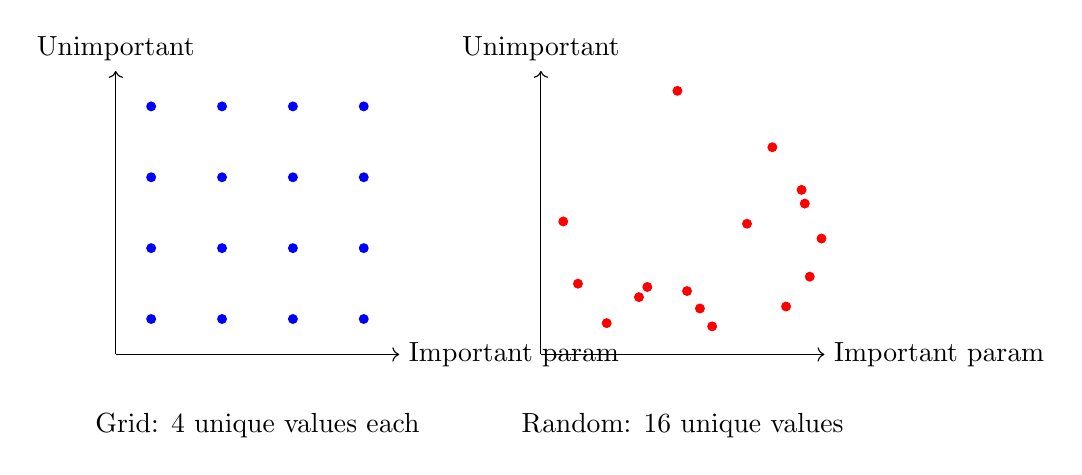
\begin{tikzpicture}[scale=0.9]
% Grid search
\begin{scope}
\draw[->] (0,0) -- (4,0) node[right] {Important param};
\draw[->] (0,0) -- (0,4) node[above] {Unimportant};
\foreach \x in {0.5,1.5,2.5,3.5} {
    \foreach \y in {0.5,1.5,2.5,3.5} {
        \fill[blue] (\x,\y) circle (2pt);
    }
}
\node at (2, -1) {Grid: 4 unique values each};
\end{scope}

% Random search
\begin{scope}[shift={(6,0)}]
\draw[->] (0,0) -- (4,0) node[right] {Important param};
\draw[->] (0,0) -- (0,4) node[above] {Unimportant};
% Random points
\foreach \i in {1,...,16} {
    \pgfmathsetmacro{\x}{rnd*3.8+0.2}
    \pgfmathsetmacro{\y}{rnd*3.8+0.2}
    \fill[red] (\x,\y) circle (2pt);
}
\node at (2, -1) {Random: 16 unique values};
\end{scope}
\end{tikzpicture}
\caption{Grid vs Random search: Random explores more values for important parameter}
\end{figure}

\begin{implementationbox}
\textbf{Random Search in Practice}:

\begin{lstlisting}[language=Python]
from sklearn.model_selection import RandomizedSearchCV
from scipy.stats import loguniform, randint

# Define distributions
param_distributions = {
    'C': loguniform(1e-3, 1e3),
    'gamma': loguniform(1e-4, 1e1),
    'kernel': ['rbf', 'poly']
}

# Random search with 100 iterations
random_search = RandomizedSearchCV(
    estimator=SVC(),
    param_distributions=param_distributions,
    n_iter=100,  # number of random samples
    cv=5,
    random_state=42,
    n_jobs=-1  # parallel
)

random_search.fit(X_train, y_train)
best_params = random_search.best_params_
\end{lstlisting}
\end{implementationbox}

\subsubsection{Bayesian Optimization}

\begin{definition}[Bayesian Optimization]
Intelligent search that uses past evaluations to guide future trials.

\textbf{Key idea}:
\begin{enumerate}
\item Build probabilistic model (surrogate) of $f(\theta)$ where $\theta$ are hyperparameters
\item Use model to select promising $\theta$ (acquisition function)
\item Evaluate $f(\theta)$, update model
\item Repeat
\end{enumerate}

Common surrogate: Gaussian Process (GP)

Common acquisition functions:
\begin{itemize}
\item \textbf{Expected Improvement (EI)}: Balance exploration/exploitation
\item \textbf{Upper Confidence Bound (UCB)}: $\mu(\theta) + \kappa\sigma(\theta)$
\end{itemize}
\end{definition}

\begin{keyidea}
\textbf{Bayesian Optimization vs Random/Grid}:

\textbf{Advantages}:
\begin{itemize}
\item Much more sample-efficient (fewer evaluations needed)
\item Learns from past trials
\item Handles expensive black-box functions well
\item Can incorporate prior knowledge
\end{itemize}

\textbf{Disadvantages}:
\begin{itemize}
\item More complex to implement
\item Overhead in building surrogate model
\item Less parallelizable
\item Can get stuck in local optima
\end{itemize}

\textbf{When to use}:
\begin{itemize}
\item Expensive evaluations (training takes hours)
\item Limited budget (can only try 10-50 configurations)
\item Continuous hyperparameters
\item Black-box optimization
\end{itemize}

\textbf{Popular libraries}: Optuna, Hyperopt, Scikit-Optimize, Ray Tune
\end{keyidea}

\subsection{Nested Cross-Validation}

\begin{definition}[Nested CV]
For unbiased performance estimation with hyperparameter tuning:

\textbf{Outer loop} (performance estimation):
\begin{itemize}
\item $K_{\text{outer}}$-fold CV
\end{itemize}

\textbf{Inner loop} (hyperparameter selection):
\begin{itemize}
\item For each outer fold, run $K_{\text{inner}}$-fold CV on training portion
\item Select best hyperparameters
\item Evaluate on outer fold's validation set
\end{itemize}

This prevents optimistic bias from tuning on the same data used for evaluation.
\end{definition}

\begin{figure}[H]
\centering
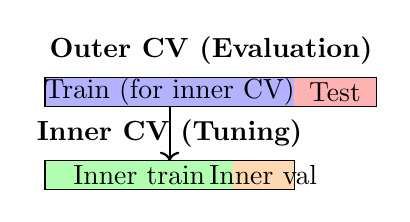
\begin{tikzpicture}[scale=0.7]
\node at (3, 3) {\textbf{Outer CV (Evaluation)}};
\draw[thick] (0, 2.5) rectangle (6, 2);
\fill[blue!30] (0, 2.5) rectangle (4.5, 2);
\fill[red!30] (4.5, 2.5) rectangle (6, 2);
\node at (2.25, 2.25) {Train (for inner CV)};
\node at (5.25, 2.25) {Test};

\node at (2.25, 1.5) {\textbf{Inner CV (Tuning)}};
\draw[thick] (0, 1) rectangle (4.5, 0.5);
\fill[green!30] (0, 1) rectangle (3.4, 0.5);
\fill[orange!30] (3.4, 1) rectangle (4.5, 0.5);
\node at (1.7, 0.75) {Inner train};
\node at (3.95, 0.75) {Inner val};

\draw[->, thick] (2.25, 2) -- (2.25, 1);
\end{tikzpicture}
\caption{Nested CV: Inner loop tunes hyperparameters, outer loop evaluates performance}
\end{figure}

% =======================
\section{Data Preprocessing}
% =======================

\subsection{Feature Scaling}

\subsubsection{Standardization (Z-score Normalization)}

\begin{definition}[Standardization]
Transform features to have mean 0 and standard deviation 1:
\[
x_{\text{scaled}} = \frac{x - \mu}{\sigma}
\]
where $\mu = \frac{1}{n}\sum_i x_i$ and $\sigma = \sqrt{\frac{1}{n}\sum_i (x_i - \mu)^2}$.

Result: $x_{\text{scaled}} \sim \mathcal{N}(0, 1)$ if original data is Gaussian.
\end{definition}

\begin{definition}[Min-Max Normalization]
Scale features to a fixed range, typically $[0, 1]$:
\[
x_{\text{scaled}} = \frac{x - x_{\min}}{x_{\max} - x_{\min}}
\]

For range $[a, b]$:
\[
x_{\text{scaled}} = a + (b - a) \cdot \frac{x - x_{\min}}{x_{\max} - x_{\min}}
\]
\end{definition}

\begin{keyidea}
\textbf{When to use which}:

\textbf{Standardization}:
\begin{itemize}
\item Features have different units/scales
\item Many ML algorithms (SVM, logistic regression, neural networks)
\item When outliers should not be emphasized
\item Preserves outlier information (can go beyond $[0,1]$)
\end{itemize}

\textbf{Min-Max}:
\begin{itemize}
\item Need bounded range (e.g., $[0,1]$)
\item Neural networks (especially with bounded activations like sigmoid)
\item Image data (pixel values)
\item When you want to preserve zero values
\end{itemize}

\textbf{When NOT to scale}:
\begin{itemize}
\item Tree-based models (decision trees, random forests, XGBoost)---invariant to monotonic transformations
\item Features already on same scale
\item Interpretability matters (keep original units)
\end{itemize}
\end{keyidea}

\begin{implementationbox}
\textbf{Critical: Fit on Training, Transform on Test}

\begin{lstlisting}[language=Python]
from sklearn.preprocessing import StandardScaler

# Correct way
scaler = StandardScaler()
X_train_scaled = scaler.fit_transform(X_train)
X_test_scaled = scaler.transform(X_test)  # Use training statistics

# Wrong way (data leakage!)
# scaler.fit(X_test)  # Never fit on test data!
\end{lstlisting}

\textbf{Why?} Test data should be completely unseen. Using test statistics would leak information.
\end{implementationbox}

\subsection{Encoding Categorical Variables}

\subsubsection{Label Encoding}

\begin{definition}[Label Encoding]
Map categories to integers:
\[
\text{Red} \to 0, \quad \text{Green} \to 1, \quad \text{Blue} \to 2
\]

\textbf{Issue}: Introduces artificial ordering ($\text{Blue} > \text{Green} > \text{Red}$).

\textbf{When to use}:
\begin{itemize}
\item Ordinal variables (Low $<$ Medium $<$ High)
\item Tree-based models (can split on integers)
\item Target variable in classification
\end{itemize}
\end{definition}

\subsubsection{One-Hot Encoding}

\begin{definition}[One-Hot Encoding]
Create binary column for each category:

\begin{center}
\begin{tabular}{c|ccc}
Original & Red & Green & Blue \\
\hline
Red & 1 & 0 & 0 \\
Green & 0 & 1 & 0 \\
Blue & 0 & 0 & 1 \\
\end{tabular}
\end{center}

For $K$ categories, creates $K$ binary features (or $K-1$ to avoid multicollinearity).
\end{definition}

\begin{keyidea}
\textbf{One-Hot Advantages}:
\begin{itemize}
\item No artificial ordering
\item Works with linear models
\item Standard approach for neural networks
\end{itemize}

\textbf{Limitations}:
\begin{itemize}
\item \textbf{High cardinality}: Many categories $\to$ many features
\item \textbf{Sparse matrices}: Most values are 0
\item \textbf{Curse of dimensionality}: $K$ categories = $K$ new dimensions
\end{itemize}

\textbf{Alternatives for high cardinality}:
\begin{itemize}
\item \textbf{Target encoding}: Replace category with mean target value
\item \textbf{Frequency encoding}: Replace with category frequency
\item \textbf{Embedding layers}: Neural network learns dense representations (NLP, RecSys)
\item \textbf{Hashing trick}: Hash categories to fixed number of buckets
\end{itemize}
\end{keyidea}

\subsection{Handling Missing Data}

\begin{definition}[Types of Missingness]

\textbf{1. MCAR (Missing Completely At Random)}:
\begin{itemize}
\item Missingness independent of observed and unobserved data
\item Example: Survey responses lost due to server crash
\end{itemize}

\textbf{2. MAR (Missing At Random)}:
\begin{itemize}
\item Missingness depends on observed data, not unobserved
\item Example: Older people less likely to report income (age is observed)
\end{itemize}

\textbf{3. MNAR (Missing Not At Random)}:
\begin{itemize}
\item Missingness depends on unobserved data
\item Example: High earners don't report income (income itself causes missingness)
\end{itemize}
\end{definition}

\begin{definition}[Handling Strategies]

\textbf{1. Deletion}:
\begin{itemize}
\item \textbf{Listwise}: Remove entire row if any feature missing
\item \textbf{Pairwise}: Use available data for each analysis
\item \textbf{When}: MCAR, small amount of missing data ($<$ 5\%)
\end{itemize}

\textbf{2. Imputation}:
\begin{itemize}
\item \textbf{Mean/Median/Mode}: Simple, fast, but ignores relationships
\item \textbf{Forward/Backward fill}: For time series
\item \textbf{KNN imputation}: Use $k$ nearest neighbors' values
\item \textbf{Model-based}: Regression, EM algorithm, MICE
\item \textbf{Indicator variable}: Add binary flag for missingness (preserves information)
\end{itemize}

\textbf{3. Model-Specific}:
\begin{itemize}
\item Some algorithms handle missing values natively (XGBoost, LightGBM)
\end{itemize}
\end{definition}

\begin{implementationbox}
\textbf{Imputation Best Practices}:

\begin{lstlisting}[language=Python]
from sklearn.impute import SimpleImputer, KNNImputer

# Simple imputation
imputer = SimpleImputer(strategy='mean')  # or 'median', 'most_frequent'
X_train_imputed = imputer.fit_transform(X_train)
X_test_imputed = imputer.transform(X_test)

# KNN imputation (more sophisticated)
knn_imputer = KNNImputer(n_neighbors=5)
X_train_imputed = knn_imputer.fit_transform(X_train)
\end{lstlisting}

\textbf{Remember}: Always fit imputer on training data only!
\end{implementationbox}

\subsection{Outlier Detection and Treatment}

\begin{definition}[Outlier Detection Methods]

\textbf{1. Statistical}:
\begin{itemize}
\item \textbf{Z-score}: $|z| > 3$ (assuming Gaussian)
\item \textbf{IQR method}: Below $Q_1 - 1.5 \cdot IQR$ or above $Q_3 + 1.5 \cdot IQR$
\end{itemize}

\textbf{2. Distance-based}:
\begin{itemize}
\item \textbf{DBSCAN}: Points marked as noise
\item \textbf{KNN}: Points with large distance to $k$-th neighbor
\end{itemize}

\textbf{3. Model-based}:
\begin{itemize}
\item \textbf{Isolation Forest}: Isolates outliers in random trees
\item \textbf{One-Class SVM}: Learns boundary around normal data
\item \textbf{Local Outlier Factor (LOF)}: Compares local density
\end{itemize}
\end{definition}

\begin{keyidea}
\textbf{Handling Outliers}:

\textbf{1. Investigate first}:
\begin{itemize}
\item Data error (typo, measurement error)? → Correct or remove
\item Valid extreme value? → Keep (important information)
\end{itemize}

\textbf{2. Treatment options}:
\begin{itemize}
\item \textbf{Keep}: If valid and informative
\item \textbf{Remove}: If errors or not representative
\item \textbf{Cap/Winsorize}: Replace with threshold (e.g., 95th percentile)
\item \textbf{Transform}: Log, square root to reduce impact
\item \textbf{Separate model}: Build model specifically for outliers
\end{itemize}

\textbf{3. Model robustness}:
\begin{itemize}
\item \textbf{Robust models}: Tree-based methods, robust regression (Huber loss)
\item \textbf{Sensitive models}: Linear regression, KNN, SVM (need preprocessing)
\end{itemize}
\end{keyidea}

% =======================
\section{Feature Engineering}
% =======================

\subsection{Feature Extraction vs Selection}

\begin{definition}[Feature Engineering]

\textbf{Feature Extraction}: Create new features from existing ones
\begin{itemize}
\item PCA: Linear combinations
\item Polynomial features: $x_1 \cdot x_2$, $x_1^2$
\item Domain-specific transformations
\end{itemize}

\textbf{Feature Selection}: Choose subset of existing features
\begin{itemize}
\item Remove irrelevant or redundant features
\item Improve model performance and interpretability
\item Reduce overfitting and training time
\end{itemize}
\end{definition}

\subsection{Feature Selection Methods}

\subsubsection{Filter Methods}

\begin{definition}[Filter Methods]
Select features based on statistical measures, independent of model.

\textbf{1. Correlation}:
Remove features highly correlated with each other (redundant).

\textbf{2. Mutual Information}:
\[
MI(X, Y) = \sum_{x,y} P(x,y) \log\frac{P(x,y)}{P(x)P(y)}
\]
Measures dependence between feature and target (captures non-linear relationships).

\textbf{3. Chi-Square Test}:
For categorical features and classification:
\[
\chi^2 = \sum_{i,j} \frac{(O_{ij} - E_{ij})^2}{E_{ij}}
\]
Tests independence between feature and target.

\textbf{4. ANOVA F-test}:
For continuous features and categorical target. Tests if feature means differ across classes.
\end{definition}

\begin{keyidea}
\textbf{Filter Methods}:

\textbf{Advantages}:
\begin{itemize}
\item Fast (no model training)
\item Model-agnostic
\item Good for preprocessing
\end{itemize}

\textbf{Limitations}:
\begin{itemize}
\item Ignores feature interactions
\item Doesn't consider model performance
\item May select redundant features
\end{itemize}
\end{keyidea}

\subsubsection{Wrapper Methods}

\begin{definition}[Wrapper Methods]
Use model performance to guide feature selection.

\textbf{1. Forward Selection}:
\begin{enumerate}
\item Start with no features
\item Add one feature at a time (choose best improvement)
\item Stop when no improvement
\end{enumerate}

\textbf{2. Backward Elimination}:
\begin{enumerate}
\item Start with all features
\item Remove one feature at a time (remove worst)
\item Stop when removal hurts performance
\end{enumerate}

\textbf{3. Recursive Feature Elimination (RFE)}:
\begin{enumerate}
\item Train model on all features
\item Rank features by importance
\item Remove least important
\item Repeat until desired number of features
\end{enumerate}
\end{definition}

\begin{algorithmbox}
\textbf{Recursive Feature Elimination (RFE)}

\textbf{Input}: Features $\vect{X}$, target $\vect{y}$, model, target feature count $k$

\textbf{Initialize}: Current feature set $\mathcal{F} = \{\text{all features}\}$

\textbf{While} $|\mathcal{F}| > k$:
\begin{enumerate}
\item Train model on features in $\mathcal{F}$
\item Compute feature importances (e.g., coefficients, Gini importance)
\item Remove feature with lowest importance from $\mathcal{F}$
\end{enumerate}

\textbf{Output}: Selected features $\mathcal{F}$
\end{algorithmbox}

\begin{keyidea}
\textbf{Wrapper Methods}:

\textbf{Advantages}:
\begin{itemize}
\item Considers model performance directly
\item Can capture feature interactions
\item Optimizes for specific model
\end{itemize}

\textbf{Limitations}:
\begin{itemize}
\item Computationally expensive (many model trainings)
\item Risk of overfitting (especially with small data)
\item Model-specific (selected features may not work for other models)
\end{itemize}
\end{keyidea}

\subsubsection{Embedded Methods}

\begin{definition}[Embedded Methods]
Feature selection built into model training.

\textbf{1. L1 Regularization (Lasso)}:
Penalty $\lambda\sum_j |w_j|$ drives some weights to exactly zero.

\textbf{2. Tree-based Feature Importance}:
Random Forest, XGBoost provide importance scores. Select top $k$ features.

\textbf{3. ElasticNet}:
Combines L1 (sparsity) and L2 (grouping) penalties.
\end{definition}

\begin{keyidea}
\textbf{Embedded Methods}:

\textbf{Advantages}:
\begin{itemize}
\item Faster than wrapper methods
\item Less overfitting risk
\item Integrated with training
\end{itemize}

\textbf{Best Practice}:
\begin{enumerate}
\item Start with filter methods (fast preprocessing)
\item Use embedded methods if model supports (L1, tree importance)
\item Use wrapper methods for critical applications with budget
\end{enumerate}
\end{keyidea}

\subsection{Domain-Specific Feature Engineering}

\begin{example}[Common Transformations]

\textbf{1. Time Features} (from datetime):
\begin{itemize}
\item Hour, day of week, month, year
\item Is weekend? Is holiday?
\item Time since event
\item Cyclic encoding: $\sin(2\pi \cdot \text{hour}/24)$, $\cos(2\pi \cdot \text{hour}/24)$
\end{itemize}

\textbf{2. Text Features}:
\begin{itemize}
\item Bag of words, TF-IDF
\item N-grams
\item Length, number of words, capitals
\item Sentiment scores
\item Word embeddings (Word2Vec, GloVe)
\end{itemize}

\textbf{3. Geospatial}:
\begin{itemize}
\item Distance to landmark
\item Cluster of locations
\item Urban vs rural classification
\end{itemize}

\textbf{4. Interaction Features}:
\begin{itemize}
\item Products: $x_1 \cdot x_2$
\item Ratios: $x_1 / x_2$
\item Differences: $x_1 - x_2$
\end{itemize}

\textbf{5. Aggregations} (for grouped data):
\begin{itemize}
\item Mean, median, std per group
\item Count, min, max per group
\item Time-based: rolling averages, lag features
\end{itemize}
\end{example}

\subsection{Summary of Part 6}

\begin{tcolorbox}[colback=yellow!10!white,colframe=orange!75!black,title=Key Takeaways]
\begin{enumerate}
\item \textbf{Classification Metrics}: Confusion matrix, precision, recall, F1. ROC-AUC for balanced data, PR curve for imbalanced. Choose metric based on cost of errors.

\item \textbf{Regression Metrics}: MAE (robust to outliers), RMSE (penalizes large errors), R² (variance explained). Choose based on error characteristics.

\item \textbf{Cross-Validation}: K-fold for robust evaluation. Stratified for classification. Time series split for temporal data. Nested CV for hyperparameter tuning.

\item \textbf{Hyperparameter Tuning}: Grid search (exhaustive), random search (efficient), Bayesian optimization (sample-efficient for expensive evaluations).

\item \textbf{Feature Scaling}: Standardization (most ML algorithms), Min-Max (bounded activations). Always fit on training, transform on test.

\item \textbf{Categorical Encoding}: Label for ordinal, one-hot for nominal. Target encoding for high cardinality.

\item \textbf{Missing Data}: Understand missingness type (MCAR/MAR/MNAR). Imputation strategies from simple (mean) to complex (KNN, model-based).

\item \textbf{Feature Selection}: Filter (fast, model-agnostic), wrapper (model-specific, expensive), embedded (integrated). Use based on computational budget and goals.
\end{enumerate}

\textbf{Next Steps}: Part 7 covers practical tools and deployment: WEKA, scikit-learn pipelines, and model serving strategies.
\end{tcolorbox}

\begin{exercise}
\begin{enumerate}
\item Given confusion matrix with TP=85, TN=40, FP=10, FN=15, compute accuracy, precision, recall, F1, and specificity.

\item Explain why accuracy is misleading for a dataset with 95\% negative class, 5\% positive class. What metrics would you use instead?

\item For a cancer detection model, would you prioritize precision or recall? Justify your answer and suggest an appropriate threshold strategy.

\item Implement 5-fold cross-validation by hand for a dataset with 100 examples. Show which examples go in which fold.

\item Why must we fit the scaler on training data only? What happens if we fit on all data (train + test)?

\item Design one-hot encoding for categorical variable \{Red, Green, Blue, Red, Green\}. How many columns? Should you use $K$ or $K-1$ columns?

\item Compare computational complexity: Grid search with 4 parameters (5 values each) vs random search with 100 iterations. Which tries more unique combinations for each parameter?

\item For time series data, why can't we use regular k-fold cross-validation? Design a proper time series CV scheme for 120 monthly observations.
\end{enumerate}
\end{exercise}

% =======================
% Part 7: Tools, Pipelines, and Deployment
% =======================
\addcontentsline{toc}{section}{Part 7: Tools, Pipelines, and Deployment}
\section*{Part 7: Tools, Pipelines, and Deployment}

\section{WEKA: Practical Guide}

\subsection{Introduction to WEKA}

\begin{definition}[WEKA]
\textbf{WEKA (Waikato Environment for Knowledge Analysis)} is a collection of machine learning algorithms for data mining tasks. Developed at University of Waikato, New Zealand.

\textbf{Key Features}:
\begin{itemize}
\item GUI-based interface (no coding required)
\item Extensive algorithm library (classification, regression, clustering, etc.)
\item Built-in visualization tools
\item Java-based (cross-platform)
\item Free and open-source
\end{itemize}

\textbf{When to use WEKA}:
\begin{itemize}
\item Quick prototyping and experimentation
\item Teaching and learning ML concepts
\item Comparing multiple algorithms easily
\item Small to medium datasets
\item When GUI is preferred over coding
\end{itemize}
\end{definition}

\subsection{WEKA Explorer Interface}

\begin{keyidea}
\textbf{WEKA Explorer has 6 main tabs}:

\textbf{1. Preprocess}: Load data, view statistics, apply filters
\begin{itemize}
\item Import ARFF, CSV, JDBC databases
\item View attribute statistics and distributions
\item Apply filters (discretization, normalization, attribute selection)
\end{itemize}

\textbf{2. Classify}: Train classification/regression models
\begin{itemize}
\item Choose algorithm from tree structure
\item Configure hyperparameters
\item Select test options (cross-validation, percentage split, etc.)
\item View results: accuracy, confusion matrix, ROC
\end{itemize}

\textbf{3. Cluster}: Perform clustering
\begin{itemize}
\item K-means, EM, DBSCAN, hierarchical
\item Evaluate clusters
\item Visualize assignments
\end{itemize}

\textbf{4. Associate}: Find association rules
\begin{itemize}
\item Apriori, FP-Growth
\item Set minimum support and confidence
\end{itemize}

\textbf{5. Select attributes}: Feature selection
\begin{itemize}
\item Various search and evaluation methods
\item Rank features by importance
\end{itemize}

\textbf{6. Visualize}: Data exploration
\begin{itemize}
\item Scatter plots, histograms
\item Class distributions
\item Interactive exploration
\end{itemize}
\end{keyidea}

\subsection{Data Format: ARFF}

\begin{definition}[ARFF Format]
ARFF (Attribute-Relation File Format) is WEKA's native format.

\textbf{Structure}:
\begin{lstlisting}
@relation weather

@attribute outlook {sunny, overcast, rainy}
@attribute temperature numeric
@attribute humidity numeric
@attribute windy {TRUE, FALSE}
@attribute play {yes, no}

@data
sunny,85,85,FALSE,no
sunny,80,90,TRUE,no
overcast,83,86,FALSE,yes
rainy,70,96,FALSE,yes
...
\end{lstlisting}

\textbf{Components}:
\begin{itemize}
\item \texttt{@relation}: Dataset name
\item \texttt{@attribute}: Feature name and type (numeric, nominal, string, date)
\item \texttt{@data}: Actual data rows
\end{itemize}
\end{definition}

\subsection{Workflow Example: Classification}

\begin{algorithmbox}
\textbf{WEKA Classification Workflow}

\textbf{Step 1: Load Data}
\begin{itemize}
\item Open Explorer $\to$ Preprocess tab
\item Click ``Open file...'' $\to$ Select ARFF or CSV
\item Review attributes in the table
\item Check class distribution (click on class attribute)
\end{itemize}

\textbf{Step 2: Preprocess (Optional)}
\begin{itemize}
\item Apply filters: Click ``Choose'' under Filter
\item Example: \texttt{unsupervised.attribute.Normalize} for scaling
\item Click ``Apply'' to execute filter
\end{itemize}

\textbf{Step 3: Select Algorithm}
\begin{itemize}
\item Click ``Classify'' tab
\item Click ``Choose'' button
\item Navigate tree: e.g., \texttt{trees $\to$ J48} (decision tree)
\item Click on algorithm name to configure parameters
\end{itemize}

\textbf{Step 4: Choose Test Method}
\begin{itemize}
\item \textbf{Cross-validation}: Select folds (default 10)
\item \textbf{Percentage split}: e.g., 66\% train, 34\% test
\item \textbf{Use training set}: Evaluate on training (overfitting check)
\item \textbf{Supplied test set}: Load separate test file
\end{itemize}

\textbf{Step 5: Run and Evaluate}
\begin{itemize}
\item Click ``Start'' button
\item View results in output area:
\begin{itemize}
\item Summary statistics
\item Confusion matrix
\item Detailed accuracy by class
\end{itemize}
\item Right-click on result $\to$ Visualize for plots
\end{itemize}

\textbf{Step 6: Compare Models}
\begin{itemize}
\item Run multiple algorithms (results stack in result list)
\item Right-click result list $\to$ Compare to compare
\item Export results: Right-click $\to$ Save result buffer
\end{itemize}
\end{algorithmbox}

\subsection{Common WEKA Algorithms}

\begin{table}[H]
\centering
\begin{tabular}{@{}ll@{}}
\toprule
\textbf{Category} & \textbf{Algorithms in WEKA} \\
\midrule
\textbf{Trees} & J48 (C4.5), RandomForest, REPTree \\
\textbf{Rules} & JRip, PART, DecisionTable \\
\textbf{Functions} & Logistic, MultilayerPerceptron, SMO (SVM) \\
\textbf{Lazy} & IBk (KNN), LWL \\
\textbf{Bayes} & NaiveBayes, BayesNet \\
\textbf{Meta} & AdaBoostM1, Bagging, Stacking, Vote \\
\textbf{Clustering} & SimpleKMeans, EM, DBSCAN, HierarchicalClusterer \\
\bottomrule
\end{tabular}
\caption{Common algorithms in WEKA by category}
\end{table}

\subsection{Visualizing Results}

\begin{keyidea}
\textbf{WEKA Visualization Tools}:

\textbf{1. ROC Curve}:
\begin{itemize}
\item After classification: Right-click result $\to$ Visualize threshold curve
\item Choose class and metric (TPR vs FPR for ROC)
\item Compare multiple classifiers on same plot
\end{itemize}

\textbf{2. Classification Errors}:
\begin{itemize}
\item Right-click result $\to$ Visualize classifier errors
\item Shows 2D plot of predictions
\item Misclassified instances highlighted
\item Interactive: hover for details
\end{itemize}

\textbf{3. Tree Visualization}:
\begin{itemize}
\item After training tree (J48, RandomForest): Right-click $\to$ Visualize tree
\item Shows decision rules graphically
\item Can save as PNG/PDF
\end{itemize}

\textbf{4. Cost/Benefit Analysis}:
\begin{itemize}
\item Define cost matrix for different types of errors
\item WEKA computes expected cost
\item Useful for imbalanced datasets
\end{itemize}
\end{keyidea}

\subsection{Advantages and Limitations}

\begin{keyidea}
\textbf{WEKA Advantages}:
\begin{itemize}
\item \textbf{Easy to use}: GUI-based, no programming required
\item \textbf{Comprehensive}: 100+ algorithms built-in
\item \textbf{Educational}: Excellent for learning ML
\item \textbf{Visualization}: Good built-in plots
\item \textbf{Reproducible}: Can save configurations
\end{itemize}

\textbf{WEKA Limitations}:
\begin{itemize}
\item \textbf{Not for production}: GUI-based, not suitable for deployment
\item \textbf{Scalability}: Limited to datasets that fit in memory
\item \textbf{Modern algorithms}: Lacks latest methods (no XGBoost, deep learning)
\item \textbf{Automation}: Difficult to automate workflows
\item \textbf{Customization}: Limited compared to programming libraries
\end{itemize}

\textbf{Best Use Cases}:
\begin{itemize}
\item Academic research and teaching
\item Quick baseline comparisons
\item Data exploration
\item Proof of concept
\end{itemize}

\textbf{When to move beyond WEKA}:
\begin{itemize}
\item Large-scale datasets ($>$1M rows)
\item Production deployment
\item Need for latest algorithms
\item Complex preprocessing pipelines
\item Integration with other systems
\end{itemize}
\end{keyidea}

% =======================
\section{ML Pipelines in Python}
% =======================

\subsection{Introduction to Scikit-learn}

\begin{definition}[Scikit-learn]
Scikit-learn is Python's premier machine learning library, offering:
\begin{itemize}
\item Consistent API across algorithms
\item Comprehensive algorithm coverage
\item Excellent documentation
\item Integration with NumPy, Pandas, Matplotlib
\item Production-ready code
\end{itemize}

\textbf{Core API}: All estimators follow the same pattern:
\begin{lstlisting}[language=Python]
model = Estimator()          # Initialize
model.fit(X_train, y_train)  # Train
predictions = model.predict(X_test)  # Predict
score = model.score(X_test, y_test)  # Evaluate
\end{lstlisting}
\end{definition}

\subsection{The Pipeline Concept}

\begin{definition}[Pipeline]
A \textbf{Pipeline} chains multiple processing steps into a single estimator:
\[
\text{Data} \xrightarrow{\text{Transform 1}} \xrightarrow{\text{Transform 2}} \xrightarrow{\cdots} \xrightarrow{\text{Model}}
\]

\textbf{Benefits}:
\begin{itemize}
\item \textbf{Convenience}: Single \texttt{fit()}/\texttt{predict()} call
\item \textbf{Prevents leakage}: Transformers fit only on training data
\item \textbf{Hyperparameter tuning}: Tune entire pipeline with GridSearchCV
\item \textbf{Reproducibility}: Easy to save and load entire workflow
\item \textbf{Code cleanliness}: Organized preprocessing + modeling
\end{itemize}
\end{definition}

\begin{figure}[H]
\centering
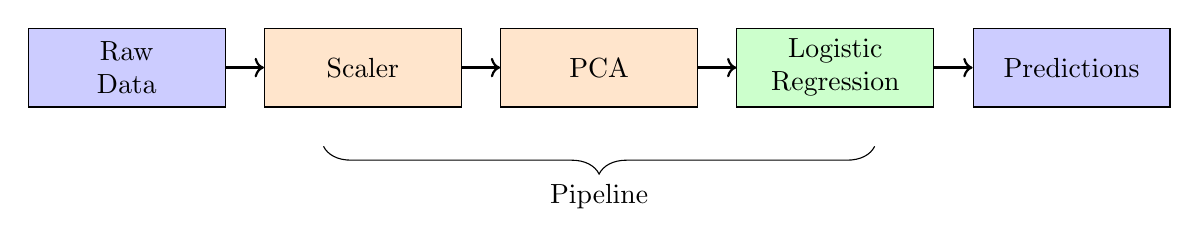
\begin{tikzpicture}[
    box/.style={rectangle, draw, minimum width=25mm, minimum height=10mm, align=center},
    data/.style={fill=blue!20},
    transform/.style={fill=orange!20},
    model/.style={fill=green!20}
]
\node[box, data] (data) at (0,0) {Raw\\Data};
\node[box, transform] (scale) at (3,0) {Scaler};
\node[box, transform] (pca) at (6,0) {PCA};
\node[box, model] (lr) at (9,0) {Logistic\\Regression};
\node[box, data] (pred) at (12,0) {Predictions};

\draw[->, thick] (data) -- (scale);
\draw[->, thick] (scale) -- (pca);
\draw[->, thick] (pca) -- (lr);
\draw[->, thick] (lr) -- (pred);

\draw[decorate, decoration={brace, amplitude=10pt, mirror}] 
    (2.5,-1) -- (9.5,-1) node[midway, below, yshift=-10pt] {Pipeline};
\end{tikzpicture}
\caption{Pipeline chains preprocessing and modeling steps}
\end{figure}

\subsection{Building Pipelines}

\begin{implementationbox}
\textbf{Basic Pipeline Example}:

\begin{lstlisting}[language=Python]
from sklearn.pipeline import Pipeline
from sklearn.preprocessing import StandardScaler
from sklearn.decomposition import PCA
from sklearn.linear_model import LogisticRegression

# Create pipeline
pipeline = Pipeline([
    ('scaler', StandardScaler()),      # Step 1: Scale
    ('pca', PCA(n_components=10)),     # Step 2: Reduce dim
    ('classifier', LogisticRegression()) # Step 3: Classify
])

# Use like any other estimator
pipeline.fit(X_train, y_train)
predictions = pipeline.predict(X_test)
accuracy = pipeline.score(X_test, y_test)

print(f"Accuracy: {accuracy:.3f}")
\end{lstlisting}

\textbf{Key Points}:
\begin{itemize}
\item Each step is a tuple: \texttt{('name', transformer)}
\item All steps except last must have \texttt{fit\_transform()}
\item Last step must have \texttt{fit()} and \texttt{predict()}
\item Access steps: \texttt{pipeline.named\_steps['scaler']}
\end{itemize}
\end{implementationbox}

\subsection{Column Transformer}

\begin{definition}[ColumnTransformer]
Apply different transformations to different columns:

\begin{lstlisting}[language=Python]
from sklearn.compose import ColumnTransformer
from sklearn.preprocessing import StandardScaler, OneHotEncoder

# Define transformations for different column types
preprocessor = ColumnTransformer([
    ('num', StandardScaler(), ['age', 'income']),
    ('cat', OneHotEncoder(), ['gender', 'city'])
])

# Use in pipeline
pipeline = Pipeline([
    ('preprocessor', preprocessor),
    ('classifier', RandomForestClassifier())
])
\end{lstlisting}

\textbf{Benefits}:
\begin{itemize}
\item Handle mixed data types (numerical + categorical)
\item Apply appropriate transformation to each feature type
\item Cleaner than manual column splitting
\end{itemize}
\end{definition}

\subsection{Pipeline with GridSearchCV}

\begin{implementationbox}
\textbf{Hyperparameter Tuning with Pipeline}:

\begin{lstlisting}[language=Python]
from sklearn.model_selection import GridSearchCV

# Create pipeline
pipeline = Pipeline([
    ('scaler', StandardScaler()),
    ('classifier', SVC())
])

# Define parameter grid (use double underscore)
param_grid = {
    'classifier__C': [0.1, 1, 10],
    'classifier__gamma': [0.001, 0.01, 0.1],
    'classifier__kernel': ['rbf', 'linear']
}

# Grid search on entire pipeline
grid_search = GridSearchCV(
    pipeline, 
    param_grid, 
    cv=5, 
    scoring='accuracy',
    n_jobs=-1
)

grid_search.fit(X_train, y_train)

print(f"Best params: {grid_search.best_params_}")
print(f"Best CV score: {grid_search.best_score_:.3f}")

# Use best model
best_model = grid_search.best_estimator_
test_score = best_model.score(X_test, y_test)
\end{lstlisting}

\textbf{Naming convention}: Use \texttt{step\_name\_\_parameter\_name} to reference pipeline parameters.
\end{implementationbox}

\subsection{Custom Transformers}

\begin{definition}[Custom Transformer]
Create your own transformer by inheriting from \texttt{BaseEstimator} and \texttt{TransformerMixin}:

\begin{lstlisting}[language=Python]
from sklearn.base import BaseEstimator, TransformerMixin

class LogTransformer(BaseEstimator, TransformerMixin):
    def __init__(self, features):
        self.features = features
    
    def fit(self, X, y=None):
        return self  # Nothing to learn
    
    def transform(self, X):
        X_copy = X.copy()
        X_copy[self.features] = np.log1p(X_copy[self.features])
        return X_copy

# Use in pipeline
pipeline = Pipeline([
    ('log', LogTransformer(['income', 'age'])),
    ('scaler', StandardScaler()),
    ('model', RandomForestRegressor())
])
\end{lstlisting}

\textbf{Requirements}:
\begin{itemize}
\item Implement \texttt{fit()} (even if it just returns \texttt{self})
\item Implement \texttt{transform()}
\item Optionally implement \texttt{fit\_transform()} (inherited from mixin)
\end{itemize}
\end{definition}

\subsection{Model Persistence}

\subsubsection{Saving and Loading Models}

\begin{implementationbox}
\textbf{Method 1: Joblib (Recommended)}:

\begin{lstlisting}[language=Python]
import joblib

# Save model
joblib.dump(pipeline, 'model_pipeline.joblib')

# Load model
loaded_pipeline = joblib.load('model_pipeline.joblib')

# Use loaded model
predictions = loaded_pipeline.predict(X_new)
\end{lstlisting}

\textbf{Method 2: Pickle}:

\begin{lstlisting}[language=Python]
import pickle

# Save
with open('model.pkl', 'wb') as f:
    pickle.dump(pipeline, f)

# Load
with open('model.pkl', 'rb') as f:
    loaded_model = pickle.load(f)
\end{lstlisting}

\textbf{Joblib vs Pickle}:
\begin{itemize}
\item \textbf{Joblib}: Better for large NumPy arrays (efficient compression)
\item \textbf{Pickle}: More general, works with any Python object
\item Both are not cross-version compatible (save scikit-learn version!)
\end{itemize}
\end{implementationbox}

\subsubsection{Versioning and Reproducibility}

\begin{keyidea}
\textbf{Best Practices for Model Persistence}:

\textbf{1. Save Metadata}:
\begin{lstlisting}[language=Python]
import json
from datetime import datetime

metadata = {
    'model_type': 'RandomForestClassifier',
    'sklearn_version': sklearn.__version__,
    'training_date': datetime.now().isoformat(),
    'features': list(X_train.columns),
    'performance': {
        'train_accuracy': train_acc,
        'test_accuracy': test_acc,
        'cv_score': cv_score
    },
    'hyperparameters': grid_search.best_params_
}

with open('model_metadata.json', 'w') as f:
    json.dump(metadata, f, indent=2)
\end{lstlisting}

\textbf{2. Version Control}:
\begin{itemize}
\item Use Git for code
\item Use DVC (Data Version Control) for models and data
\item Tag model versions: \texttt{v1.0.0}, \texttt{v1.1.0}
\end{itemize}

\textbf{3. Environment Management}:
\begin{lstlisting}[language=bash]
# Save environment
pip freeze > requirements.txt

# Or use conda
conda env export > environment.yml
\end{lstlisting}

\textbf{4. Directory Structure}:
\dirtree{%
.1 project/.
.2 models/.
.3 model\_v1.0.0.joblib.
.3 model\_v1.0.0\_metadata.json.
.2 data/.
.3 train.csv.
.3 test.csv.
.2 notebooks/.
.2 src/.
.3 requirements.txt.
}
\end{keyidea}

\subsection{Complete Pipeline Example}

\begin{implementationbox}
\textbf{End-to-End Pipeline with All Features}:

\begin{lstlisting}[language=Python]
from sklearn.pipeline import Pipeline
from sklearn.compose import ColumnTransformer
from sklearn.preprocessing import StandardScaler, OneHotEncoder
from sklearn.impute import SimpleImputer
from sklearn.ensemble import RandomForestClassifier
from sklearn.model_selection import cross_val_score
import pandas as pd
import joblib

# Define column types
numeric_features = ['age', 'income', 'credit_score']
categorical_features = ['gender', 'education', 'employment']

# Numeric pipeline
numeric_transformer = Pipeline([
    ('imputer', SimpleImputer(strategy='median')),
    ('scaler', StandardScaler())
])

# Categorical pipeline
categorical_transformer = Pipeline([
    ('imputer', SimpleImputer(strategy='most_frequent')),
    ('onehot', OneHotEncoder(handle_unknown='ignore'))
])

# Combine with ColumnTransformer
preprocessor = ColumnTransformer([
    ('num', numeric_transformer, numeric_features),
    ('cat', categorical_transformer, categorical_features)
])

# Full pipeline
pipeline = Pipeline([
    ('preprocessor', preprocessor),
    ('classifier', RandomForestClassifier(random_state=42))
])

# Cross-validation
cv_scores = cross_val_score(
    pipeline, X_train, y_train, 
    cv=5, scoring='accuracy'
)
print(f"CV Accuracy: {cv_scores.mean():.3f} (+/- {cv_scores.std():.3f})")

# Train final model
pipeline.fit(X_train, y_train)

# Evaluate
test_score = pipeline.score(X_test, y_test)
print(f"Test Accuracy: {test_score:.3f}")

# Save
joblib.dump(pipeline, 'credit_model_pipeline.joblib')

# Later: Load and predict
loaded_pipeline = joblib.load('credit_model_pipeline.joblib')
new_predictions = loaded_pipeline.predict(X_new)
\end{lstlisting}
\end{implementationbox}

% =======================
\section{Model Deployment}
% =======================

\subsection{Deployment Considerations}

\begin{keyidea}
\textbf{Key Questions Before Deployment}:

\textbf{1. Latency Requirements}:
\begin{itemize}
\item Real-time ($<$ 100ms): Lightweight models, caching
\item Near real-time (seconds): Most models acceptable
\item Batch processing (hours): Any model size
\end{itemize}

\textbf{2. Scale}:
\begin{itemize}
\item Queries per second (QPS)?
\item Peak vs average load?
\item Need for horizontal scaling?
\end{itemize}

\textbf{3. Infrastructure}:
\begin{itemize}
\item Cloud (AWS, GCP, Azure) vs on-premise?
\item Serverless (Lambda) vs containers (Docker) vs VMs?
\item GPU required?
\end{itemize}

\textbf{4. Monitoring}:
\begin{itemize}
\item Performance metrics (latency, throughput)
\item Model metrics (accuracy, drift detection)
\item System metrics (CPU, memory, errors)
\end{itemize}

\textbf{5. Updates}:
\begin{itemize}
\item How often to retrain?
\item Blue-green deployment vs canary?
\item Rollback strategy?
\end{itemize}
\end{keyidea}

\subsection{Model Export Formats}

\subsubsection{ONNX (Open Neural Network Exchange)}

\begin{definition}[ONNX]
ONNX is an open format for representing ML models, enabling interoperability across frameworks.

\textbf{Benefits}:
\begin{itemize}
\item Train in one framework (PyTorch, scikit-learn), deploy in another
\item Optimized inference engines (ONNX Runtime)
\item Hardware acceleration support
\item Language-agnostic (use from Python, C++, Java, etc.)
\end{itemize}

\begin{lstlisting}[language=Python]
# Convert scikit-learn to ONNX
from skl2onnx import convert_sklearn
from skl2onnx.common.data_types import FloatTensorType

# Define input type
initial_type = [('float_input', FloatTensorType([None, n_features]))]

# Convert
onnx_model = convert_sklearn(
    sklearn_model, 
    initial_types=initial_type
)

# Save
with open("model.onnx", "wb") as f:
    f.write(onnx_model.SerializeToString())

# Load and inference with ONNX Runtime
import onnxruntime as rt

sess = rt.InferenceSession("model.onnx")
input_name = sess.get_inputs()[0].name
pred = sess.run(None, {input_name: X_test.astype(np.float32)})
\end{lstlisting}
\end{definition}

\subsubsection{TensorFlow SavedModel}

\begin{definition}[TensorFlow SavedModel]
TensorFlow's universal format for saving models.

\begin{lstlisting}[language=Python]
import tensorflow as tf

# Save
model.save('saved_model/my_model')

# Load
loaded_model = tf.keras.models.load_model('saved_model/my_model')

# Predict
predictions = loaded_model.predict(X_test)
\end{lstlisting}

\textbf{Benefits}:
\begin{itemize}
\item Complete model serialization (architecture + weights + config)
\item TensorFlow Serving integration
\item TensorFlow Lite for mobile/edge
\end{itemize}
\end{definition}

\subsubsection{Format Comparison}

\begin{table}[H]
\centering
\begin{tabular}{@{}llll@{}}
\toprule
\textbf{Format} & \textbf{Framework} & \textbf{Use Case} & \textbf{Pros} \\
\midrule
Pickle/Joblib & Any Python & Python-only & Simple, native \\
ONNX & Cross-framework & Production & Optimized, portable \\
SavedModel & TensorFlow & TF ecosystem & Complete, TF Serving \\
PMML & Traditional ML & Enterprise & Standardized, legacy \\
\bottomrule
\end{tabular}
\caption{Model export format comparison}
\end{table}

\subsection{Serving Models via REST API}

\subsubsection{Flask API}

\begin{implementationbox}
\textbf{Simple Flask API for Model Serving}:

\begin{lstlisting}[language=Python]
from flask import Flask, request, jsonify
import joblib
import numpy as np

# Initialize Flask app
app = Flask(__name__)

# Load model at startup
model = joblib.load('model_pipeline.joblib')

@app.route('/predict', methods=['POST'])
def predict():
    try:
        # Get JSON data
        data = request.get_json()
        
        # Convert to array
        features = np.array(data['features']).reshape(1, -1)
        
        # Predict
        prediction = model.predict(features)
        probability = model.predict_proba(features)
        
        # Return response
        return jsonify({
            'prediction': int(prediction[0]),
            'probability': probability[0].tolist(),
            'status': 'success'
        })
    
    except Exception as e:
        return jsonify({
            'error': str(e),
            'status': 'error'
        }), 400

@app.route('/health', methods=['GET'])
def health():
    return jsonify({'status': 'healthy'})

if __name__ == '__main__':
    app.run(host='0.0.0.0', port=5000)
\end{lstlisting}

\textbf{Test with curl}:
\begin{lstlisting}[language=bash]
curl -X POST http://localhost:5000/predict \
  -H "Content-Type: application/json" \
  -d '{"features": [25, 50000, 700, 1, 2]}'
\end{lstlisting}
\end{implementationbox}

\subsubsection{FastAPI (Modern Alternative)}

\begin{implementationbox}
\textbf{FastAPI for High-Performance Serving}:

\begin{lstlisting}[language=Python]
from fastapi import FastAPI, HTTPException
from pydantic import BaseModel
import joblib
import numpy as np

# Define input schema
class PredictionRequest(BaseModel):
    features: list[float]

class PredictionResponse(BaseModel):
    prediction: int
    probability: list[float]

# Initialize app
app = FastAPI(title="ML Model API")

# Load model
model = joblib.load('model_pipeline.joblib')

@app.post("/predict", response_model=PredictionResponse)
async def predict(request: PredictionRequest):
    try:
        features = np.array(request.features).reshape(1, -1)
        prediction = model.predict(features)
        probability = model.predict_proba(features)
        
        return PredictionResponse(
            prediction=int(prediction[0]),
            probability=probability[0].tolist()
        )
    except Exception as e:
        raise HTTPException(status_code=400, detail=str(e))

@app.get("/health")
async def health():
    return {"status": "healthy"}

# Run with: uvicorn main:app --reload
\end{lstlisting}

\textbf{FastAPI Advantages}:
\begin{itemize}
\item Automatic API documentation (Swagger UI at \texttt{/docs})
\item Type validation with Pydantic
\item Async support (higher throughput)
\item Modern, faster than Flask
\end{itemize}
\end{implementationbox}

\subsection{Containerization with Docker}

\begin{implementationbox}
\textbf{Dockerfile for ML API}:

\begin{lstlisting}
FROM python:3.9-slim

WORKDIR /app

# Copy requirements and install
COPY requirements.txt .
RUN pip install --no-cache-dir -r requirements.txt

# Copy model and code
COPY model_pipeline.joblib .
COPY app.py .

# Expose port
EXPOSE 5000

# Run app
CMD ["python", "app.py"]
\end{lstlisting}

\textbf{Build and Run}:
\begin{lstlisting}[language=bash]
# Build image
docker build -t ml-model-api .

# Run container
docker run -p 5000:5000 ml-model-api

# Test
curl http://localhost:5000/health
\end{lstlisting}

\textbf{Docker Compose for Multi-Service}:
\begin{lstlisting}
version: '3.8'

services:
  api:
    build: .
    ports:
      - "5000:5000"
    environment:
      - MODEL_PATH=/models/model.joblib
    volumes:
      - ./models:/models
  
  redis:
    image: redis:alpine
    ports:
      - "6379:6379"
\end{lstlisting}
\end{implementationbox}

\subsection{Cloud Deployment}

\begin{keyidea}
\textbf{Cloud Deployment Options}:

\textbf{1. Serverless (AWS Lambda, Google Cloud Functions)}:
\begin{itemize}
\item \textbf{Pros}: No server management, auto-scaling, pay per use
\item \textbf{Cons}: Cold starts, limited execution time, limited memory
\item \textbf{Best for}: Low to medium traffic, event-driven, cost-sensitive
\end{itemize}

\textbf{2. Containers (AWS ECS, GKE, Azure Container Instances)}:
\begin{itemize}
\item \textbf{Pros}: Consistent environments, easy scaling, orchestration
\item \textbf{Cons}: More complex setup, need to manage infrastructure
\item \textbf{Best for}: Medium to high traffic, microservices
\end{itemize}

\textbf{3. Managed ML Services}:
\begin{itemize}
\item AWS SageMaker, Google AI Platform, Azure ML
\item \textbf{Pros}: Built-in monitoring, auto-scaling, A/B testing, versioning
\item \textbf{Cons}: Vendor lock-in, can be expensive
\item \textbf{Best for}: Enterprise ML, need full MLOps
\end{itemize}

\textbf{4. Kubernetes}:
\begin{itemize}
\item \textbf{Pros}: Highly scalable, flexible, cloud-agnostic
\item \textbf{Cons}: Steep learning curve, operational overhead
\item \textbf{Best for}: Large scale, multi-model serving, complex workflows
\end{itemize}
\end{keyidea}

\subsection{Model Monitoring}

\begin{definition}[Model Monitoring]
Continuous tracking of model performance and data quality in production.

\textbf{Key Metrics to Monitor}:

\textbf{1. Performance Metrics}:
\begin{itemize}
\item Prediction accuracy/error
\item Latency (p50, p95, p99)
\item Throughput (requests per second)
\end{itemize}

\textbf{2. Data Quality}:
\begin{itemize}
\item Missing values
\item Out-of-range values
\item Data type mismatches
\end{itemize}

\textbf{3. Data Drift}:
\begin{itemize}
\item Feature distribution changes
\item Target distribution changes
\item KL divergence, KS test
\end{itemize}

\textbf{4. Concept Drift}:
\begin{itemize}
\item $P(y|X)$ changes over time
\item Model accuracy degrades
\item Need retraining
\end{itemize}

\textbf{5. System Metrics}:
\begin{itemize}
\item CPU/memory usage
\item Error rates
\item Uptime
\end{itemize}
\end{definition}

\begin{implementationbox}
\textbf{Simple Logging for Monitoring}:

\begin{lstlisting}[language=Python]
import logging
import time
from datetime import datetime

# Setup logging
logging.basicConfig(level=logging.INFO)
logger = logging.getLogger(__name__)

@app.route('/predict', methods=['POST'])
def predict():
    start_time = time.time()
    
    try:
        data = request.get_json()
        features = np.array(data['features']).reshape(1, -1)
        
        # Predict
        prediction = model.predict(features)
        probability = model.predict_proba(features)
        
        # Log prediction
        latency = time.time() - start_time
        logger.info({
            'timestamp': datetime.now().isoformat(),
            'features': features.tolist(),
            'prediction': int(prediction[0]),
            'confidence': float(probability[0].max()),
            'latency_ms': latency * 1000
        })
        
        return jsonify({
            'prediction': int(prediction[0]),
            'probability': probability[0].tolist()
        })
    
    except Exception as e:
        logger.error(f"Prediction error: {str(e)}")
        return jsonify({'error': str(e)}), 400
\end{lstlisting}

\textbf{Advanced}: Use dedicated tools like Prometheus, Grafana, ELK stack, or cloud-native solutions (CloudWatch, Stackdriver).
\end{implementationbox}

\subsection{Best Practices Summary}

\begin{tcolorbox}[colback=yellow!10!white,colframe=orange!75!black,title=Deployment Best Practices]
\begin{enumerate}
\item \textbf{Versioning}: Tag models, save metadata, track lineage

\item \textbf{Testing}: Unit tests, integration tests, load tests before production

\item \textbf{Monitoring}: Log predictions, track performance, detect drift

\item \textbf{Gradual Rollout}: Canary deployment (5\% $\to$ 50\% $\to$ 100\%)

\item \textbf{Rollback Plan}: Keep previous model version, quick rollback capability

\item \textbf{Security}:
\begin{itemize}
\item API authentication (API keys, OAuth)
\item Rate limiting
\item Input validation
\item HTTPS only
\end{itemize}

\item \textbf{Documentation}: API docs, model cards, usage examples

\item \textbf{Automation}: CI/CD pipeline for model updates

\item \textbf{Cost Optimization}: Right-size resources, use caching, batch predictions when possible

\item \textbf{Feedback Loop}: Collect ground truth labels, retrain periodically
\end{enumerate}
\end{tcolorbox}

\subsection{Summary of Part 7}

\begin{tcolorbox}[colback=yellow!10!white,colframe=orange!75!black,title=Key Takeaways]
\begin{enumerate}
\item \textbf{WEKA}: GUI-based tool excellent for learning and quick experiments. Good for prototyping but not production. Easy algorithm comparison.

\item \textbf{Scikit-learn Pipelines}: Chain preprocessing and modeling. Prevents data leakage, enables hyperparameter tuning on entire workflow. Use ColumnTransformer for mixed data types.

\item \textbf{Model Persistence}: Use joblib for scikit-learn models. Save metadata (version, hyperparameters, performance). Version control models.

\item \textbf{Export Formats}: ONNX for cross-framework compatibility, SavedModel for TensorFlow ecosystem, pickle/joblib for Python-only.

\item \textbf{API Serving}: Flask for simple APIs, FastAPI for high performance. Include health checks and error handling.

\item \textbf{Containerization}: Docker ensures consistent environments. Docker Compose for multi-service setups.

\item \textbf{Cloud Deployment}: Choose based on scale (serverless $\to$ containers $\to$ Kubernetes). Managed services for full MLOps.

\item \textbf{Monitoring}: Track performance, data drift, system metrics. Log predictions for debugging and retraining.
\end{enumerate}

\textbf{Next Steps}: Part 8 covers advanced topics: reinforcement learning, representation learning, ethics in ML, and modern trends like foundation models and AutoML.
\end{tcolorbox}

\begin{exercise}
\begin{enumerate}
\item Design a WEKA workflow to compare Decision Tree (J48), Random Forest, and SVM on the Iris dataset. What test method would you use and why?

\item Create a scikit-learn pipeline that handles both numeric (scaling) and categorical (one-hot encoding) features, then trains a Random Forest. Include proper error handling.

\item Explain why we must fit transformers only on training data. Give an example of what goes wrong if we fit on test data.

\item Design a Flask API that serves a sentiment analysis model. Include endpoints for single prediction and batch prediction. Add appropriate error handling.

\item Write a Dockerfile for deploying a scikit-learn model as a Flask API. What base image would you use? Why?

\item Compare serverless (AWS Lambda) vs container (Docker on ECS) deployment for: (a) Low-traffic app (100 requests/day), (b) High-traffic app (10,000 requests/second).

\item Design a monitoring system for a production model. What metrics would you track? How would you detect when the model needs retraining?

\item Implement a simple A/B test framework where 10\% of traffic goes to a new model version, 90\% to the old version. How would you decide when to fully switch?
\end{enumerate}
\end{exercise}

% =======================
% Part 8: Advanced Topics and Modern Directions
% =======================
\addcontentsline{toc}{section}{Part 8: Advanced Topics and Modern Directions}
\section*{Part 8: Advanced Topics and Modern Directions}

\section{Reinforcement Learning}

\subsection{Introduction to Reinforcement Learning}

\begin{definition}[Reinforcement Learning]
\textbf{Reinforcement Learning (RL)} is learning by interacting with an environment to maximize cumulative reward.

\textbf{Key difference from supervised learning}:
\begin{itemize}
\item No labeled examples---agent must discover good actions through trial and error
\item Delayed rewards---actions may have long-term consequences
\item Sequential decision-making---current action affects future states
\end{itemize}
\end{definition}

\subsection{Core Components}

\begin{definition}[RL Framework]
An RL system consists of:

\textbf{1. Agent}: The learner/decision maker

\textbf{2. Environment}: Everything the agent interacts with

\textbf{3. State} ($s_t$): Current situation of the agent

\textbf{4. Action} ($a_t$): Choice made by the agent

\textbf{5. Reward} ($r_t$): Immediate feedback from environment

\textbf{6. Policy} ($\pi$): Agent's strategy for selecting actions
\[
\pi(a|s) = P(\text{action } a | \text{state } s)
\]

\textbf{7. Value Function} ($V^\pi(s)$): Expected cumulative reward from state $s$ under policy $\pi$
\[
V^\pi(s) = \E_\pi\left[\sum_{t=0}^\infty \gamma^t r_t \mid s_0 = s\right]
\]
where $\gamma \in [0, 1]$ is the discount factor.

\textbf{8. Q-Function} ($Q^\pi(s,a)$): Expected cumulative reward from taking action $a$ in state $s$
\[
Q^\pi(s,a) = \E_\pi\left[\sum_{t=0}^\infty \gamma^t r_t \mid s_0 = s, a_0 = a\right]
\]
\end{definition}

\begin{figure}[H]
\centering
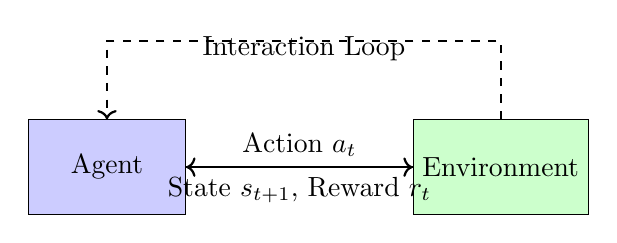
\begin{tikzpicture}[
    box/.style={rectangle, draw, minimum width=20mm, minimum height=12mm, align=center},
    agent/.style={fill=blue!20},
    env/.style={fill=green!20}
]
\node[box, agent] (agent) at (0,0) {Agent};
\node[box, env] (env) at (5,0) {Environment};

\draw[->, thick] (agent.east) -- (env.west) node[midway, above] {Action $a_t$};
\draw[->, thick] (env.west) -- (agent.east) node[midway, below] {State $s_{t+1}$, Reward $r_t$};

\draw[->, thick, dashed] (env.north) -- ++(0,1) -| (agent.north);
\node at (2.5, 1.5) {Interaction Loop};
\end{tikzpicture}
\caption{Agent-Environment interaction in RL}
\end{figure}

\begin{intuition}
Think of learning to play a video game:
\begin{itemize}
\item \textbf{State}: Current game screen
\item \textbf{Action}: Button presses (up, down, left, right, jump)
\item \textbf{Reward}: Points gained, lives lost
\item \textbf{Policy}: Strategy for playing (e.g., ``when enemy approaches, jump'')
\item \textbf{Goal}: Maximize total score (cumulative reward)
\end{itemize}

The agent explores different actions, observes rewards, and learns which actions lead to high scores.
\end{intuition}

\subsection{The Exploration-Exploitation Dilemma}

\begin{definition}[Exploration vs Exploitation]
\textbf{Exploitation}: Choose the best-known action (maximize immediate reward)

\textbf{Exploration}: Try new actions to discover potentially better options

\textbf{Dilemma}: How to balance?
\begin{itemize}
\item Pure exploitation: May miss better strategies
\item Pure exploration: Wastes time on known bad actions
\end{itemize}

\textbf{$\epsilon$-Greedy Strategy}:
\[
a_t = \begin{cases}
\argmax_a Q(s_t, a) & \text{with probability } 1-\epsilon \text{ (exploit)} \\
\text{random action} & \text{with probability } \epsilon \text{ (explore)}
\end{cases}
\]
Common: Start with high $\epsilon$ (e.g., 1.0), decay over time to 0.01.
\end{definition}

\subsection{Q-Learning}

\begin{definition}[Q-Learning]
Model-free algorithm to learn optimal Q-function (and thus optimal policy).

\textbf{Bellman Optimality Equation}:
\[
Q^*(s,a) = \E_{s' \sim P(\cdot|s,a)}\left[r(s,a) + \gamma \max_{a'} Q^*(s', a')\right]
\]
The optimal Q-value equals expected immediate reward plus discounted max future Q-value. In deterministic environments, this simplifies to $Q^*(s,a) = r + \gamma \max_{a'} Q^*(s', a')$.

\textbf{Q-Learning Update Rule}:
\[
Q(s_t, a_t) \leftarrow Q(s_t, a_t) + \alpha\left[r_t + \gamma \max_{a} Q(s_{t+1}, a) - Q(s_t, a_t)\right]
\]
where $\alpha$ is the learning rate.

\textbf{Intuition}: Adjust Q-value toward the observed return (TD error).
\end{definition}

\begin{algorithmbox}
\textbf{Q-Learning Algorithm}

\textbf{Initialize}: Q-table $Q(s,a) = 0$ for all states $s$ and actions $a$

\textbf{For} each episode:
\begin{enumerate}
\item Initialize state $s$
\item \textbf{While} not terminal:
\begin{itemize}
\item Choose action $a$ using $\epsilon$-greedy policy based on $Q(s, \cdot)$
\item Take action $a$, observe reward $r$ and next state $s'$
\item Update: 
\[
Q(s,a) \leftarrow Q(s,a) + \alpha\left[r + \gamma \max_{a'} Q(s',a') - Q(s,a)\right]
\]
\item $s \leftarrow s'$
\end{itemize}
\end{enumerate}

\textbf{Output}: Learned Q-table, optimal policy $\pi^*(s) = \argmax_a Q(s,a)$
\end{algorithmbox}

\begin{example}[GridWorld Navigation]
Agent in $4 \times 4$ grid, goal at top-right corner.

\textbf{States}: Grid positions
\textbf{Actions}: $\{\text{up, down, left, right}\}$
\textbf{Rewards}: $-1$ per step, $+10$ at goal, $-10$ for obstacles

Q-learning discovers shortest path by learning Q-values for each (state, action) pair.
\end{example}

\subsection{Deep Q-Networks (DQN)}

\begin{definition}[DQN]
Extend Q-learning to high-dimensional state spaces (e.g., images) using neural networks.

Instead of Q-table, use neural network $Q(s, a; \theta)$ parameterized by $\theta$.

\textbf{Key innovations}:

\textbf{1. Experience Replay}:
\begin{itemize}
\item Store transitions $(s_t, a_t, r_t, s_{t+1})$ in replay buffer
\item Sample random mini-batches for training
\item Breaks correlation between consecutive samples
\end{itemize}

\textbf{2. Target Network}:
\begin{itemize}
\item Use separate network $Q(s, a; \theta^-)$ for target computation
\item Update $\theta^-$ periodically (copy from $\theta$)
\item Stabilizes training (target doesn't move every update)
\end{itemize}

\textbf{Loss Function}:
\[
\Loss(\theta) = \E_{(s,a,r,s') \sim \text{Buffer}}\left[\left(r + \gamma \max_{a'} Q(s', a'; \theta^-) - Q(s, a; \theta)\right)^2\right]
\]
\end{definition}

\begin{keyidea}
\textbf{DQN Breakthroughs}:

\textbf{Success}: DQN (2013-2015) achieved human-level performance on Atari games using only pixel input.

\textbf{Why important}:
\begin{itemize}
\item First deep RL success on complex tasks
\item Showed RL can work with raw sensory input
\item Sparked modern deep RL research
\end{itemize}

\textbf{Extensions}:
\begin{itemize}
\item \textbf{Double DQN}: Addresses overestimation bias
\item \textbf{Dueling DQN}: Separate value and advantage streams
\item \textbf{Prioritized Experience Replay}: Sample important transitions more
\item \textbf{Rainbow}: Combines multiple improvements
\end{itemize}

\textbf{Limitations}:
\begin{itemize}
\item Sample inefficient (needs millions of frames)
\item Discrete actions only
\item Can be unstable
\end{itemize}
\end{keyidea}

\subsection{Policy Gradient Methods}

\begin{definition}[Policy Gradient]
Instead of learning Q-function, directly learn policy $\pi(a|s; \theta)$.

\textbf{Objective}: Maximize expected cumulative reward
\[
J(\theta) = \E_{\tau \sim \pi_\theta}\left[\sum_t r_t\right]
\]

\textbf{Policy Gradient Theorem}:
\[
\nabla_\theta J(\theta) = \E_{\tau \sim \pi_\theta}\left[\sum_t \nabla_\theta \log \pi_\theta(a_t|s_t) \cdot G_t\right]
\]
where $G_t = \sum_{k=t}^\infty \gamma^{k-t} r_k$ is return from time $t$.

\textbf{Intuition}: Increase probability of actions that led to high returns.
\end{definition}

\textbf{Modern Algorithms}:
\begin{itemize}
\item \textbf{REINFORCE}: Basic policy gradient
\item \textbf{Actor-Critic}: Combines policy gradient with value function
\item \textbf{A3C}: Asynchronous actor-critic
\item \textbf{PPO (Proximal Policy Optimization)}: State-of-the-art, stable
\item \textbf{SAC (Soft Actor-Critic)}: Maximum entropy RL
\end{itemize}

\subsection{Applications of RL}

\begin{itemize}
\item \textbf{Game Playing}: AlphaGo, OpenAI Five (Dota 2), AlphaStar (StarCraft)
\item \textbf{Robotics}: Manipulation, locomotion, drone control
\item \textbf{Autonomous Vehicles}: Path planning, decision making
\item \textbf{Recommendation Systems}: Sequential recommendations
\item \textbf{Resource Management}: Data center cooling, traffic light control
\item \textbf{Finance}: Trading, portfolio management
\item \textbf{Healthcare}: Treatment optimization, drug dosing
\end{itemize}

% =======================
\section{Representation Learning}
% =======================

\subsection{Introduction to Representation Learning}

\begin{definition}[Representation Learning]
Learning good representations (features) of data automatically, rather than hand-crafting them.

\textbf{Goal}: Discover abstractions that make it easier to extract useful information for downstream tasks.

\textbf{Good representations}:
\begin{itemize}
\item Capture relevant factors of variation
\item Disentangle underlying causes
\item Robust to noise
\item Transfer across tasks
\end{itemize}
\end{definition}

\subsection{Autoencoders}

\begin{definition}[Autoencoder]
Neural network trained to reconstruct its input through a bottleneck.

\textbf{Architecture}:
\begin{itemize}
\item \textbf{Encoder}: $\vect{z} = f_{\text{enc}}(\vect{x})$ (compress to latent code)
\item \textbf{Decoder}: $\hat{\vect{x}} = f_{\text{dec}}(\vect{z})$ (reconstruct)
\end{itemize}

\textbf{Training}: Minimize reconstruction error
\[
\Loss = \frac{1}{n}\sum_{i=1}^n \norm{\vect{x}_i - \hat{\vect{x}}_i}^2
\]

The bottleneck forces the network to learn compressed, meaningful representations.
\end{definition}

\begin{figure}[H]
\centering
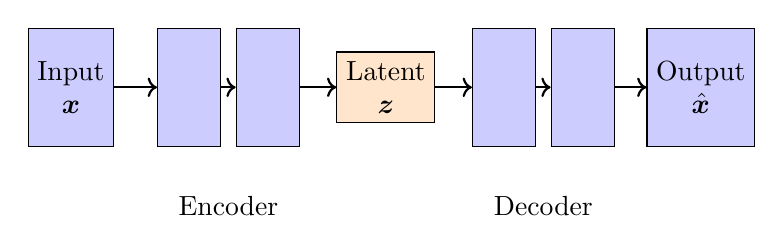
\begin{tikzpicture}[
    layer/.style={rectangle, draw, minimum width=8mm, minimum height=15mm, fill=blue!20},
    latent/.style={rectangle, draw, minimum width=8mm, minimum height=8mm, fill=orange!20}
]
% Input
\node[layer] (in) at (0,0) {Input\\$\vect{x}$};

% Encoder
\node[layer] (e1) at (1.5,0) {};
\node[layer] (e2) at (2.5,0) {};

% Latent
\node[latent] (z) at (4,0) {Latent\\$\vect{z}$};

% Decoder
\node[layer] (d1) at (5.5,0) {};
\node[layer] (d2) at (6.5,0) {};

% Output
\node[layer] (out) at (8,0) {Output\\$\hat{\vect{x}}$};

% Connections
\draw[->, thick] (in) -- (e1);
\draw[->, thick] (e1) -- (e2);
\draw[->, thick] (e2) -- (z);
\draw[->, thick] (z) -- (d1);
\draw[->, thick] (d1) -- (d2);
\draw[->, thick] (d2) -- (out);

% Labels
\node at (2, -1.5) {Encoder};
\node at (6, -1.5) {Decoder};
\end{tikzpicture}
\caption{Autoencoder architecture: compression and reconstruction}
\end{figure}

\subsubsection{Variants of Autoencoders}

\begin{definition}[Autoencoder Variants]

\textbf{1. Denoising Autoencoder (DAE)}:
\begin{itemize}
\item Input: Corrupted version $\tilde{\vect{x}}$ (add noise)
\item Target: Original clean $\vect{x}$
\item Forces learning robust features
\end{itemize}

\textbf{2. Sparse Autoencoder}:
\begin{itemize}
\item Add sparsity penalty: $\Loss = \text{reconstruction} + \lambda \sum_j |z_j|$
\item Encourages few active latent units
\end{itemize}

\textbf{3. Variational Autoencoder (VAE)}:
\begin{itemize}
\item Learns probability distribution $p(\vect{z}|\vect{x})$
\item Encoder outputs $\mu$ and $\sigma$ of Gaussian
\item Can generate new samples by sampling from $p(\vect{z})$
\item Loss: $\Loss = \text{reconstruction} + \text{KL}(q(\vect{z}|\vect{x}) \| p(\vect{z}))$
\end{itemize}

\textbf{4. Contractive Autoencoder}:
\begin{itemize}
\item Penalizes sensitivity of encoding to input perturbations
\item More robust representations
\end{itemize}
\end{definition}

\begin{keyidea}
\textbf{Applications of Autoencoders}:
\begin{itemize}
\item \textbf{Dimensionality reduction}: Alternative to PCA (non-linear)
\item \textbf{Anomaly detection}: High reconstruction error $\to$ anomaly
\item \textbf{Denoising}: Remove noise from images, audio
\item \textbf{Data generation}: VAEs generate new samples
\item \textbf{Feature learning}: Use latent codes as features for downstream tasks
\item \textbf{Pretraining}: Initialize networks for supervised learning
\end{itemize}
\end{keyidea}

\subsection{Word Embeddings}

\subsubsection{Motivation}

\begin{definition}[Word Representation Problem]
How to represent words for machine learning?

\textbf{One-hot encoding}:
\[
\text{``cat''} = [0, 0, 1, 0, \ldots, 0], \quad \text{``dog''} = [0, 0, 0, 1, \ldots, 0]
\]

\textbf{Problems}:
\begin{itemize}
\item High-dimensional ($|V|$ for vocabulary size)
\item Sparse (only one 1)
\item No semantic similarity (all words equally distant)
\end{itemize}

\textbf{Solution}: Dense, low-dimensional embeddings that capture semantics.
\end{definition}

\subsubsection{Word2Vec}

\begin{definition}[Word2Vec]
Learn word embeddings by predicting context words.

\textbf{Two architectures}:

\textbf{1. CBOW (Continuous Bag of Words)}:
\begin{itemize}
\item Input: Context words
\item Output: Target (center) word
\item Predict word from its context
\end{itemize}

\textbf{2. Skip-gram}:
\begin{itemize}
\item Input: Target word
\item Output: Context words
\item Predict context from word
\end{itemize}

\textbf{Training objective} (Skip-gram):
\[
\max \frac{1}{T}\sum_{t=1}^T \sum_{-c \leq j \leq c, j \neq 0} \log P(w_{t+j} | w_t)
\]
where $c$ is context window size.

\textbf{Probability}:
\[
P(w_O | w_I) = \frac{\exp(\vect{v}_{w_O}^\top \vect{v}_{w_I})}{\sum_{w \in V} \exp(\vect{v}_w^\top \vect{v}_{w_I})}
\]
\end{definition}

\begin{keyidea}
\textbf{Word2Vec Properties}:

\textbf{Semantic similarity}:
\begin{itemize}
\item Similar words have similar embeddings
\item $\text{similarity}(\text{``cat''}, \text{``dog''}) > \text{similarity}(\text{``cat''}, \text{``car''})$
\end{itemize}

\textbf{Analogies}:
\[
\vect{v}_{\text{king}} - \vect{v}_{\text{man}} + \vect{v}_{\text{woman}} \approx \vect{v}_{\text{queen}}
\]
Vector arithmetic captures relationships!

\textbf{Composition}:
\begin{itemize}
\item ``New York'' = embedding of ``New'' + embedding of ``York''
\end{itemize}

\textbf{Training efficiency}:
\begin{itemize}
\item Negative sampling: Instead of full softmax over $|V|$, sample few negative examples
\item Hierarchical softmax: Use tree structure for faster computation
\end{itemize}
\end{keyidea}

\subsubsection{GloVe}

\begin{definition}[GloVe (Global Vectors)]
Learn embeddings by factorizing word co-occurrence matrix.

\textbf{Objective}:
\[
J = \sum_{i,j=1}^{|V|} f(X_{ij})(\vect{w}_i^\top \tilde{\vect{w}}_j + b_i + \tilde{b}_j - \log X_{ij})^2
\]
where:
\begin{itemize}
\item $X_{ij}$: Number of times word $j$ appears in context of word $i$
\item $f(X_{ij})$: Weighting function (down-weight rare co-occurrences)
\end{itemize}

\textbf{Advantage}: Uses global corpus statistics (Word2Vec uses local context).
\end{definition}

\subsection{Contrastive Learning}

\begin{definition}[Contrastive Learning]
Learn representations by contrasting similar and dissimilar examples.

\textbf{Core idea}: Pull similar examples together, push dissimilar ones apart in embedding space.

\textbf{SimCLR (Simple Framework for Contrastive Learning)}:
\begin{enumerate}
\item \textbf{Data augmentation}: Create two views of each image (crop, color jitter, etc.)
\item \textbf{Encode}: Pass through neural network $f(\cdot)$ to get embeddings
\item \textbf{Project}: Apply projection head $g(\cdot)$ to get $\vect{z}$
\item \textbf{Contrastive loss}:
\[
\ell_{i,j} = -\log \frac{\exp(\text{sim}(\vect{z}_i, \vect{z}_j)/\tau)}{\sum_{k=1}^{2N} \mathbbm{1}_{k \neq i} \exp(\text{sim}(\vect{z}_i, \vect{z}_k)/\tau)}
\]
where $\text{sim}(\vect{u}, \vect{v}) = \vect{u}^\top\vect{v} / (\norm{\vect{u}}\norm{\vect{v}})$ (cosine similarity).
\end{enumerate}
\end{definition}

\begin{keyidea}
\textbf{Why Contrastive Learning is Powerful}:

\textbf{Self-supervised}: No labels needed! Use data augmentation to create positive pairs.

\textbf{State-of-the-art results}:
\begin{itemize}
\item SimCLR: Competitive with supervised learning on ImageNet
\item MoCo (Momentum Contrast): Efficient contrastive learning
\item CLIP: Contrastive learning for image-text pairs (foundation of DALL-E)
\end{itemize}

\textbf{Applications}:
\begin{itemize}
\item Image classification (pretrain on unlabeled data)
\item Few-shot learning (good representations with few labels)
\item Transfer learning (transfer to downstream tasks)
\item Multi-modal learning (vision + language)
\end{itemize}

\textbf{Recent methods}:
\begin{itemize}
\item BYOL (Bootstrap Your Own Latent): No negative pairs needed
\item SimSiam: Even simpler, still effective
\item SwAV: Clustering-based contrastive learning
\end{itemize}
\end{keyidea}

% =======================
\section{Ethics and Fairness in Machine Learning}
% =======================

\subsection{Bias and Discrimination}

\begin{definition}[Types of Bias in ML]

\textbf{1. Data Bias}:
\begin{itemize}
\item \textbf{Historical bias}: Data reflects past discrimination
\item \textbf{Sampling bias}: Training data not representative of population
\item \textbf{Measurement bias}: Features measured differently for different groups
\end{itemize}

\textbf{2. Algorithmic Bias}:
\begin{itemize}
\item Model amplifies existing biases
\item Optimization objective doesn't account for fairness
\end{itemize}

\textbf{3. Interaction Bias}:
\begin{itemize}
\item Feedback loops: Biased predictions reinforce themselves
\item Example: Predictive policing $\to$ more arrests in certain areas $\to$ model predicts more crime there
\end{itemize}
\end{definition}

\begin{example}[Real-World Bias Cases]

\textbf{1. COMPAS (Recidivism Prediction)}:
\begin{itemize}
\item Predicted re-arrest risk for defendants
\item ProPublica investigation: Biased against African Americans
\item Higher false positive rate for Black defendants
\end{itemize}

\textbf{2. Hiring Algorithms}:
\begin{itemize}
\item Amazon scrapped ML hiring tool (2018)
\item Trained on historical data (mostly male applicants)
\item Penalized resumes with ``women's'' (e.g., ``women's chess club'')
\end{itemize}

\textbf{3. Facial Recognition}:
\begin{itemize}
\item Lower accuracy for women and people of color
\item Training data predominantly white males
\item Real consequences: wrongful arrests
\end{itemize}

\textbf{4. Credit Scoring}:
\begin{itemize}
\item ML models for loan approval
\item May discriminate based on proxy variables (zip code $\to$ race)
\end{itemize}
\end{example}

\subsection{Fairness Definitions}

\begin{definition}[Fairness Metrics]

\textbf{1. Demographic Parity (Statistical Parity)}:
\[
P(\hat{Y} = 1 | A = 0) = P(\hat{Y} = 1 | A = 1)
\]
Equal positive prediction rates across groups $A$ (e.g., race, gender).

\textbf{2. Equalized Odds}:
\[
P(\hat{Y} = 1 | Y = y, A = 0) = P(\hat{Y} = 1 | Y = y, A = 1) \quad \text{for } y \in \{0, 1\}
\]
Equal TPR and FPR across groups.

\textbf{3. Equal Opportunity}:
\[
P(\hat{Y} = 1 | Y = 1, A = 0) = P(\hat{Y} = 1 | Y = 1, A = 1)
\]
Equal TPR (recall) across groups. Subset of equalized odds.

\textbf{4. Predictive Parity}:
\[
P(Y = 1 | \hat{Y} = 1, A = 0) = P(Y = 1 | \hat{Y} = 1, A = 1)
\]
Equal precision across groups.

\textbf{5. Individual Fairness}:
Similar individuals should receive similar predictions (harder to formalize).
\end{definition}

\begin{keyidea}
\textbf{Fairness Trade-offs}:

\textbf{Impossibility results}: Cannot satisfy all fairness definitions simultaneously (except in trivial cases).

\textbf{Accuracy vs Fairness}: Often a trade-off
\begin{itemize}
\item Unconstrained model: Highest accuracy, may be unfair
\item Fair model: Lower accuracy, satisfies fairness constraints
\end{itemize}

\textbf{Which fairness metric to use?}
\begin{itemize}
\item Depends on context and stakeholders
\item Medical diagnosis: Equal opportunity (equal TPR)
\item Advertising: Demographic parity
\item Criminal justice: Combination of metrics
\end{itemize}

\textbf{Mitigation strategies}:
\begin{itemize}
\item \textbf{Pre-processing}: Transform data to remove bias
\item \textbf{In-processing}: Add fairness constraints to training
\item \textbf{Post-processing}: Adjust predictions to satisfy fairness
\end{itemize}
\end{keyidea}

\subsection{Explainable AI (XAI)}

\begin{definition}[Explainability]
The ability to explain or present ML predictions in understandable terms to humans.

\textbf{Why important?}:
\begin{itemize}
\item Trust: Users need to trust model decisions
\item Debugging: Understand why model fails
\item Regulation: GDPR ``right to explanation''
\item Fairness: Detect and fix bias
\item Safety: Critical applications (healthcare, autonomous vehicles)
\end{itemize}
\end{definition}

\subsubsection{LIME (Local Interpretable Model-agnostic Explanations)}

\begin{definition}[LIME]
Explain individual predictions by approximating the model locally with an interpretable model.

\textbf{Algorithm}:
\begin{enumerate}
\item Select instance $\vect{x}$ to explain
\item Perturb $\vect{x}$ to create neighborhood samples
\item Get predictions from black-box model on perturbed samples
\item Fit simple interpretable model (e.g., linear regression) weighted by proximity to $\vect{x}$
\item Explain prediction using interpretable model's coefficients
\end{enumerate}

\textbf{Intuition}: Fit a simple model locally around the prediction to understand what features matter.
\end{definition}

\begin{example}[LIME for Image Classification]
Model predicts ``husky'' for an image.

LIME highlights image regions:
\begin{itemize}
\item Green regions: Support prediction (dog's face, fur)
\item Red regions: Against prediction (background)
\end{itemize}

Reveals: Model uses dog features (good) or background snow (bad---spurious correlation)?
\end{example}

\subsubsection{SHAP (SHapley Additive exPlanations)}

\begin{definition}[SHAP]
Uses Shapley values from cooperative game theory to assign each feature an importance value for a prediction.

\textbf{Shapley value}: Fair distribution of ``payout'' (prediction) among ``players'' (features).

\textbf{Properties}:
\begin{itemize}
\item \textbf{Local accuracy}: Explanation matches prediction
\item \textbf{Consistency}: If feature contributes more, importance increases
\item \textbf{Missingness}: Feature not used $\to$ zero importance
\end{itemize}

\textbf{Computation}:
\[
\phi_i = \sum_{S \subseteq F \setminus \{i\}} \frac{|S|!(|F|-|S|-1)!}{|F|!}[f(S \cup \{i\}) - f(S)]
\]
Average marginal contribution of feature $i$ across all feature subsets.

\textbf{Advantages over LIME}:
\begin{itemize}
\item Theoretical foundation (game theory)
\item Consistent across models
\item Can aggregate for global explanations
\end{itemize}
\end{definition}

\begin{implementationbox}
\textbf{Using SHAP in Python}:

\begin{lstlisting}[language=Python]
import shap

# Train model
model = RandomForestClassifier()
model.fit(X_train, y_train)

# Create explainer
explainer = shap.TreeExplainer(model)

# Compute SHAP values
shap_values = explainer.shap_values(X_test)

# Visualize
shap.summary_plot(shap_values, X_test)  # Global
shap.force_plot(explainer.expected_value, 
                shap_values[0], X_test.iloc[0])  # Local
\end{lstlisting}
\end{implementationbox}

\subsubsection{Other Interpretability Methods}

\begin{itemize}
\item \textbf{Attention Mechanisms}: In Transformers, attention weights show which input tokens are important
\item \textbf{Saliency Maps}: Gradient-based methods for images (highlight important pixels)
\item \textbf{Partial Dependence Plots (PDP)}: Show relationship between feature and prediction
\item \textbf{Counterfactual Explanations}: ``What would need to change for different prediction?''
\item \textbf{Anchors}: Find sufficient conditions for prediction (``If age > 50 AND income > 100K, then approve'')
\end{itemize}

\subsection{Responsible AI Practices}

\begin{tcolorbox}[colback=red!5!white,colframe=red!75!black,title=Guidelines for Ethical ML]
\begin{enumerate}
\item \textbf{Diverse Teams}: Include diverse perspectives in development

\item \textbf{Data Auditing}: Check training data for bias, representativeness

\item \textbf{Fairness Testing}: Evaluate model across demographic groups

\item \textbf{Transparency}: Document data sources, model architecture, limitations

\item \textbf{Human Oversight}: Keep humans in the loop for critical decisions

\item \textbf{Regular Audits}: Monitor model performance and fairness in production

\item \textbf{Right to Appeal}: Allow users to contest automated decisions

\item \textbf{Privacy}: Protect user data, use privacy-preserving techniques (differential privacy, federated learning)

\item \textbf{Impact Assessment}: Consider societal impact before deployment

\item \textbf{Continuous Learning}: Stay updated on fairness research and regulations
\end{enumerate}
\end{tcolorbox}

% =======================
\section{Modern Trends}
% =======================

\subsection{Transfer Learning and Fine-Tuning}

\begin{definition}[Transfer Learning]
Use knowledge learned from one task (source) to improve learning on a different but related task (target).

\textbf{Why transfer?}
\begin{itemize}
\item Limited labeled data for target task
\item Training from scratch is expensive
\item Pretrained models capture general features
\end{itemize}

\textbf{Typical workflow}:
\begin{enumerate}
\item \textbf{Pretrain}: Train model on large dataset (e.g., ImageNet)
\item \textbf{Transfer}: Use pretrained weights as initialization
\item \textbf{Fine-tune}: Train on target task with small learning rate
\end{enumerate}
\end{definition}

\begin{keyidea}
\textbf{Transfer Learning Strategies}:

\textbf{1. Feature Extraction} (Frozen Pretrained Model):
\begin{itemize}
\item Freeze all pretrained layers
\item Add new layers on top
\item Train only new layers
\item Fast, works when target data is small and similar to source
\end{itemize}

\textbf{2. Fine-Tuning All Layers}:
\begin{itemize}
\item Unfreeze all layers
\item Train entire network with small learning rate
\item Best performance, needs more target data
\end{itemize}

\textbf{3. Fine-Tuning Top Layers Only}:
\begin{itemize}
\item Freeze early layers (general features)
\item Unfreeze later layers (task-specific features)
\item Balance between feature extraction and full fine-tuning
\end{itemize}

\textbf{Success stories}:
\begin{itemize}
\item \textbf{Computer Vision}: ResNet, EfficientNet pretrained on ImageNet
\item \textbf{NLP}: BERT, GPT pretrained on massive text corpora
\item \textbf{Speech}: Wav2Vec2 pretrained on unlabeled audio
\end{itemize}
\end{keyidea}

\subsection{Foundation Models}

\begin{definition}[Foundation Models]
Large-scale models trained on broad data that can be adapted to a wide range of downstream tasks.

\textbf{Characteristics}:
\begin{itemize}
\item Trained on massive diverse datasets (web-scale)
\item Billions of parameters
\item Emergent capabilities (not explicitly trained for)
\item General-purpose (adapt to many tasks)
\end{itemize}

\textbf{Paradigm shift}: 
\[
\text{Traditional: Task-specific data} \to \text{Task-specific model}
\]
\[
\text{Foundation: General data} \to \text{Foundation model} \to \text{Many tasks}
\]
\end{definition}

\subsubsection{BERT (Bidirectional Encoder Representations from Transformers)}

\begin{definition}[BERT]
Pretrained Transformer encoder (2018, Google).

\textbf{Pretraining tasks}:
\begin{itemize}
\item \textbf{Masked Language Modeling (MLM)}: Mask 15\% of tokens, predict them
\[
\text{Input: } \text{The [MASK] is on the table}
\]
\[
\text{Predict: } \text{cat}
\]
\item \textbf{Next Sentence Prediction (NSP)}: Predict if sentence B follows sentence A
\end{itemize}

\textbf{Impact}:
\begin{itemize}
\item State-of-the-art on many NLP tasks
\item Spawned many variants (RoBERTa, ALBERT, DistilBERT)
\item Showed power of bidirectional context
\end{itemize}
\end{definition}

\subsubsection{GPT (Generative Pre-trained Transformer)}

\begin{definition}[GPT Family]
Autoregressive Transformer decoders (OpenAI).

\textbf{GPT-1} (2018): 117M parameters
\textbf{GPT-2} (2019): 1.5B parameters
\textbf{GPT-3} (2020): 175B parameters
\textbf{GPT-4} (2023): Estimated $>$1T parameters (multimodal)

\textbf{Training}: Predict next token given previous tokens
\[
P(w_t | w_1, \ldots, w_{t-1})
\]

\textbf{Key insight}: Scale $+$ next token prediction $=$ emergent abilities
\begin{itemize}
\item Few-shot learning: Learn from few examples in prompt
\item In-context learning: Adapt to task from prompt alone
\item Chain-of-thought reasoning: Generate step-by-step solutions
\end{itemize}
\end{definition}

\begin{keyidea}
\textbf{GPT-3 Capabilities}:

\textbf{Zero-shot}: No examples, just task description
\begin{verbatim}
Translate to French: Hello, how are you?
Output: Bonjour, comment allez-vous?
\end{verbatim}

\textbf{Few-shot}: Provide examples in prompt
\begin{verbatim}
Q: What is 2+2? A: 4
Q: What is 5+3? A: 8
Q: What is 7+9? A: 16
\end{verbatim}

\textbf{Emergent abilities} (not seen in smaller models):
\begin{itemize}
\item Arithmetic
\item Code generation
\item Common sense reasoning
\item Instruction following
\end{itemize}

\textbf{Limitations}:
\begin{itemize}
\item Hallucinations (generates plausible but false information)
\item Bias from training data
\item No grounding in real world
\item Expensive to run
\end{itemize}
\end{keyidea}

\subsection{Federated Learning}

\begin{definition}[Federated Learning]
Train models across decentralized devices without sharing raw data.

\textbf{Workflow}:
\begin{enumerate}
\item Server sends global model to clients
\item Each client trains on local data
\item Clients send model updates (not data) to server
\item Server aggregates updates into global model
\item Repeat
\end{enumerate}

\textbf{Aggregation} (FedAvg):
\[
\vect{w}_{t+1} = \sum_{k=1}^K \frac{n_k}{n} \vect{w}_k^{(t)}
\]
Weighted average of client models by data size.
\end{definition}

\begin{keyidea}
\textbf{Benefits of Federated Learning}:
\begin{itemize}
\item \textbf{Privacy}: Data never leaves device
\item \textbf{Reduced latency}: On-device inference
\item \textbf{Regulatory compliance}: GDPR, HIPAA
\item \textbf{Bandwidth efficiency}: Share models, not data
\end{itemize}

\textbf{Challenges}:
\begin{itemize}
\item \textbf{Non-IID data}: Each client has different distribution
\item \textbf{Communication cost}: Many rounds needed
\item \textbf{Heterogeneous devices}: Different compute power
\item \textbf{Privacy attacks}: Model updates can leak information
\end{itemize}

\textbf{Applications}:
\begin{itemize}
\item Mobile keyboards (Gboard)
\item Healthcare (multiple hospitals, can't share patient data)
\item Finance (banks collaborate without sharing data)
\item IoT devices
\end{itemize}

\textbf{Enhanced privacy}:
\begin{itemize}
\item Differential privacy: Add noise to updates
\item Secure aggregation: Encrypted updates
\item Homomorphic encryption: Compute on encrypted data
\end{itemize}
\end{keyidea}

\subsection{AutoML (Automated Machine Learning)}

\begin{definition}[AutoML]
Automate the end-to-end process of applying ML to real-world problems.

\textbf{Components}:
\begin{itemize}
\item Data preprocessing
\item Feature engineering
\item Model selection
\item Hyperparameter optimization
\item Architecture search (for neural networks)
\item Ensemble construction
\end{itemize}
\end{definition}

\subsubsection{Neural Architecture Search (NAS)}

\begin{definition}[NAS]
Automatically design neural network architectures.

\textbf{Search space}: Define possible architectures (layers, connections, operations)

\textbf{Search strategy}:
\begin{itemize}
\item Random search
\item Reinforcement learning
\item Evolutionary algorithms
\item Gradient-based (DARTS)
\end{itemize}

\textbf{Performance estimation}:
\begin{itemize}
\item Train from scratch (expensive)
\item Early stopping
\item Weight sharing (ENAS)
\item Performance prediction
\end{itemize}

\textbf{Success}: NAS-discovered architectures (EfficientNet, AmoebaNet) outperform hand-designed ones.
\end{definition}

\subsubsection{AutoML Tools}

\begin{itemize}
\item \textbf{Auto-sklearn}: Automated scikit-learn pipeline
\item \textbf{TPOT}: Genetic programming for pipeline optimization
\item \textbf{H2O AutoML}: Automated model selection and ensembling
\item \textbf{Google Cloud AutoML}: Managed AutoML service
\item \textbf{AutoKeras}: NAS for Keras
\item \textbf{PyCaret}: Low-code ML library
\end{itemize}

\begin{keyidea}
\textbf{AutoML: Democratization or Threat?}

\textbf{Pros}:
\begin{itemize}
\item Lowers barrier to entry (non-experts can use ML)
\item Frees experts to focus on problem formulation
\item Often finds better models than manual search
\item Reproducible workflows
\end{itemize}

\textbf{Cons}:
\begin{itemize}
\item Can be slow (lots of trials)
\item Black box (hard to understand choices)
\item May not consider domain constraints
\item Expensive (compute cost)
\end{itemize}

\textbf{Reality}: AutoML is a tool, not a replacement. ML expertise still needed for:
\begin{itemize}
\item Problem formulation
\item Data quality assessment
\item Interpreting results
\item Debugging failures
\item Ethical considerations
\end{itemize}
\end{keyidea}

\subsection{Future Directions}

\begin{keyidea}
\textbf{Emerging Trends and Open Problems}:

\textbf{1. Multimodal Learning}:
\begin{itemize}
\item Models that understand multiple modalities (text, image, audio, video)
\item CLIP, DALL-E, Flamingo, GPT-4
\end{itemize}

\textbf{2. Continual Learning}:
\begin{itemize}
\item Learn new tasks without forgetting old ones
\item Overcome catastrophic forgetting
\end{itemize}

\textbf{3. Few-Shot and Zero-Shot Learning}:
\begin{itemize}
\item Learn from very few examples
\item Generalize to unseen classes
\end{itemize}

\textbf{4. Causal Machine Learning}:
\begin{itemize}
\item Go beyond correlation to causation
\item Robust to distribution shift
\item Counterfactual reasoning
\end{itemize}

\textbf{5. Energy-Efficient ML}:
\begin{itemize}
\item Reduce environmental impact (training GPT-3: tons of CO2)
\item Model compression, pruning, quantization
\item Efficient architectures
\end{itemize}

\textbf{6. Trustworthy AI}:
\begin{itemize}
\item Robustness to adversarial attacks
\item Uncertainty quantification
\item Certified defenses
\end{itemize}

\textbf{7. Human-AI Collaboration}:
\begin{itemize}
\item AI as assistant, not replacement
\item Interactive ML
\item Human-in-the-loop systems
\end{itemize}

\textbf{8. Quantum Machine Learning}:
\begin{itemize}
\item Leverage quantum computers for ML
\item Quantum neural networks
\item Early stage, potential for exponential speedups
\end{itemize}
\end{keyidea}

\subsection{Conclusion}

\begin{tcolorbox}[colback=green!5!white,colframe=green!75!black,title=Final Thoughts]
Machine Learning is a rapidly evolving field with profound impact on society. As practitioners, we must:

\begin{enumerate}
\item \textbf{Master fundamentals}: Strong foundation enables understanding new methods

\item \textbf{Stay curious}: New papers, techniques, applications emerge daily

\item \textbf{Think critically}: Not every problem needs ML; not every solution is ethical

\item \textbf{Embrace uncertainty}: Models are tools, not truth

\item \textbf{Prioritize ethics}: Consider impact on individuals and society

\item \textbf{Collaborate}: ML is interdisciplinary---work with domain experts

\item \textbf{Keep learning}: The field evolves faster than any textbook
\end{enumerate}

The journey from mathematical foundations to modern foundation models is remarkable. Yet the most exciting developments are still ahead. Whether through scientific breakthroughs, ethical frameworks, or novel applications, the future of ML will be shaped by thoughtful practitioners who combine technical skill with wisdom.

\textbf{Your role}: Build systems that are not just intelligent, but beneficial.
\end{tcolorbox}

\begin{exercise}
\begin{enumerate}
\item Design a Q-learning agent for a simple grid world. Define states, actions, rewards, and write the Q-update rule.

\item Explain why experience replay and target networks are crucial for DQN stability. What problems do they solve?

\item Compare PCA (from Part 5) and autoencoders for dimensionality reduction. When would you prefer autoencoders?

\item Given Word2Vec embeddings, explain why $\vect{v}_{\text{king}} - \vect{v}_{\text{man}} + \vect{v}_{\text{woman}} \approx \vect{v}_{\text{queen}}$ works. What does this reveal about the embedding space?

\item A facial recognition system has 99\% accuracy but 5\% false positive rate for one demographic group vs 1\% for another. Which fairness definition is violated? Propose a mitigation strategy.

\item You have 100 labeled examples and 10,000 unlabeled examples for image classification. Design a strategy using transfer learning and/or contrastive learning.

\item Compare fine-tuning BERT for sentiment analysis vs training a CNN from scratch. What are the trade-offs?

\item Design a federated learning system for predicting disease from hospital data. Address: communication efficiency, privacy, and non-IID data distributions.
\end{enumerate}
\end{exercise}

\vspace{1cm}

\begin{center}
\Large\textbf{End of Machine Learning Notes}

\vspace{0.5cm}

\textit{``The best way to predict the future is to invent it.'' --- Alan Kay}
\end{center}

\end{document}